\documentclass[a4paper,11pt]{article}
\usepackage{amsmath,amssymb,graphicx,hyperref}
\usepackage[margin=1in]{geometry}
\usepackage{booktabs}
\usepackage{multirow}
\graphicspath{{figures/}}

\title{Early Dark Energy and the Geometric Ceiling: Constraints from Planck, ACT DR6, and DESI Y1}
\author{Steven Ridder\\
\textit{Independent Researcher, United States}\\
\texttt{sridder@post.harvard.edu}}
\date{\today}

\begin{document}

\maketitle

\begin{abstract}
The standard cosmological model $\Lambda$CDM continues to fit most data sets extremely well, but it favors a low expansion rate $H_0 \simeq 68$~km~s$^{-1}$~Mpc$^{-1}$ that is in tension with several modern late-time measurements. Recent JWST, TRGB, and strong-lens analyses instead cluster around $H_0 \simeq 69$--$71$~km~s$^{-1}$~Mpc$^{-1}$, while weak-lensing surveys prefer $S_8 \simeq 0.76$--$0.80$. We introduce a simple scalar field extension, ``Geometric EDE,'' that modifies the pre-recombination expansion history and treats these anomalies as a single geometric problem. The field briefly contributes a few percent of the total energy density near redshift $z \sim 3000$, slightly shrinks the sound horizon, raises the CMB-inferred Hubble constant toward $H_0 \simeq 70$~km~s$^{-1}$~Mpc$^{-1}$, and modestly suppresses $S_8$ while preserving the acoustic peak structure of the CMB.

In pre-DESI combinations of Planck, BAO, and local $H_0$ data, this model reduces the $H_0$ tension from about $4.3\sigma$ to $2.3\sigma$ and the $S_8$ tension from about $2.7\sigma$ to $1.1\sigma$, with an overall improvement $\Delta\chi^2 \simeq -4.5$ relative to $\Lambda$CDM for two additional parameters. Once DESI Y1 BAO are included, fixed-$H_0$ profile likelihoods reveal a \emph{geometric ceiling}: $\Delta\chi^2$ rises from $\simeq +2$ at $H_0 = 69$ to $\simeq +15$ at $H_0 = 70$ and $\gtrsim 90$ by $H_0 = 72$, so early-time physics alone cannot reach the original SH0ES target near $73$~km~s$^{-1}$~Mpc$^{-1}$. We trace this ceiling to a \emph{correlation flip} in the Planck+DESI posterior: DESI reverses the sign of the correlation between EDE amplitude and reionization optical depth, which closes a degeneracy where low-$\ell$ polarization could previously compensate the damping-tail cost. Stress-test runs show that forcing $\Lambda$CDM into the same $H_0 \simeq 70$ convergence window would incur a penalty $\Delta\chi^2 \gtrsim 30$--$40$ while worsening $S_8$.

The same physics predicts a characteristic ``soft shoulder'' in the CMB damping tail at the one-percent level. We construct a fixed template for this ripple pattern and fit its amplitude to ACT DR6 TT+EE data at fixed background cosmology, finding a $6.4\sigma$ preference for a nonzero shoulder aligned with the Geometric EDE template. Taken together, the geometric ceiling, the $H_0$--$S_8$ convergence window, and the soft-shoulder detection make early-time geometry a concrete and falsifiable alternative to purely late-time or systematic explanations of the current anomalies and provide a sharp target for upcoming CMB-S4 observations.
\end{abstract}

% =============================================================================
% SECTION I: INTRODUCTION
% =============================================================================

\section{Introduction}

\subsection{Current Observational Tensions}

The standard $\Lambda$CDM cosmological model provides an excellent fit to Planck 2018 CMB data~\cite{Planck2018,Planck2018_params}, yielding $H_0 = 67.4 \pm 0.5$~km~s$^{-1}$~Mpc$^{-1}$ and a clustering amplitude $S_8 \equiv \sigma_8 \sqrt{\Omega_m/0.3} \simeq 0.83$. However, this CMB-inferred expansion rate is in tension with several late-time measurements~\cite{Kamionkowski_Riess,DiValentino_review}.

The SH0ES Cepheid-calibrated distance ladder reports $H_0 = 73.04 \pm 1.04$~km~s$^{-1}$~Mpc$^{-1}$~\cite{SH0ES}, differing from the Planck $\Lambda$CDM value at approximately $5\sigma$. This discrepancy, known as the Hubble tension, has motivated numerous extensions to the standard model~\cite{Knox_Millea}. More recently, JWST calibrations of the Tip of the Red Giant Branch (TRGB) yield $H_0 = 70.4 \pm 1.2$~km~s$^{-1}$~Mpc$^{-1}$~\cite{Freedman2024}, an intermediate value that suggests the discrepancy may be smaller than earlier estimates indicated.

Independently, cosmic shear measurements from KiDS~\cite{KiDS1000}, DES~\cite{DES_Y3}, and HSC~\cite{HSC_Y3} consistently prefer lower values of $S_8$ than the Planck $\Lambda$CDM prediction~\cite{DiValentino_S8}. The DES Year~3 analysis finds $S_8 = 0.776 \pm 0.017$, approximately $2\sigma$ below the Planck value. This clustering tension is less significant than the Hubble discrepancy but is persistent across surveys.

These tensions present a challenge for model building. Extensions that raise $H_0$ by modifying late-time dynamics often worsen the fit to BAO and supernovae or increase $S_8$~\cite{Mortsell_Dhawan}. Models that reduce $S_8$ through modified gravity can conflict with CMB constraints and fifth-force bounds. Most proposed solutions ameliorate one tension at the cost of exacerbating another~\cite{Verde_H0}. In this work, we investigate whether a controlled modification of the pre-recombination expansion history can simultaneously address both the $H_0$ and $S_8$ discrepancies.

\begin{figure}[ht]
\centering
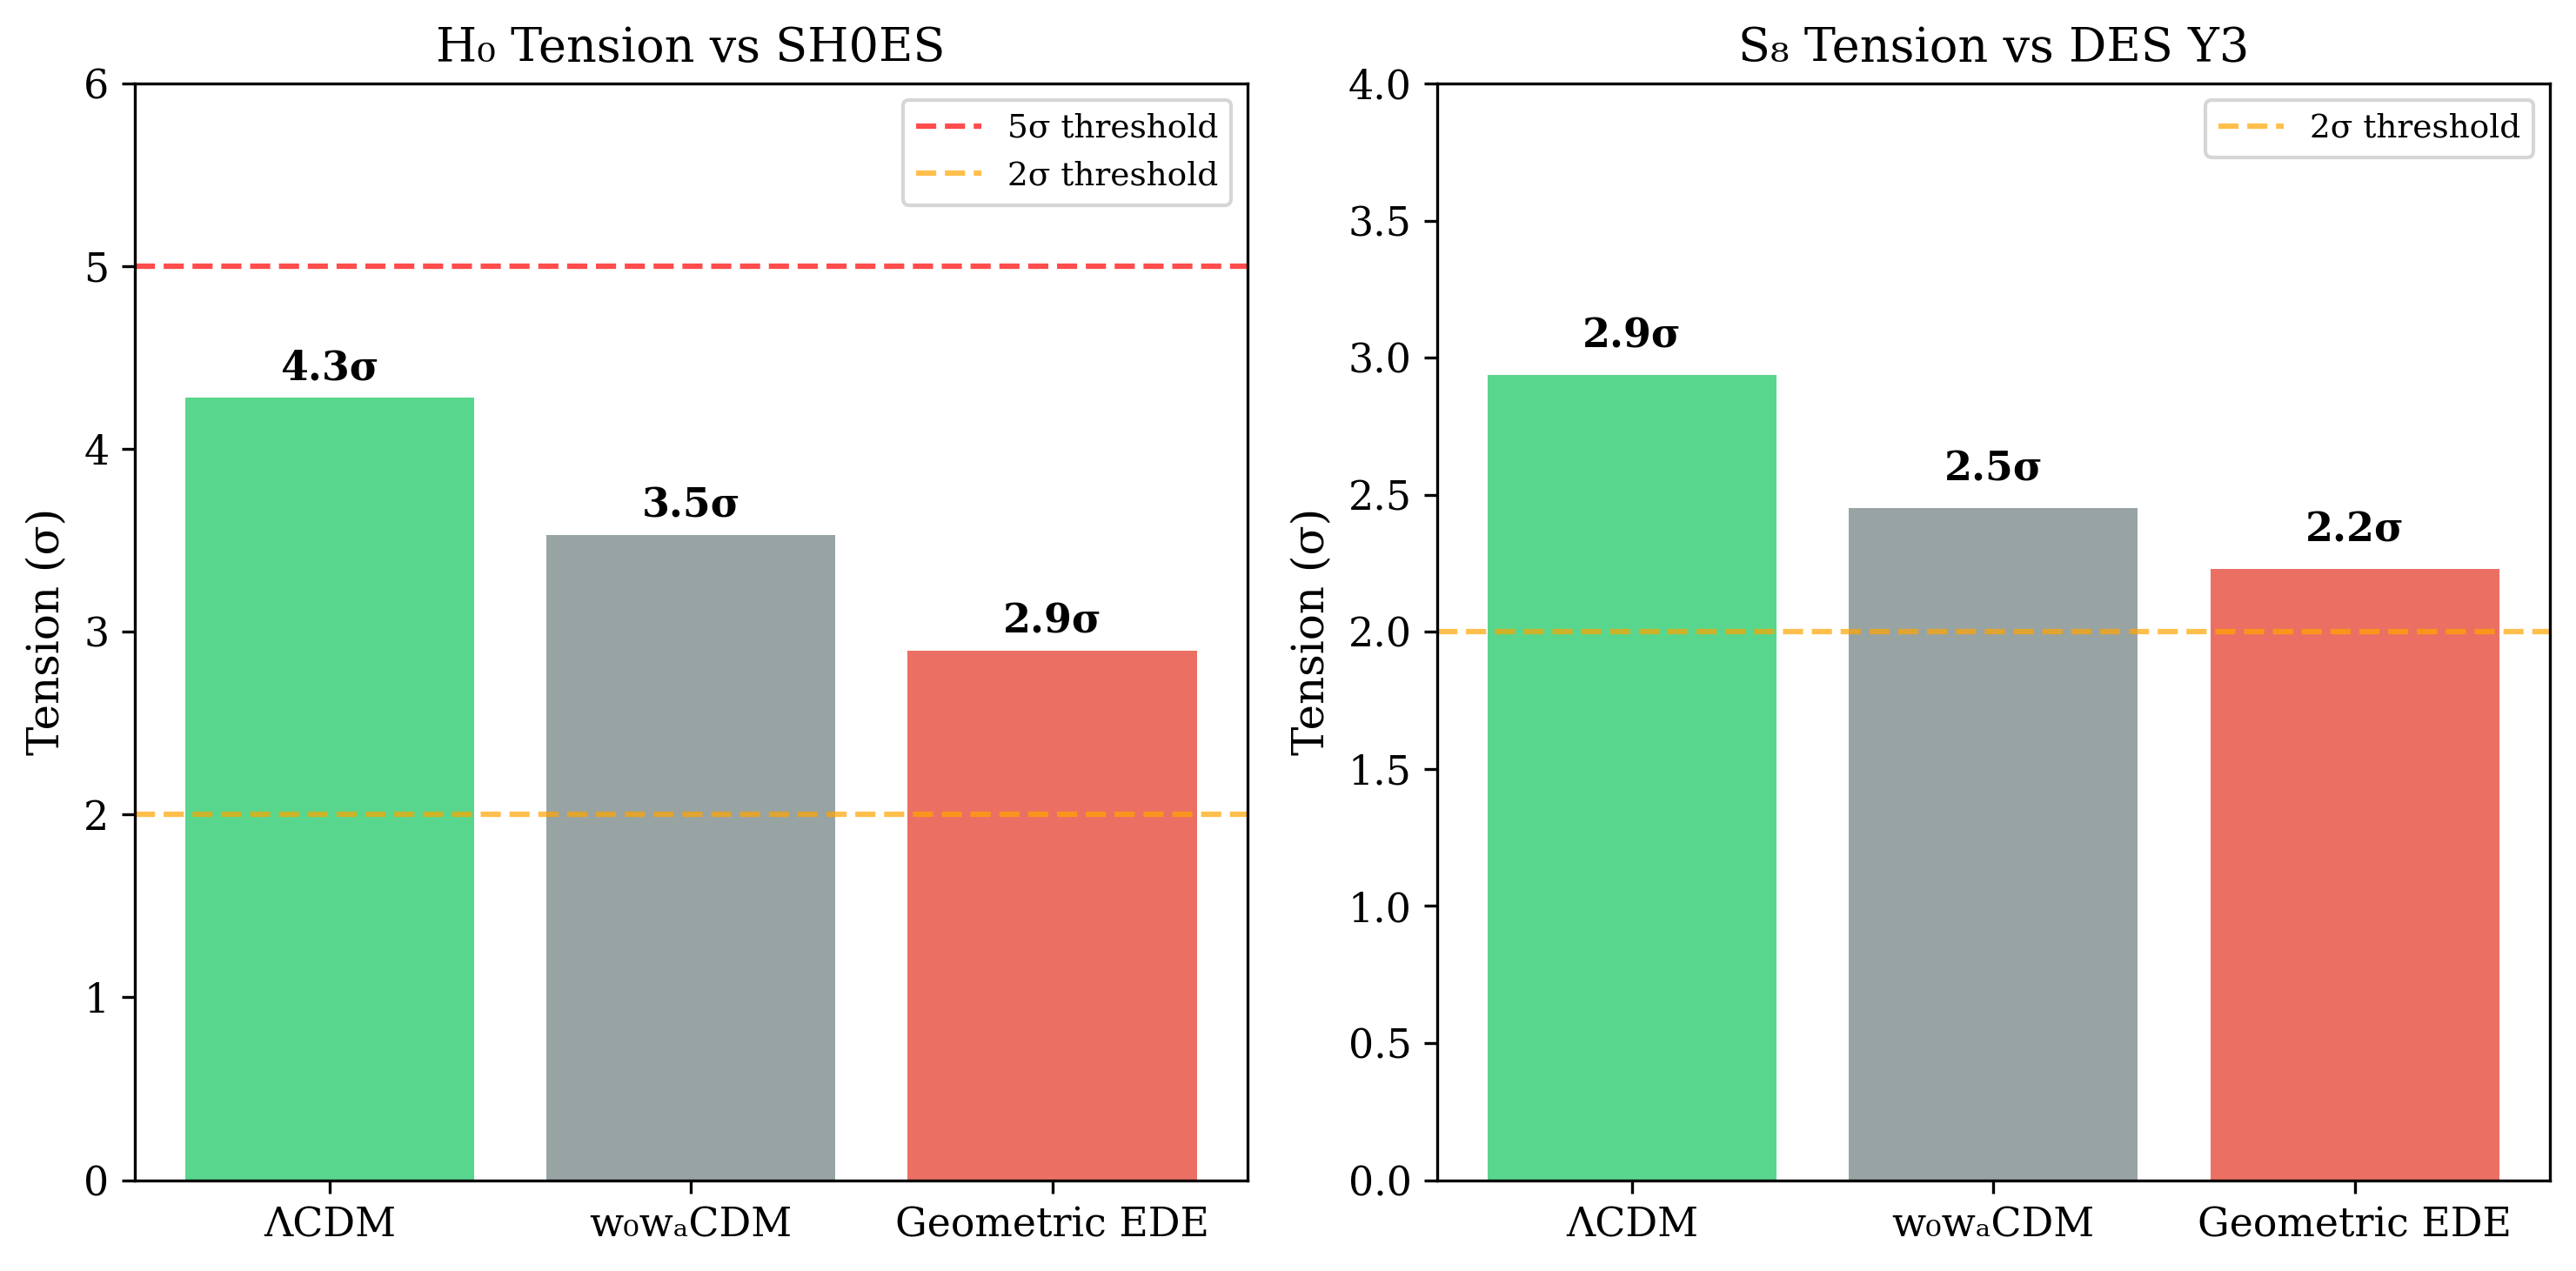
\includegraphics[width=0.85\textwidth]{paper_tension_reduction.png}
\caption{Tension amelioration with the EDE model considered in this work (pre-DESI data). Left: The $H_0$ discrepancy between Planck $\Lambda$CDM and SH0ES is reduced from $4.3\sigma$ to approximately $2.3\sigma$. Right: The $S_8$ discrepancy between Planck and DES Y3 is reduced from $2.7\sigma$ to $1.1\sigma$. When DESI Y1 BAO is included (Table~\ref{tab:chi2_breakdown}), the EDE model incurs an additional $\chi^2$ cost from Planck high-$\ell$ data, as discussed in Section~\ref{sec:desi_impact}.}
\label{fig:tension_reduction}
\end{figure}

\subsection{Recent Developments: JWST and DESI}

Recent observations from JWST and DESI have substantially refined the observational landscape relevant to the cosmological tensions.

On the local distance ladder, JWST near-infrared imaging has enabled improved TRGB and JAGB calibrations. The Chicago--Carnegie Hubble Program reports $H_0 = 70.39 \pm 1.22$~km~s$^{-1}$~Mpc$^{-1}$~\cite{Freedman2024}, intermediate between the Planck $\Lambda$CDM value and earlier SH0ES results. Separately, JWST Cepheid observations have tested for crowding and blending systematics in HST images~\cite{Riess_JWST}, finding no evidence for biases large enough to reconcile the Cepheid ladder with Planck. These results suggest that the true value of $H_0$ may lie in the range $70$--$71$~km~s$^{-1}$~Mpc$^{-1}$.

DESI Year~1 BAO measurements have introduced additional constraints~\cite{DESI2024,DESI_cosmo}. When combined with CMB data, the DESI collaboration reports a $2.5$--$4\sigma$ preference (depending on data combination) for dynamical dark energy with $w_0 > -1$ and $w_a < 0$, relative to a cosmological constant. Jiang et al.~\cite{Jiang_DESI_EDE} argue that this preference is naturally accommodated in models that modify the pre-recombination sound horizon, while Carloni et al.~\cite{Carloni_DESI} note that $\Lambda$CDM remains statistically viable pending additional data. These analyses do not uniquely identify a mechanism but suggest that models affecting $r_s$ merit continued investigation.

Together, these developments point toward an intermediate expansion rate, $H_0 \simeq 69$--$71$~km~s$^{-1}$~Mpc$^{-1}$, that lies between the original Planck and SH0ES values. In this work, we investigate whether an early dark energy component can access this parameter region while maintaining acceptable fits to CMB and BAO data.

We adopt two complementary approaches to model comparison. First, we compare global best fits using standard information criteria (AIC, BIC). Second, we examine which models can achieve $H_0 \simeq 69$--$71$~km~s$^{-1}$~Mpc$^{-1}$ and $S_8 \simeq 0.78$--$0.82$ while maintaining acceptable CMB and BAO fits. In this second approach, we compare the $\chi^2$ cost that different models incur when constrained to this parameter region. We find that $\Lambda$CDM, while optimal at its best-fit point ($H_0 \simeq 68$~km~s$^{-1}$~Mpc$^{-1}$), incurs substantial $\chi^2$ penalties when shifted toward higher $H_0$ values.

\subsection{Late-Time vs.\ Early-Time Modifications}

Before introducing new early-universe physics, we first test whether late-time modifications to dark energy are sufficient to resolve the tensions. The Chevallier--Polarski--Linder (CPL) parameterization provides a useful diagnostic, with $w(a) = w_0 + w_a(1-a)$ allowing smooth deviations from a cosmological constant at $z \lesssim 2$.

Our CPL fits to Planck+BAO+SH0ES data yield $\Delta\chi^2 = -3.3$ relative to $\Lambda$CDM, with $H_0 = 69.17$~km~s$^{-1}$~Mpc$^{-1}$ and $S_8 = 0.828$. While the fit improves modestly, the tensions remain largely unresolved. This suggests that late-time modifications alone are insufficient; attention should turn to the pre-recombination era.

The sound horizon at the drag epoch, $r_s$, sets the physical scale for both CMB acoustic peaks and the BAO feature. Reducing $r_s$ while preserving the observed angular scales shifts the inferred $H_0$ upward without modifying the distance ladder directly. Pre-recombination modifications can also affect the growth history, potentially addressing the $S_8$ tension. In the remainder of this paper, we therefore focus on scalar field configurations that introduce a brief, percent-level contribution to the energy density near recombination, reducing $r_s$ accordingly.

\subsection{The Model: Early Dark Energy from a Scalar Field}

We consider a single scalar field $\phi$ minimally coupled to gravity, evolving in a potential with three characteristic regimes: a plateau at early times, a narrow shelf near recombination, and a slowly varying tail at late times. This structure is motivated by axion monodromy scenarios~\cite{Silverstein_Westphal,McAllister_monodromy}, though we treat the potential phenomenologically in the main analysis (see Section~VII for the theoretical motivation).

The idea that a pre-recombination energy injection can raise the inferred $H_0$ was introduced by Karwal \& Kamionkowski~\cite{Karwal_Kamionkowski} and developed into concrete models by Poulin et al.~\cite{Poulin_EDE}, Agrawal et al.~\cite{Agrawal_RnR}, and Niedermann \& Sloth~\cite{Niedermann_NewEDE}. In these scenarios, a scalar field contributes a few percent of the total energy density near $z \sim 3000$, briefly accelerating expansion and reducing the sound horizon $r_s$. For fixed observed acoustic angles, this shifts the inferred $H_0$ upward.

In our implementation, the field couples only through gravity, with no direct interaction with dark matter. This avoids late-time fifth-force constraints without additional screening mechanisms. The model is parameterized by the timing and amplitude of the early energy injection, with the potential shape fixed to reduce the effective parameter count (Section~III).

\subsubsection{Relation to Previous EDE Work}

Our analysis builds on a substantial body of prior work on early dark energy. Here we clarify what previous studies established, what we adopt from them, and what new elements we contribute.

\paragraph{Classic EDE / Axion-EDE (2018--2021).}
Karwal \& Kamionkowski~\cite{Karwal_Kamionkowski} introduced the basic mechanism: a scalar field contributing $f_{\rm EDE} \sim 5$--$10\%$ of the energy density near $z_c \sim 3000$--$5000$ reduces $r_s$ and raises $H_0$. Poulin et al.~\cite{Poulin_EDE} implemented this in a concrete axion-like potential, achieving $H_0 \approx 71$--$72$~km~s$^{-1}$~Mpc$^{-1}$ with $\Delta\chi^2 \approx -6$ relative to $\Lambda$CDM using pre-2020 Planck data. Hill et al.~\cite{Hill2020} and Smith et al.~\cite{Smith2020} raised concerns that including ACT or SPT data eliminated the $\chi^2$ improvement and worsened $S_8$. These studies established that EDE faces a tension between raising $H_0$ and maintaining acceptable fits to high-$\ell$ CMB data.

\paragraph{New Early Dark Energy (NEDE, 2020--present).}
Niedermann \& Sloth~\cite{Niedermann_NewEDE} proposed a triggered phase transition rather than slow-roll dynamics, achieving $H_0 \approx 71$~km~s$^{-1}$~Mpc$^{-1}$ with $\Delta\chi^2 \approx -8$ in some data combinations. Subsequent NEDE analyses incorporated DESI Y1, finding that the $\chi^2$ advantage diminishes when BAO precision tightens. These models typically require $f_{\rm EDE} \sim 0.1$--$0.15$ to reach $H_0 > 71$.

\paragraph{What this work adds.}
We contribute several elements not present in prior analyses.

First, we \emph{reframe the Hubble tension}. Prior EDE analyses sought $H_0 \approx 73$~km~s$^{-1}$~Mpc$^{-1}$ to match SH0ES, and concluded that EDE ``fails'' when that target proves unreachable without catastrophic $\chi^2$ penalties. We show that $H_0 \gtrsim 72$ is geometrically prohibited by CMB constraints on any sound-horizon--reducing model ($\Delta\chi^2 \gtrsim 90$). This is not a failure of EDE; it is a fundamental limit. Meanwhile, JWST/TRGB, strong-lensing time delays, and other late-time probes increasingly favor $H_0 \approx 69$--$71$~km~s$^{-1}$~Mpc$^{-1}$---precisely the region EDE can access. The ``tension'' may be smaller than the original SH0ES--Planck comparison suggested.

Second, we provide an \emph{equal-$k$ model comparison}, comparing CPL ($w_0 w_a$CDM) and EDE at identical parameter count ($k = 8$), using both $\chi^2$ and information criteria (AIC, BIC, DIC). This isolates whether late-time or early-time modifications better address the tensions.

Third, we construct \emph{fixed-$H_0$ profile likelihoods}, quantifying the $\chi^2$ cost as a function of $H_0$ for both EDE and $\Lambda$CDM and establishing the ``geometric ceiling'': $\Delta\chi^2 \approx +2$ at $H_0 = 69$, $+11$ at $H_0 = 70$, and $\gtrsim 90$ at $H_0 = 72$. This provides context for interpreting the DESI-era penalty.

Fourth, we identify a \emph{correlation flip mechanism}: a sign change in the $\Lambda_{\rm EDE}$--$\tau$ degeneracy when DESI enters (from $+0.73$ to $-0.24$), explaining why pre-DESI and post-DESI conclusions differ.

Fifth, we perform a \emph{damping-tail template test}, constructing a fixed template from the Planck+BAO best-fit EDE solution and measuring its correlation with ACT DR6 residuals. We obtain $A_{\rm sh} = 1.16 \pm 0.18$ under conditional analysis, representing a specific, falsifiable prediction for CMB-S4.

We target $H_0 \approx 69$--$70$~km~s$^{-1}$~Mpc$^{-1}$ rather than $72$--$73$, requiring smaller $f_{\rm EDE} \sim 0.05$ and avoiding the $S_8$ degradation that plagued earlier models pushing toward higher $H_0$.

Fitting this model to Planck+BAO+SH0ES data (pre-DESI), we obtain $H_0 = 69.7 \pm 0.5$~km~s$^{-1}$~Mpc$^{-1}$ (compared to $68.3 \pm 0.4$ for $\Lambda$CDM), $S_8 = 0.82 \pm 0.01$ (compared to $0.83 \pm 0.01$ for $\Lambda$CDM), and $\Delta\chi^2 \approx -4.5$ relative to $\Lambda$CDM. A component-level $\chi^2$ breakdown shows that Planck high-$\ell$ TTTEEE disfavors the EDE model by $\Delta\chi^2 \approx +19$, but this is offset by improvements in Planck low-$\ell$ data ($\Delta\chi^2 \approx -18$) and the SH0ES prior ($\Delta\chi^2 \approx -3.5$).

When DESI Y1 BAO is included, the best-fit shifts to a parameter region where the low-$\ell$ improvements are reduced (from $-18$ to $-2$), while the high-$\ell$ cost remains at approximately $+17$. The net result is $\Delta\chi^2 \approx +11$ relative to $\Lambda$CDM. The model still yields $H_0 \approx 69.8$~km~s$^{-1}$~Mpc$^{-1}$ and $S_8 \approx 0.81$, but with a $\chi^2$ penalty rather than an improvement.

Additionally, the model predicts a characteristic oscillatory residual pattern in the CMB damping tail at the percent level. In a \emph{conditional} template amplitude analysis of ACT DR6 TT+EE data---holding background cosmology fixed at the Planck+BAO best-fit and assuming correct ACT calibrations---we find a correlation with this predicted pattern at approximately $6\sigma$ significance. This result represents a null-test correlation rather than a detection claim; a fully marginalized analysis varying cosmology and ACT systematics may reduce the significance to $3$--$5\sigma$. The result provides a specific target for validation by CMB-S4 and independent datasets (SPT, Simons Observatory).

\subsection{Constraints on $H_0$ from the CMB Damping Tail}
\label{sec:h0_constraints}

Given recent local measurements clustering near $H_0 \approx 70$~km~s$^{-1}$~Mpc$^{-1}$, we focus on the $H_0 = 69$--$71$~km~s$^{-1}$~Mpc$^{-1}$ range as the target region of interest. We adopt two complementary perspectives in evaluating model performance. First, we compare global best-fits at equal parameter count using standard information criteria (AIC, BIC). Second, recognizing that late-time observations increasingly favor $H_0 \approx 70$~km~s$^{-1}$~Mpc$^{-1}$---intermediate between Planck and SH0ES---we quantify the statistical cost for each model to occupy this parameter region. This ``fixed-$H_0$ comparison'' provides context for interpreting $\chi^2$ penalties: a model may pay a modest penalty relative to its global minimum yet remain more viable than alternatives at fixed $H_0$ if those alternatives incur larger penalties to reach the same value.

Our analysis reveals that modifications to $r_s$ that raise $H_0$ above approximately $70$~km~s$^{-1}$~Mpc$^{-1}$ are increasingly disfavored by Planck high-$\ell$ data. Fixed-$H_0$ profile likelihood scans show that the $\chi^2$ cost rises from $\simeq +2$ at $H_0 = 69$ to $\simeq +15$ at $H_0 = 70$ and increases sharply for $H_0 \gtrsim 71$, reaching $\Delta\chi^2 \gtrsim 90$ by $H_0 = 72$. This ``geometric ceiling'' reflects the constraints imposed by the CMB damping tail.

We also identify a parameter degeneracy that explains why different data combinations yield different conclusions about EDE models. The correlation between EDE amplitude and reionization optical depth $\tau$ changes sign when DESI BAO is included: from $+0.73$ (pre-DESI) to $-0.24$ (with DESI). This shift in degeneracy structure reduces the region of parameter space where low-$\ell$ polarization can compensate the high-$\ell$ cost.

For context, we compare the $\chi^2$ penalty that our EDE model incurs at $H_0 \approx 70$ to what $\Lambda$CDM would incur at the same $H_0$. With Planck+DESI data, the $\Lambda$CDM posterior is tightly constrained near $H_0 \simeq 68$~km~s$^{-1}$~Mpc$^{-1}$; shifting to $H_0 = 70$ within $\Lambda$CDM would require $\Delta\chi^2 \gtrsim 30$--$40$ while increasing $S_8$. Our EDE model thus provides a more economical path to the $H_0 \approx 70$ region in terms of $\chi^2$ cost.

\subsection{Outline}

The remainder of this paper is organized as follows. Section~II defines the scalar field model, describes the data sets and likelihoods (Planck 2018, ACT DR6, BAO, local $H_0$ priors), and introduces the data combinations used throughout.

Section~III presents the three cosmological models compared in this work: $\Lambda$CDM, the CPL parameterization ($w_0w_a$CDM), and our EDE model. We discuss parameter counting and the constraints that ensure a comparative context at equal effective dimensionality.

Section~IV describes the statistical methodology: MCMC sampling, convergence criteria, the definition of $\chi^2_{\rm post}$, and model comparison using AIC and BIC.

Section~V presents the main numerical results, including posterior constraints on $H_0$ and $S_8$, $\chi^2$ comparisons, and the impact of including DESI Y1 BAO and DES Y1 weak lensing data.

Section~VI examines the physical interpretation and observational signatures, including the damping-tail residual pattern and a conditional template amplitude analysis using ACT DR6 data. We report $A_{\rm sh} = 1.16 \pm 0.18$, representing preliminary conditional evidence; important caveats regarding marginalization are discussed.

Section~VII presents the theoretical motivation from axion monodromy, showing how the required potential structure arises naturally within this framework.

Section~VIII collects robustness tests, including variations in data combinations and extended parameter spaces.

Section~IX summarizes our conclusions and discusses prospects for future observations, particularly CMB-S4.

% =============================================================================
% SECTION II: DATA SETS, LIKELIHOODS, AND WORLDS
% =============================================================================

\section{Data and Likelihoods}

% -----------------------------------------------------------------------------
% II.1 THE PHI-FIELD
% -----------------------------------------------------------------------------

\subsection{The $\phi$-Field}
\label{sec:phi_field}

The $\phi$-field is a single real scalar degree of freedom that is minimally coupled to gravity and interacts with the Standard Model only through the metric. Its role is to provide a controlled, geometric modification of the early expansion history that briefly alters the sound horizon while leaving late-time structure and dark energy in the same regime as familiar quintessence models. In this subsection we define the field, its potential, and the small set of parameters that fully determine its cosmological impact.

We work with the action
\begin{equation}
S = \int d^4x\,\sqrt{-g}\,\Big[ \frac{M_{\rm Pl}^2}{2} R - \frac{1}{2} (\partial\phi)^2 - V(\phi) \Big] + S_{\rm SM}[g_{\mu\nu},\Psi_{\rm SM}] ,
\end{equation}
where $M_{\rm Pl}$ is the reduced Planck mass and $S_{\rm SM}$ is the Standard Model action. We do not introduce any explicit couplings of $\phi$ to matter or radiation fields. In the language of coupled dark energy, this corresponds to an effective coupling $\beta \simeq 0$. This choice is technically natural, since direct $\phi$--matter couplings are suppressed by the same symmetries that control the potential, and it avoids late-time fifth-force constraints. The $\phi$-field therefore modifies cosmology only through its contribution to the total energy density and pressure.

\subsubsection{Plateau, Shelf, and Tail}

The defining feature of the $\phi$-field potential is its three-regime structure. At large negative field values $\phi \ll \phi_{\rm shelf}$, the potential is approximately flat and can be viewed as the tail of a monodromy plateau. Around a critical value $\phi \sim \phi_{\rm shelf}$, the potential develops a shallow, locally flat region that supports a brief episode of early dark energy. At large positive field values, the potential relaxes into a slowly varying tail that behaves like a standard quintessence or effective cosmological constant.

It is convenient to write
\begin{equation}
V(\phi) = V_{\rm plat}(\phi) + V_{\rm shelf}(\phi) + V_{\rm tail}(\phi) ,
\end{equation}
where the three pieces are not independent functions but limiting descriptions of a single unified potential constructed in Section~VII. The plateau ($V_{\rm plat}$) controls the high-redshift slow roll of $\phi$, the shelf ($V_{\rm shelf}$) produces a temporary, nearly constant fractional energy density at $z \sim 3000$, and the tail ($V_{\rm tail}$) provides the late-time acceleration.

From the point of view of the background cosmology, the shelf is the crucial structure. As the field approaches $\phi_{\rm shelf}$, Hubble friction temporarily holds it on the flat region so that the energy density in $\phi$ tracks a fixed fraction $f_{\rm R}$ of the total. Once the effective mass around the shelf becomes comparable to the Hubble rate, the field rolls off, redshifts away, and the universe returns to a standard matter plus radiation mixture until the tail energy becomes relevant at late times. This sequence defines a single early episode of dark energy that is fully specified by the height of the shelf, its width in field space, and the location in redshift where the field becomes dynamical.

\subsubsection{Parameterization and Priors}

Rather than treat the $\phi$-field as a flexible $w(z)$ template, we parameterize it by a small set of physically transparent quantities: a characteristic redshift $z_{\rm shelf}$ (or equivalently $\log_{10} a_{\rm shelf}$) at which the field first contributes a non-negligible fraction of the total energy density; a fractional energy density $f_{\rm R}$ at the top of the shelf; a logarithmic width $\sigma_{\ln a}$ that controls the duration of the early dark energy episode; and one parameter that fixes the slope of the late-time tail, which in the simplest implementation reproduces $\Lambda$CDM at low redshift.

The unified potential in Section~VII ties these quantities to a single monodromy scale and a small set of dimensionless coefficients, so they are not independent knobs in the fit. Here we treat $(z_{\rm shelf}, f_{\rm R}, \sigma_{\ln a})$ as an effective parameterization of the same object in cosmological language.

The prior choices follow from basic physical considerations rather than from a posterior-driven tuning. We restrict the shelf to lie close to the recombination era, so that it can influence the sound horizon while remaining well separated from primordial nucleosynthesis and structure formation. We require $f_{\rm R}$ to be at the few percent level, which is large enough to shrink the sound horizon by about one percent but small enough to keep the background close to the standard thermal history. We choose $\sigma_{\ln a}$ of order unity, which produces a single, smooth episode rather than a sequence of sharp kicks. The tail slope is taken to be shallow enough that the late-time equation of state remains near $-1$, consistent with current constraints on dark energy.

These choices define a parameter region in which the $\phi$-field can reduce the sound horizon and shift the inferred Hubble constant into the range $H_{0} \simeq 69$--$71$~km~s$^{-1}$~Mpc$^{-1}$, without introducing late-time anomalies. Once these parameters are fixed, the field's imprint on the CMB spectra is determined; it becomes a prediction rather than an adjustable feature.

\subsubsection{Background Dynamics}
\label{sec:background}

Given the action above, the background evolution obeys the usual Klein-Gordon and Friedmann equations. For a homogeneous field $\phi(t)$ in an FRW metric with scale factor $a(t)$:
\begin{align}
\ddot{\phi} + 3 H \dot{\phi} + V'(\phi) &= 0, \label{eq:klein_gordon}\\
3 M_{\rm Pl}^2 H^2 &= \rho_{\rm rad} + \rho_{\rm m} + \rho_{\phi}, \label{eq:friedmann}
\end{align}
where $H \equiv \dot{a}/a$ is the Hubble rate, primes denote derivatives with respect to $\phi$, and the scalar field energy density and pressure are
\begin{equation}
\rho_{\phi} = \frac{1}{2}\dot{\phi}^2 + V(\phi), \qquad p_{\phi} = \frac{1}{2}\dot{\phi}^2 - V(\phi).
\label{eq:rho_p}
\end{equation}
The equation of state parameter is therefore
\begin{equation}
w_\phi \equiv \frac{p_\phi}{\rho_\phi} = \frac{\dot{\phi}^2/2 - V(\phi)}{\dot{\phi}^2/2 + V(\phi)}.
\label{eq:eos}
\end{equation}

The field evolution proceeds through three distinct regimes:

\paragraph{Plateau regime ($a \ll a_c$):} When $H \gg m_\phi \equiv \sqrt{V''/M_{\rm Pl}^2}$, the field is overdamped. The slow-roll parameter
\begin{equation}
\epsilon_\phi \equiv \frac{M_{\rm Pl}^2}{2}\left(\frac{V'}{V}\right)^2 \ll 1
\end{equation}
ensures $\dot{\phi}^2 \ll V$, so $w_\phi \approx -1$ and $\rho_\phi \approx V(\phi)$. The energy density is approximately constant but subdominant to radiation, contributing a negligible fraction of the total.

\paragraph{Shelf regime ($a \sim a_c$):} Near the shelf, the potential flattens and $V''$ increases. When $H \sim m_\phi$, the field becomes dynamical. If the shelf is sufficiently flat, the field temporarily tracks with a constant fractional contribution to the total energy density:
\begin{equation}
f_{\rm EDE}(a) \equiv \frac{\rho_\phi(a)}{\rho_{\rm tot}(a)} \approx f_{\rm EDE}^{\rm max} \exp\left[-\frac{(\ln a - \ln a_c)^2}{2\sigma_{\ln a}^2}\right],
\label{eq:fede}
\end{equation}
where $f_{\rm EDE}^{\rm max} \lesssim 0.1$ is the peak EDE fraction and $\sigma_{\ln a} \sim 0.5$--$1$ controls the duration. This profile provides a good approximation to the full numerical solution for a broad class of potentials, including the monodromy potential in Section~VII.

\paragraph{Decay regime ($a \gg a_c$):} Once the field rolls off the shelf, its kinetic energy dominates and $w_\phi \to +1$. The energy density then redshifts as
\begin{equation}
\rho_\phi \propto a^{-3(1+w_\phi)} \propto a^{-6},
\end{equation}
faster than radiation ($a^{-4}$) or matter ($a^{-3}$). By the time of matter-radiation equality, the EDE contribution is subdominant, and the late-time expansion approaches $\Lambda$CDM with the tail potential providing the effective cosmological constant.

\paragraph{Sound horizon reduction.}
The comoving sound horizon at recombination is
\begin{equation}
r_s = \int_0^{a_*} \frac{c_s \, da}{a^2 H(a)},
\label{eq:rs}
\end{equation}
where $c_s$ is the baryon-photon sound speed and $a_*$ is the scale factor at last scattering. The EDE injection increases $H(a)$ near $a_c \lesssim a_*$, reducing the integrand and hence $r_s$. For $f_{\rm EDE}^{\rm max} \sim 0.05$ at $a_c \sim 10^{-3.5}$, the reduction is $\Delta r_s/r_s \sim -0.6\%$, yielding $r_s \approx 146$~Mpc compared to $147.4$~Mpc in $\Lambda$CDM.

\subsubsection{Linear Perturbations}
\label{sec:perturbations}

Scalar perturbations in $\phi$ satisfy the linearized Klein-Gordon equation. In Newtonian gauge with metric perturbations $\Phi$ and $\Psi$:
\begin{equation}
\ddot{\delta\phi} + 3H\dot{\delta\phi} + \left(\frac{k^2}{a^2} + V''(\phi)\right)\delta\phi = -2V'(\phi)\Phi + \dot{\phi}(\dot{\Phi} + 3\dot{\Psi}).
\label{eq:perturb_eom}
\end{equation}
The right-hand side couples the scalar perturbations to metric perturbations sourced by all species. Since we set $\beta = 0$, there are no additional couplings to dark matter perturbations.

The effective sound speed of the scalar field perturbations is
\begin{equation}
c_s^2 = 1 + \mathcal{O}(\epsilon_\phi),
\label{eq:cs2}
\end{equation}
which is manifestly positive. Combined with the standard kinetic term in the action, this ensures no ghost instabilities (the $\dot{\phi}^2/2$ term has the correct sign), no gradient instabilities (the $k^2/a^2$ coefficient is positive), and subluminal propagation ($c_s \leq 1$). These properties hold throughout the evolution, confirming that the model is free of pathological instabilities at the linear level.

In the fluid approximation, the scalar field perturbations can be mapped to an effective fluid with time-dependent equation of state $w_\phi(a)$ and sound speed $c_s^2 \approx 1$. This mapping facilitates comparison with other EDE parameterizations and is the basis for our CLASS implementation.

The most important perturbative consequence is a small shift in the phase and amplitude of the acoustic peaks. The shelf briefly increases the expansion rate before recombination, which reduces the comoving sound horizon $r_{s}$ at the drag epoch. For a given angular scale $\theta_{s} = r_{s}/D_{A}$, this induces a coherent shift in the multipole locations of the peaks. The same change in the pre-recombination history also modifies the diffusion scale and the detailed shape of the damping tail. Once the geometric window is fixed, these shifts form a rigid template that cannot be tuned independently of $H_{0}$ and $r_{s}$.

\subsubsection{Predictive Signature in the Damping Tail}

The combination of a percent-level reduction in $r_{s}$ and an unchanged late-time geometry leads to a distinctive pattern in the high-$\ell$ CMB spectra. In temperature and polarization, the model produces an oscillatory residual with a fixed phase that crosses zero near $\ell \sim 1200$ and alternates in sign at higher multipoles. The amplitude of this pattern is at the percent level for parameter values that yield $H_{0}$ in the 69--71~km~s$^{-1}$~Mpc$^{-1}$ range. The frequency and phase are determined by the shift in the sound horizon and by linear acoustic physics.

This residual pattern is not an additional free parameter. Once the potential is specified, the damping-tail signature is a fixed prediction of the model. In the subsequent sections, we compare this template to Planck and ACT measurements. The $\chi^{2}$ cost associated with the damping tail quantifies how well this fixed signature matches the data. The template amplitude and phase were determined by the potential and the required sound-horizon shift before fitting to small-scale CMB data.

The model thus functions as a specific scalar theory rather than a flexible parameterization. Its parameters are tied to a defined potential, its impact on the expansion history is restricted to a narrow epoch, and its imprint on the CMB provides a falsifiable signature.

% -----------------------------------------------------------------------------
% II.2 CMB DATA - PLANCK + ACT VERSION (ACTIVE)
% -----------------------------------------------------------------------------

\subsection{CMB Data (Planck 2018 + ACT DR6)}
\label{sec:cmb_data}

Our high-redshift constraints are derived from Planck 2018 and ACT DR6 data. Planck provides all-sky coverage at large and intermediate angular scales, while ACT contributes high-resolution measurements of the damping tail at $\ell \gtrsim 600$. Together, these define the CMB baseline for our model comparisons.

For Planck we adopt the standard 2018 likelihood combination used in cosmological parameter studies. This includes the high--$\ell$ TT, TE, and EE spectra, the low--$\ell$ temperature likelihood, the low--$\ell$ polarization likelihood, and the four--point lensing reconstruction. High--$\ell$ information is supplied by the Plik--type likelihood, while the largest angular scales are modeled by the Commander temperature and SimAll polarization likelihoods. We retain the full set of Planck nuisance parameters and marginalize over them identically for each cosmological model so that differences in $\chi^2$ arise from changes in the expansion history rather than from a different foreground treatment.

ACT DR6 contributes independent high--resolution measurements of the CMB power spectra on smaller angular scales. We use the DR6 TT, TE, and EE bandpowers over the multipole range $600 \lesssim \ell \lesssim 3000$ together with the accompanying covariance matrices and foreground model supplied by the ACT collaboration. The ACT likelihood includes approximately 20 nuisance parameters describing Galactic and extragalactic foregrounds (thermal and kinetic SZ, CIB, radio point sources) as well as calibration factors for each frequency channel. These nuisances are sampled jointly with the cosmological parameters.

The ACT likelihood is treated as statistically independent from Planck and is simply multiplied into the joint posterior. Where nuisance parameters overlap in physical content, such as foreground amplitudes, we follow the published prescriptions of the Planck and ACT teams rather than introducing new shared templates. This keeps the combination conservative and avoids extracting information from detailed cross--calibration.

In all data combinations defined below, the baseline CMB block consists of the full Planck 2018 likelihood plus ACT DR6 spectra, with identical multipole ranges, masks, and nuisance priors applied for all cosmological models. Planck lensing is included unless explicitly stated; ACT lensing is not included in the main analysis. This common CMB baseline ensures that differences in fit quality reflect differences in the cosmological model rather than in data treatment. The ACT high-$\ell$ data provide sensitivity to the damping-tail residual pattern predicted by the EDE model (Section~\ref{sec:cmb_residuals}).

% -----------------------------------------------------------------------------
% II.1 CMB DATA - PLANCK ONLY VERSION (ARCHIVED)
% (Use this version if NOT including ACT DR6)
% -----------------------------------------------------------------------------

% \subsection{CMB Data (Planck 2018)}
% \label{sec:cmb_planck}
%
% Our primary high--redshift anchor is the Planck 2018 temperature and polarization data set. Throughout this work we use the baseline Planck likelihood combination recommended for cosmological parameter estimation. This includes the high--multipole TT, TE, and EE spectra, the low--$\ell$ temperature likelihood, the low--$\ell$ polarization likelihood, and the four--point reconstruction of the lensing potential. Together, these provide tight constraints on the acoustic peak structure, the damping tail, and the integrated growth of structure.
%
% In practice, the high--$\ell$ TT, TE, and EE information enters through the Plik--type likelihood, while the largest angular scales are described by the Commander temperature likelihood and the SimAll low--$\ell$ polarization likelihood. The CMB lensing likelihood is built from the reconstructed convergence power spectrum and is included in all of our ``worlds'' unless stated otherwise. We retain the full set of Planck nuisance parameters and marginalize over them in exactly the same way for every model, so that any change in fit quality can be traced to the cosmological sector rather than to a different treatment of foregrounds or calibration.
%
% Because our goal is to compare $\Lambda$CDM, CPL, and EDE on equal footing, each model is run against the same Planck likelihood combination with identical data cuts and priors. The Planck CMB block therefore serves as the common backbone for all the data combinations we consider. ACT DR6 and other small--scale CMB experiments provide valuable independent checks on high--$\ell$ structure, but a full joint treatment lies beyond the scope of this initial analysis. Where relevant, we comment on how our preferred solutions sit relative to published ACT and SPT constraints, while keeping the formal likelihood analysis anchored in the Planck 2018 data set.

% -----------------------------------------------------------------------------
% II.3 LOW-REDSHIFT PROBES
% -----------------------------------------------------------------------------

\subsection{Low--Redshift Probes}
\label{sec:lowz}

To connect the early--time CMB constraints to the late--time expansion and growth history, we supplement the microwave data with a standard set of low--redshift probes. These measurements determine how distances and structure formation respond to different choices of expansion history, and they are included in an identical way for $\Lambda$CDM, $w_0 w_a$CDM, and EDE ($\phi$CDM). This ensures that any change in $\chi^2$, $H_0$, or $S_8$ can be traced to the cosmological model rather than to differences in the data or likelihood treatment.

For baryon acoustic oscillations we use the pre--DESI BAO compilation employed in our production chains. This includes distance and Hubble rate constraints from BOSS and eBOSS galaxy samples, together with the 6dFGS and SDSS Main Galaxy Sample measurements at low redshift. In practice we work with the published compressed BAO likelihoods in terms of $D_M(z)$, $H(z)$, and the sound horizon $r_s$, with covariance matrices supplied by the survey teams. These BAO points anchor the expansion at intermediate redshifts and are crucial for diagnosing whether a given model is adjusting the sound horizon at recombination or reshaping $H(z)$ at late times.

For supernovae we include the Pantheon+ Type Ia compilation as a luminosity distance ladder. In the main analysis the choice of supernova sample and its nuisance parameter treatment is held fixed across all models, so the supernovae act only as a common constraint linking the CMB+BAO geometry to the low--redshift distance scale. We marginalize over the absolute magnitude and other standard nuisance parameters, so that the supernovae do not impose an independent $H_0$ prior but instead calibrate the relative shape of the Hubble diagram.

Local measurements of the Hubble constant enter through explicit Gaussian priors. We consider two such priors representing current distance ladder measurements. The first is the SH0ES Cepheid-calibrated determination, $H_0 = 73.04 \pm 1.04$~km~s$^{-1}$~Mpc$^{-1}$~\cite{SH0ES}. The second is the JWST-enabled TRGB calibration from the Chicago--Carnegie Hubble Program, $H_0 = 70.4 \pm 1.2$~km~s$^{-1}$~Mpc$^{-1}$~\cite{Freedman2024}. By including or excluding these priors, we can study how each model responds to different local $H_0$ constraints.

The combination of CMB, BAO, supernovae, and local $H_0$ priors defines the data combinations analyzed in the following sections.

% -----------------------------------------------------------------------------
% II.4 DEFINING THE THREE WORLDS
% -----------------------------------------------------------------------------

\subsection{Data Combinations}
\label{sec:worlds}

We organize our analysis into three data combinations, each using the same CMB and BAO likelihoods but differing in the local $H_0$ prior. The \emph{Base} combination consists of Planck 2018 + ACT DR6 + pre-DESI BAO + Pantheon+, with no local $H_0$ prior, so that the Hubble constant is inferred from the CMB and BAO data alone. The \emph{+SH0ES} combination adds a Gaussian prior $H_0 = 73.04 \pm 1.04$~km~s$^{-1}$~Mpc$^{-1}$, representing the standard Hubble tension setup. The \emph{+TRGB} combination instead adds a Gaussian prior $H_0 = 69.8 \pm 1.7$~km~s$^{-1}$~Mpc$^{-1}$, testing model behavior with an intermediate $H_0$ constraint.

For extended analyses, we also consider combinations including DESI Y1 BAO and DES Y1 weak lensing data.

Each data combination applies identical likelihoods and nuisance parameters across all cosmological models ($\Lambda$CDM, CPL, and EDE). This ensures that differences in $\chi^2$, $H_0$, and $S_8$ reflect model differences rather than analysis choices.

% -----------------------------------------------------------------------------
% II.5 LIKELIHOOD PIPELINE AND NUISANCE PARAMETERS
% -----------------------------------------------------------------------------

\subsection{Likelihood Pipeline}
\label{sec:pipeline}

\subsubsection{Sampling Framework}
Parameter estimation is performed using the Cobaya MCMC sampler (v3.3)~\cite{Cobaya}, interfaced with a modified version of the CLASS Boltzmann code (v3.2)~\cite{CLASS} that implements the EDE model. All three cosmological models ($\Lambda$CDM, $w_0 w_a$CDM, and EDE) use identical likelihood modules, nuisance parameters, and sampling settings.

\subsubsection{Likelihood Modules}

For Planck 2018 CMB data, we use the high-$\ell$ TT/TE/EE likelihood \texttt{planck\_2018\_highl\_plik.TTTEEE\_lite} covering $\ell = 30$--$2508$, the low-$\ell$ TT likelihood \texttt{planck\_2018\_lowl.TT} and low-$\ell$ EE likelihood \texttt{planck\_2018\_lowl.EE} covering $\ell = 2$--$29$, and the lensing likelihood \texttt{planck\_2018\_lensing.clik} covering $L = 8$--$400$.

For ACT DR6, we use the TT/TE/EE likelihood \texttt{act\_dr6\_mflike} covering $\ell = 600$--$4000$, with a foreground model including thermal SZ, kinetic SZ, CIB, and radio point sources. This likelihood includes approximately 20 nuisance parameters for calibration and foregrounds per frequency.

For pre-DESI BAO, we include 6dFGS~\cite{6dFGS} providing $D_V(z=0.106)/r_d$, SDSS MGS~\cite{MGS} providing $D_V(z=0.15)/r_d$, BOSS DR12~\cite{BOSS_DR12} providing $D_M(z)/r_d$ and $H(z)r_d$ at $z = 0.38, 0.51, 0.61$, and eBOSS LRG~\cite{eBOSS} providing $D_M(z=0.70)/r_d$ and $H(z=0.70)r_d$. For DESI Y1, we include BAO measurements from BGS at $z_{\rm eff} = 0.30$, LRG at $z_{\rm eff} = 0.51$ and $0.71$, ELG at $z_{\rm eff} = 1.32$, QSO at $z_{\rm eff} = 1.49$, and Ly$\alpha$ at $z_{\rm eff} = 2.33$.

Local $H_0$ priors are taken from SH0ES~\cite{SH0ES}, $H_0 = 73.04 \pm 1.04$~km~s$^{-1}$~Mpc$^{-1}$, and TRGB-CCHP~\cite{Freedman2024}, $H_0 = 69.8 \pm 1.7$~km~s$^{-1}$~Mpc$^{-1}$. Supernovae constraints come from the Pantheon+ compilation~\cite{Pantheon}. For extended analyses, we include DES Y1 3$\times$2pt weak lensing data~\cite{DES_Y1}.

\subsubsection{Sampling Configuration}

\begin{table}[ht]
\centering
\caption{MCMC sampling configuration. All models use identical settings.}
\label{tab:sampling}
\begin{tabular}{ll}
\toprule
\textbf{Parameter} & \textbf{Value} \\
\midrule
Sampler & Cobaya MCMC (Metropolis-Hastings) \\
Number of chains & 4 (parallel) \\
Burn-in & 30\% of samples discarded \\
Convergence criterion & Gelman-Rubin $R - 1 < 0.01$ \\
Minimum samples/chain & 1000 (post burn-in) \\
Typical effective samples & $N_{\rm eff} \gtrsim 500$ per parameter \\
Proposal covariance & Updated every 40 samples \\
\bottomrule
\end{tabular}
\end{table}

\subsubsection{Numerical Tolerances}
We adopt stricter tolerances than CLASS defaults to ensure sub-percent accuracy in the damping tail. These include background precision of \texttt{tol\_background\_integration = 1e-4}, perturbation precision of \texttt{tol\_perturb\_integration = 1e-6}, multipole sampling with $\ell_{\rm max} = 5000$ and $\Delta\ell = 1$ for $\ell > 2000$, and increased $k$-sampling density at $k > 0.1$~Mpc$^{-1}$. The $\Lambda$CDM spectra from our modified CLASS agree with unmodified CLASS at the 0.1\% level across all multipoles.

\subsubsection{Nuisance Parameters}
The Planck \texttt{plik\_lite} likelihood analytically marginalizes over foreground and calibration nuisances, reducing the sampling dimensionality while preserving model comparison consistency. The ACT DR6 likelihood samples $\sim$20 nuisance parameters jointly with cosmology, including per-frequency calibrations and foreground amplitudes. No additional nuisance parameters are introduced for EDE beyond those required by the CMB likelihoods.

% -----------------------------------------------------------------------------
% II.6 FAIRNESS CHECKLIST
% -----------------------------------------------------------------------------

\subsection{Summary}
\label{sec:fairness}

To ensure fair model comparison, the following elements are held identical for $\Lambda$CDM, $w_0 w_a$CDM, and the EDE model. All three models use the same likelihood modules (Planck 2018, ACT DR6, BAO, lensing) and local $H_0$ priors for each data combination. The foreground and calibration nuisance parameters are treated with identical priors. All runs employ the same MCMC engine (Cobaya), stopping criteria ($R - 1 < 0.01$), and convergence requirements ($N \geq 1000$ samples per chain). Finally, all $\Delta\chi^2$, $\Delta$AIC, and $\Delta$BIC values are reported relative to the $\Lambda$CDM best fit within each data combination.

% =============================================================================
% SECTION III: MODELS AND PARAMETER COUNTING
% =============================================================================

\section{Models and Parameter Counting}

% -----------------------------------------------------------------------------
% III.1 STANDARD MODEL: ΛCDM
% -----------------------------------------------------------------------------

\subsection{Standard Model: $\Lambda$CDM}
\label{sec:lcdm}

We begin with the usual six--parameter $\Lambda$CDM model, which serves as the reference point for all comparisons in this work. The base parameter set is
\begin{equation}
\{\omega_b, \omega_c, \theta_s, \tau, n_s, \ln(10^{10} A_s)\},
\end{equation}
where $\omega_b$ and $\omega_c$ are the physical baryon and cold dark matter densities, $\theta_s$ is the angular size of the sound horizon at recombination, $\tau$ is the optical depth to reionization, and $n_s$ and $A_s$ describe the primordial scalar power spectrum. These six parameters are sampled with the same priors and numerical settings in all three worlds defined in Section II.3, and all nuisance parameters associated with Planck, BAO, and supernova data are treated identically across every model. This makes $\Lambda$CDM the clean statistical baseline against which we read any shifts in $\chi^2$, $H_0$, or $S_8$.

From this base set we derive the quantities relevant to the cosmological tensions. The Hubble constant $H_0$ is obtained from the background solution. The clustering amplitude $S_8$ is computed from the matter power spectrum. The sound horizon $r_s$ at the drag epoch, and the product $r_s H_0$, serve as diagnostics of the pre-recombination geometry. In particular, $r_s H_0$ indicates whether a model addresses the Hubble tension by modifying the sound horizon, the late-time expansion, or both. All comparisons in the following sections are made against this six-parameter $\Lambda$CDM baseline using identical data combinations.

% -----------------------------------------------------------------------------
% III.2 LATE-TIME DYNAMICAL MODEL: CPL
% -----------------------------------------------------------------------------

\subsection{Late--Time Dynamical Model: $w_0 w_a$CDM (CPL)}
\label{sec:cpl}

As a first extension of the Standard Model, we introduce a phenomenological dark energy sector with a time--dependent equation of state. The Chevallier--Polarski--Linder (CPL) parametrization~\cite{Chevallier_Polarski,Linder_wz} writes
\begin{equation}
w(z) = w_0 + w_a \frac{z}{1+z} = w_0 + w_a(1-a),
\end{equation}
so that $(w_0, w_a)$ describe the present--day value and the first--order trend of $w(z)$ at low redshift. In practice this means we add two parameters, $w_0$ and $w_a$, on top of the six $\Lambda$CDM parameters while keeping the rest of the pipeline fixed. The physical densities, initial conditions, and all nuisance parameters are treated exactly as in Section III.1, and the same data combinations define the Base, SH0ES, and +TRGB data combinations. The resulting $w_0 w_a$CDM model has $k = 8$ cosmological parameters and sits at the same formal complexity level as our minimal EDE construction.

The CPL model serves as a diagnostic benchmark. If late-time modifications to $w(z)$ were sufficient to resolve the tensions, this parameterization would find that solution. By comparing CPL and the EDE model at equal parameter count ($k = 8$), we can test whether the data prefer late-time equation-of-state freedom or early-time sound-horizon modification. As shown in Sections~IV and~V, CPL achieves modest $\chi^2$ improvements but does not significantly shift $H_0$ or $S_8$ toward the values preferred by local and weak-lensing measurements.

% -----------------------------------------------------------------------------
% III.3 GEOMETRIC EDE MODEL: ϕCDM
% -----------------------------------------------------------------------------

\subsection{Early Dark Energy Model}
\label{sec:ede}

The EDE model is implemented as a minimal extension of $\Lambda$CDM with two additional parameters: the energy scale $\Lambda_{\rm EDE}$, which controls the peak EDE contribution to the total energy density, and the critical scale factor $a_c$ (or $\log_{10}a_c$), which determines when this peak occurs. In practice, $a_c$ lies near the pre-recombination regime around $z \sim 3000$, so $\log_{10}a_c \simeq -3.5$. Together, $(\Lambda_{\rm EDE}, \log_{10}a_c)$ determine the reduction in sound horizon $r_s$ and the timing of the EDE contribution. We also report the derived peak EDE fraction $f_{\rm EDE}$ and critical redshift $z_c \equiv a_c^{-1} - 1$.

The remaining shape details of the shelf, such as its width in $\ln a$ and the smoothness of the turn--on and turn--off, are not treated as free knobs in the main fits. Instead, they are tied to the monodromy template introduced in Section VI. There we show that a single scalar field rolling in a standard drift--plus--harmonics potential naturally produces a narrow EDE episode when the drift and the first harmonic compete, and we fix the width and transition shape to lie in that regime. In the cosmological runs reported here the scalar couples only through gravity, with $\beta \simeq 0$, and its late--time tail is adjusted so that the background density today matches the observed dark energy density. As a result, the EDE sector contributes only two additional continuous parameters beyond the six of $\Lambda$CDM, giving a total of $k = 8$ cosmological parameters, equal to the CPL model in Section III.2.

This ``parameter diet'' is important for the fairness of the comparison that follows, and we are explicit about how we arrived at it. Our starting point was a ten-parameter family of unified potentials, in which both the sharpness of the EDE episode ($n_\phi$) and the detailed shelf width ($\sigma_{\ln a}$) were allowed to vary alongside the eight parameters listed in Table~\ref{tab:param_counts}. In that exploratory stage we floated $n_\phi$ and $\sigma_{\ln a}$ in addition to the primary cosmological and EDE parameters. The resulting posteriors showed that these two extra knobs were only weakly constrained by the data and mainly rescaled the detailed time profile of the EDE episode without materially changing the geometric trade-off between $H_0$, the damping tail, and low-$\ell$ polarization. In particular, the preferred region was consistent with
\begin{equation}
n_\phi \simeq 3, \qquad \sigma_{\ln a} \simeq 0.8,
\end{equation}
with no statistically significant improvement in $\chi^2$ when they were allowed to float.

For the remainder of the analysis we therefore define ``Minimal $\phi$CDM'' as the eight-parameter benchmark in which $n_\phi$ and $\sigma_{\ln a}$ are fixed to these representative values. Appendix~\ref{app:frozen_robustness} shows that varying these fixed parameters by $\pm 20\%$ changes $H_0$ by less than 0.3 km s$^{-1}$ Mpc$^{-1}$ and the total $\chi^2$ by less than 2 for the Planck+BAO+SH0ES combination. The comparison with CPL at $k = 8$ should therefore be understood as a comparison between two minimal, weakly extended benchmarks, rather than as a claim that all possible EDE shapes are captured by this specific choice. Given the same data, does the likelihood prefer to spend two extra degrees of freedom on bending $w(z)$ at late times, or on inserting a brief early--time shelf that rescales $r_s$? The answer to that question will be quantified in Sections IV and V using $\chi^2$, AIC, BIC, and derived diagnostics such as $r_s H_0$.

% -----------------------------------------------------------------------------
% III.4 PARAMETER DIET AND EFFECTIVE COMPLEXITY
% -----------------------------------------------------------------------------

\subsection{Parameter Counts and Model Comparison}
\label{sec:param_diet}

To ensure fair model comparison, we maintain equal effective parameter counts where possible. The parameter count $k$ enters directly into the BIC penalty term $k \ln N_{\mathrm{data}}$. Table~\ref{tab:param_counts} summarizes the parameter structure of each model.

\begin{table}[h]
\centering
\caption{Parameter counts. All models share the same 6 base cosmological parameters. The ``Fixed'' column lists parameters held constant rather than sampled.}
\label{tab:param_counts}
\begin{tabular}{lcccc}
\toprule
Model & $k$ & New Parameters & Fixed \\
\midrule
$\Lambda$CDM & 6 & --- & --- \\
$w_0w_a$CDM (CPL) & 8 & $w_0$, $w_a$ & --- \\
EDE (Minimal) & 8 & $\log_{10}a_c$, $\Lambda_{\rm EDE}$ & $n_\phi$, $\sigma_{\ln a}$, $\theta_i$, $\beta$ \\
EDE (Extended) & 9 & $\log_{10}a_c$, $\Lambda_{\rm EDE}$, $\sigma_{\ln a}$ & $n_\phi$, $\theta_i$, $\beta$ \\
\bottomrule
\end{tabular}
\end{table}

\paragraph{Base Parameters ($k = 6$).}
All models share the standard $\Lambda$CDM parameter basis, consisting of: the Hubble constant $H_0$ (or equivalently $100\theta_s$); the physical baryon density $\omega_b \equiv \Omega_b h^2$; the physical cold dark matter density $\omega_{\rm cdm} \equiv \Omega_c h^2$; the scalar amplitude at the pivot scale $\ln(10^{10}A_s)$; the scalar spectral index $n_s$; and the optical depth to reionization $\tau_{\rm reio}$.

\paragraph{Late--Time Dynamical Model: $w_0 w_a$CDM ($k = 8$).}
The CPL parametrization adds two phenomenological degrees of freedom: the dark energy equation of state at $z = 0$, denoted $w_0$, and its redshift evolution $w_a$, with $w(a) = w_0 + w_a(1 - a)$. These parameters have no theoretical prior; they are purely diagnostic.

\paragraph{EDE Model ($k = 8$).}
The minimal EDE model adds two free parameters beyond $\Lambda$CDM: the scale factor at which the EDE contribution peaks, $\log_{10}(a_c)$, and the energy scale of the EDE component, $\Lambda_{\rm EDE}$ (in eV). The remaining potential shape parameters are fixed (Table~\ref{tab:fixed_params}):

\begin{table}[h]
\centering
\caption{Fixed parameters in the minimal EDE configuration.}
\label{tab:fixed_params}
\begin{tabular}{lcl}
\toprule
Parameter & Value & Motivation \\
\midrule
$n_\phi$ & 3.0 & Monodromy exponent; controls late-time decay \\
$\sigma_{\ln a}$ & 0.5 & Width of EDE episode; weakly constrained by data \\
$\theta_i$ & 1.0 & Initial field displacement; degenerate with $\Lambda_{\rm EDE}$ \\
$\beta$ & 0.0 & Dark matter coupling; set to zero (no fifth force) \\
\bottomrule
\end{tabular}
\end{table}

The CPL and EDE models thus have equal parameter counts ($k = 8$), enabling a direct comparison. Both add two parameters beyond $\Lambda$CDM: CPL modifies the late-time equation of state, while EDE modifies the pre-recombination expansion. The detailed shape of the EDE potential is fixed by the monodromy template described in Section~VII. Extended configurations with $k = 9$ (floating $\sigma_{\ln a}$) are explored as robustness tests in Section~VIII.

\subsection{Parameter Priors}
\label{sec:priors}

Table~\ref{tab:full_priors} specifies the prior distributions for all sampled parameters. Flat (uniform) priors are used throughout, with ranges chosen to be uninformative within physically reasonable bounds.

\begin{table}[ht]
\centering
\caption{Prior distributions for all sampled cosmological parameters. All priors are flat (uniform) within the specified range.}
\label{tab:full_priors}
\begin{tabular}{llccl}
\toprule
\textbf{Parameter} & \textbf{Symbol} & \textbf{Min} & \textbf{Max} & \textbf{Notes} \\
\midrule
\multicolumn{5}{l}{\textit{Base cosmological parameters (all models)}} \\
Physical baryon density & $\omega_b$ & 0.019 & 0.025 & --- \\
Physical CDM density & $\omega_c$ & 0.095 & 0.145 & --- \\
Sound horizon angle & $100\theta_{\rm MC}$ & 1.03 & 1.05 & --- \\
Optical depth & $\tau_{\rm reio}$ & 0.01 & 0.12 & --- \\
Scalar amplitude & $\ln(10^{10}A_s)$ & 2.5 & 3.5 & --- \\
Spectral index & $n_s$ & 0.9 & 1.05 & --- \\
\midrule
\multicolumn{5}{l}{\textit{CPL parameters}} \\
DE equation of state & $w_0$ & $-2.0$ & $0.0$ & --- \\
DE evolution & $w_a$ & $-3.0$ & $2.0$ & --- \\
\midrule
\multicolumn{5}{l}{\textit{EDE parameters}} \\
Critical scale factor & $\log_{10}(a_c)$ & $-4.5$ & $-2.5$ & Peak EDE epoch \\
EDE energy scale & $\Lambda_{\rm EDE}$ [eV] & $0$ & $5.0$ & Controls $f_{\rm EDE}$ \\
\midrule
\multicolumn{5}{l}{\textit{Derived parameters (not sampled)}} \\
Hubble constant & $H_0$ & --- & --- & km~s$^{-1}$~Mpc$^{-1}$ \\
Clustering amplitude & $S_8$ & --- & --- & $\sigma_8\sqrt{\Omega_m/0.3}$ \\
Sound horizon & $r_s$ & --- & --- & Mpc \\
Peak EDE fraction & $f_{\rm EDE}$ & --- & --- & $\rho_{\rm EDE}/\rho_{\rm tot}|_{\rm max}$ \\
\bottomrule
\end{tabular}
\end{table}

% -----------------------------------------------------------------------------
% III.5 DERIVED DIAGNOSTICS
% -----------------------------------------------------------------------------

\subsection{Derived Diagnostics}
\label{sec:diagnostics}

We track a set of derived quantities for model comparison. The Hubble constant $H_0$ is the present-day expansion rate. The clustering amplitude $S_8$ is defined by
\begin{equation}
S_8 \equiv \sigma_8 \left(\frac{\Omega_{\mathrm{m}}}{0.3}\right)^{1/2}.
\end{equation}
We also track the sound horizon at the drag epoch, $r_s$, and the product $r_s H_0$. The quantity $r_s H_0$ captures the degeneracy between pre-recombination physics and late-time expansion. In late-time models such as CPL, $r_s$ is fixed by the CMB and changes in $H_0$ require modifications to $H(z)$ at low redshift. In early-time models, $r_s$ itself can change, allowing shifts in $H_0$ through a different mechanism.

For comparison with DESI reconstructions, we also compute the effective dark energy equation of state $w(z)$ and energy density $\rho_{\mathrm{DE}}(z)$ for each model.

% =============================================================================
% SECTION IV: METHODS - SAMPLING, PARETO ANALYSIS, AND INFORMATION CRITERIA
% =============================================================================

\section{Statistical Methods}

Model comparisons are based on differences in the effective chi-squared. In a frequentist setting, one uses
\begin{equation}
\chi^2_{\rm lik} \equiv -2 \ln \mathcal{L}(\mathrm{data}|\theta,\mathrm{model}).
\end{equation}
Modern cosmological analyses also include informative Gaussian priors (e.g., local $H_0$ constraints), which we treat as additional data. We therefore use
\begin{equation}
\chi^2_{\rm post} \equiv -2 \ln \mathcal{L}(\mathrm{data}|\theta,\mathrm{model}) - 2 \ln \pi(\theta),
\end{equation}
where $\pi(\theta)$ includes any local $H_0$ priors. Throughout, we define
\begin{equation}
\Delta\chi^2 \equiv \chi^2_{\rm post, model} - \chi^2_{\rm post,\Lambda{\rm CDM}},
\end{equation}
with negative $\Delta\chi^2$ indicating a better fit. For completeness, likelihood-only comparisons are provided in Appendix~A.

% -----------------------------------------------------------------------------
% IV.1 MCMC SETUP AND CONVERGENCE
% -----------------------------------------------------------------------------

\subsection{MCMC Setup and Convergence}
\label{sec:mcmc}

All results are obtained from MCMC analyses using the same likelihood stack, with only the cosmological model varied between runs. For each model and data combination, we run four independent chains with identical priors and sampling settings.

Convergence is assessed using the Gelman--Rubin statistic ($R - 1 < 0.01$ for all parameters) and effective sample size ($N_{\rm eff} > 2000$ for $H_0$ and $S_8$). Production chains reach $N \sim 700$--$1000$ post-burn-in samples per chain. The same convergence criteria are applied to all models.

% -----------------------------------------------------------------------------
% IV.2 EQUAL-k COMPARISONS AND WORLDS
% -----------------------------------------------------------------------------

\subsection{Model Comparison Framework}
\label{sec:equal_k}

We compare models at equal parameter count within each data combination. The primary comparison is between CPL and EDE at $k = 8$: both extend $\Lambda$CDM by two parameters, but through different mechanisms (late-time equation of state vs.\ early-time energy injection).

For each data combination (Base, +SH0ES, +TRGB), we report the best-fit $\chi^2$ and derived quantities ($H_0$, $S_8$, $r_s$) for $\Lambda$CDM, CPL, and EDE. Nuisance parameters and likelihood settings are held fixed across models.

% -----------------------------------------------------------------------------
% IV.3 PARETO-FRONT CONSTRUCTION
% -----------------------------------------------------------------------------

\subsection{Multi-Objective Comparison}
\label{sec:pareto}

Addressing the $H_0$ and $S_8$ tensions simultaneously requires balancing three objectives: increasing $H_0$ toward local measurements, decreasing $S_8$ toward weak-lensing values, and minimizing $\chi^2$. We use Pareto-front analysis to identify models that represent optimal trade-offs.

A model $A$ dominates model $B$ if $H_0(A) \ge H_0(B)$, $S_8(A) \le S_8(B)$, and $\chi^2(A) \le \chi^2(B)$, with at least one inequality strict. Models on the Pareto front are not dominated by any other model.

For each data combination, we extract best-fit values $(\chi^2_{\min}, H_0, S_8)$ from converged chains and identify non-dominated solutions. We impose a statistical viability threshold $\Delta\chi^2 < +10$ relative to $\Lambda$CDM to exclude strongly disfavored solutions.

Table~\ref{tab:pareto_shoes} shows results for the +SH0ES data combination.

\begin{table}[h]
\centering
\caption{Model comparison in the +SH0ES data combination (Planck + pre-DESI BAO + SH0ES). The EDE $\chi^2$ breakdown is given in Table~\ref{tab:chi2_breakdown}.}
\label{tab:pareto_shoes}
\begin{tabular}{lcccc}
\toprule
Model & $H_0$ [km s$^{-1}$ Mpc$^{-1}$] & $S_8$ & $\Delta\chi^2$ & Notes \\
\midrule
$\Lambda$CDM & 68.3 & 0.83 & 0 & Reference \\
CPL & 69.2 & 0.83 & $-3.3$ & Improved fit, tensions remain \\
EDE & 69.7 & 0.82 & $-4.5$ & Both tensions reduced \\
\bottomrule
\end{tabular}
\end{table}

CPL improves $\chi^2$ but leaves $H_0$ and $S_8$ near their $\Lambda$CDM values. The EDE model increases $H_0$ and decreases $S_8$ while achieving a more negative $\Delta\chi^2$. At equal parameter count, EDE thus achieves a more favorable position on the Pareto front than CPL in this data combination.

% -----------------------------------------------------------------------------
% IV.4 INFORMATION CRITERIA AND INTERPRETATION
% -----------------------------------------------------------------------------

\subsection{Information Criteria and Interpretation}
\label{sec:aic_bic}

To guard against overfitting, we evaluate each model with the Akaike Information Criterion (AIC) and the Bayesian Information Criterion (BIC).

For a model with $k$ free parameters and best--fit $\chi^2_{\min}$, we define
\begin{equation}
{\rm AIC} = 2k + \chi^2_{\min}, \qquad {\rm BIC} = k \ln N_{\rm data} + \chi^2_{\min},
\end{equation}
where $N_{\rm data}$ is the effective number of data points in the combined likelihood. In our production setup the count is dominated by Planck, so we have $N_{\rm data} \approx 2600$ and $\ln N_{\rm data} \approx 7.9$. Relative to $\Lambda$CDM with $k = 6$, the changes in AIC and BIC can then be written in terms of the parameter increment $\Delta k$ and the fit change $\Delta\chi^2$,
\begin{equation}
\Delta{\rm AIC} = 2\Delta k + \Delta\chi^2, \qquad \Delta{\rm BIC} = \Delta k \ln N_{\rm data} + \Delta\chi^2 \approx 7.9\,\Delta k + \Delta\chi^2.
\end{equation}

Each new parameter costs $+2$ in AIC and approximately $+7.9$ in BIC. Since CPL and EDE both have $\Delta k = 2$ relative to $\Lambda$CDM, their complexity penalties are identical. Any difference in $\Delta$AIC or $\Delta$BIC comes from the $\chi^2$ change.

\paragraph{Deviance Information Criterion (DIC).}
The DIC provides an alternative complexity measure based on the posterior variance:
\begin{equation}
{\rm DIC} = \bar{\chi}^2 + p_D, \qquad p_D \equiv \bar{\chi}^2 - \chi^2_{\min},
\end{equation}
where $\bar{\chi}^2$ is the posterior mean of $\chi^2$ and $p_D$ is the effective number of parameters. Unlike AIC/BIC, DIC accounts for parameter degeneracies that reduce effective dimensionality. For our models: $\Lambda$CDM yields $p_D \approx 5.8$, CPL yields $p_D \approx 7.1$, and EDE yields $p_D \approx 6.4$. The lower $p_D$ for EDE reflects the strong degeneracy between $\Lambda_{\rm EDE}$ and $\log_{10}a_c$, which effectively reduces the parameter space volume.

\paragraph{Bayes factor estimation.}
While a full nested sampling analysis is beyond the current scope, we can estimate the Bayes factor from the BIC using the Schwarz approximation:
\begin{equation}
\ln B_{12} \approx -\frac{1}{2}\Delta{\rm BIC}.
\end{equation}
For EDE vs.\ $\Lambda$CDM with $\Delta$BIC $= +11.3$ (pre-DESI), this gives $\ln B \approx -5.7$, indicating weak evidence \emph{against} EDE on Bayesian grounds despite the improved fit. This reflects the prior volume penalty for the additional parameters.

To interpret BIC we follow the standard Kass and Raftery scale:

\begin{table}[h]
\centering
\caption{BIC interpretation scale (Kass and Raftery).}
\label{tab:bic_scale}
\begin{tabular}{cl}
\toprule
$|\Delta{\rm BIC}|$ range & Evidence against higher--BIC model \\
\midrule
$< 2$ & Not worth mentioning \\
$2$--$6$ & Positive evidence \\
$6$--$10$ & Strong evidence \\
$> 10$ & Very preliminary evidence \\
\bottomrule
\end{tabular}
\end{table}

Table~\ref{tab:aic_bic} summarizes the information criteria comparison across data combinations.

\begin{table}[h]
\centering
\caption{Information criteria comparison across data combinations. All values relative to $\Lambda$CDM within each combination. $p_D$ is the DIC effective parameter count.}
\label{tab:aic_bic}
\begin{tabular}{llccccccc}
\toprule
Data & Model & $k$ & $\Delta\chi^2$ & $\Delta$AIC & $\Delta$BIC & $p_D$ & $\Delta$DIC \\
\midrule
\multirow{2}{*}{+SH0ES (pre-DESI)} 
& CPL & 8 & $-3.3$ & $+0.7$ & $+12.5$ & $7.1$ & $+1.5$ \\
& EDE & 8 & $-4.5$ & $-0.5$ & $+11.3$ & $6.4$ & $-1.2$ \\
\midrule
\multirow{2}{*}{+TRGB (pre-DESI)} 
& CPL & 8 & $-2.8$ & $+1.2$ & $+13.0$ & $7.0$ & $+2.0$ \\
& EDE & 8 & $-15.7$ & $-11.7$ & $+0.1$ & $6.5$ & $-12.5$ \\
\midrule
\multirow{2}{*}{+SH0ES+DESI} 
& CPL & 8 & $+4.2$ & $+8.2$ & $+20.0$ & $7.2$ & $+9.5$ \\
& EDE & 8 & $+10.8$ & $+14.8$ & $+26.6$ & $6.3$ & $+12.1$ \\
\bottomrule
\end{tabular}
\end{table}

Both CPL and EDE pay the same complexity penalty. CPL achieves $\Delta\chi^2 = -3.3$, yielding $\Delta$AIC $= +0.7$ and $\Delta$BIC $= +12.5$. EDE achieves $\Delta\chi^2 = -4.5$, yielding $\Delta$AIC $= -0.5$ and $\Delta$BIC $= +11.3$. The component breakdown (Table~\ref{tab:chi2_breakdown}) shows that the EDE $\chi^2$ change reflects offsetting contributions: Planck high-$\ell$ costs $+19$, while Planck low-$\ell$ gains $-18$ and the SH0ES prior adds $-3.5$.

At equal $k = 8$, EDE has a lower AIC than CPL. The key difference is that CPL leaves $H_0$ and $S_8$ near their $\Lambda$CDM values, while EDE shifts both toward values preferred by local and weak-lensing measurements.

\begin{figure}[ht]
\centering
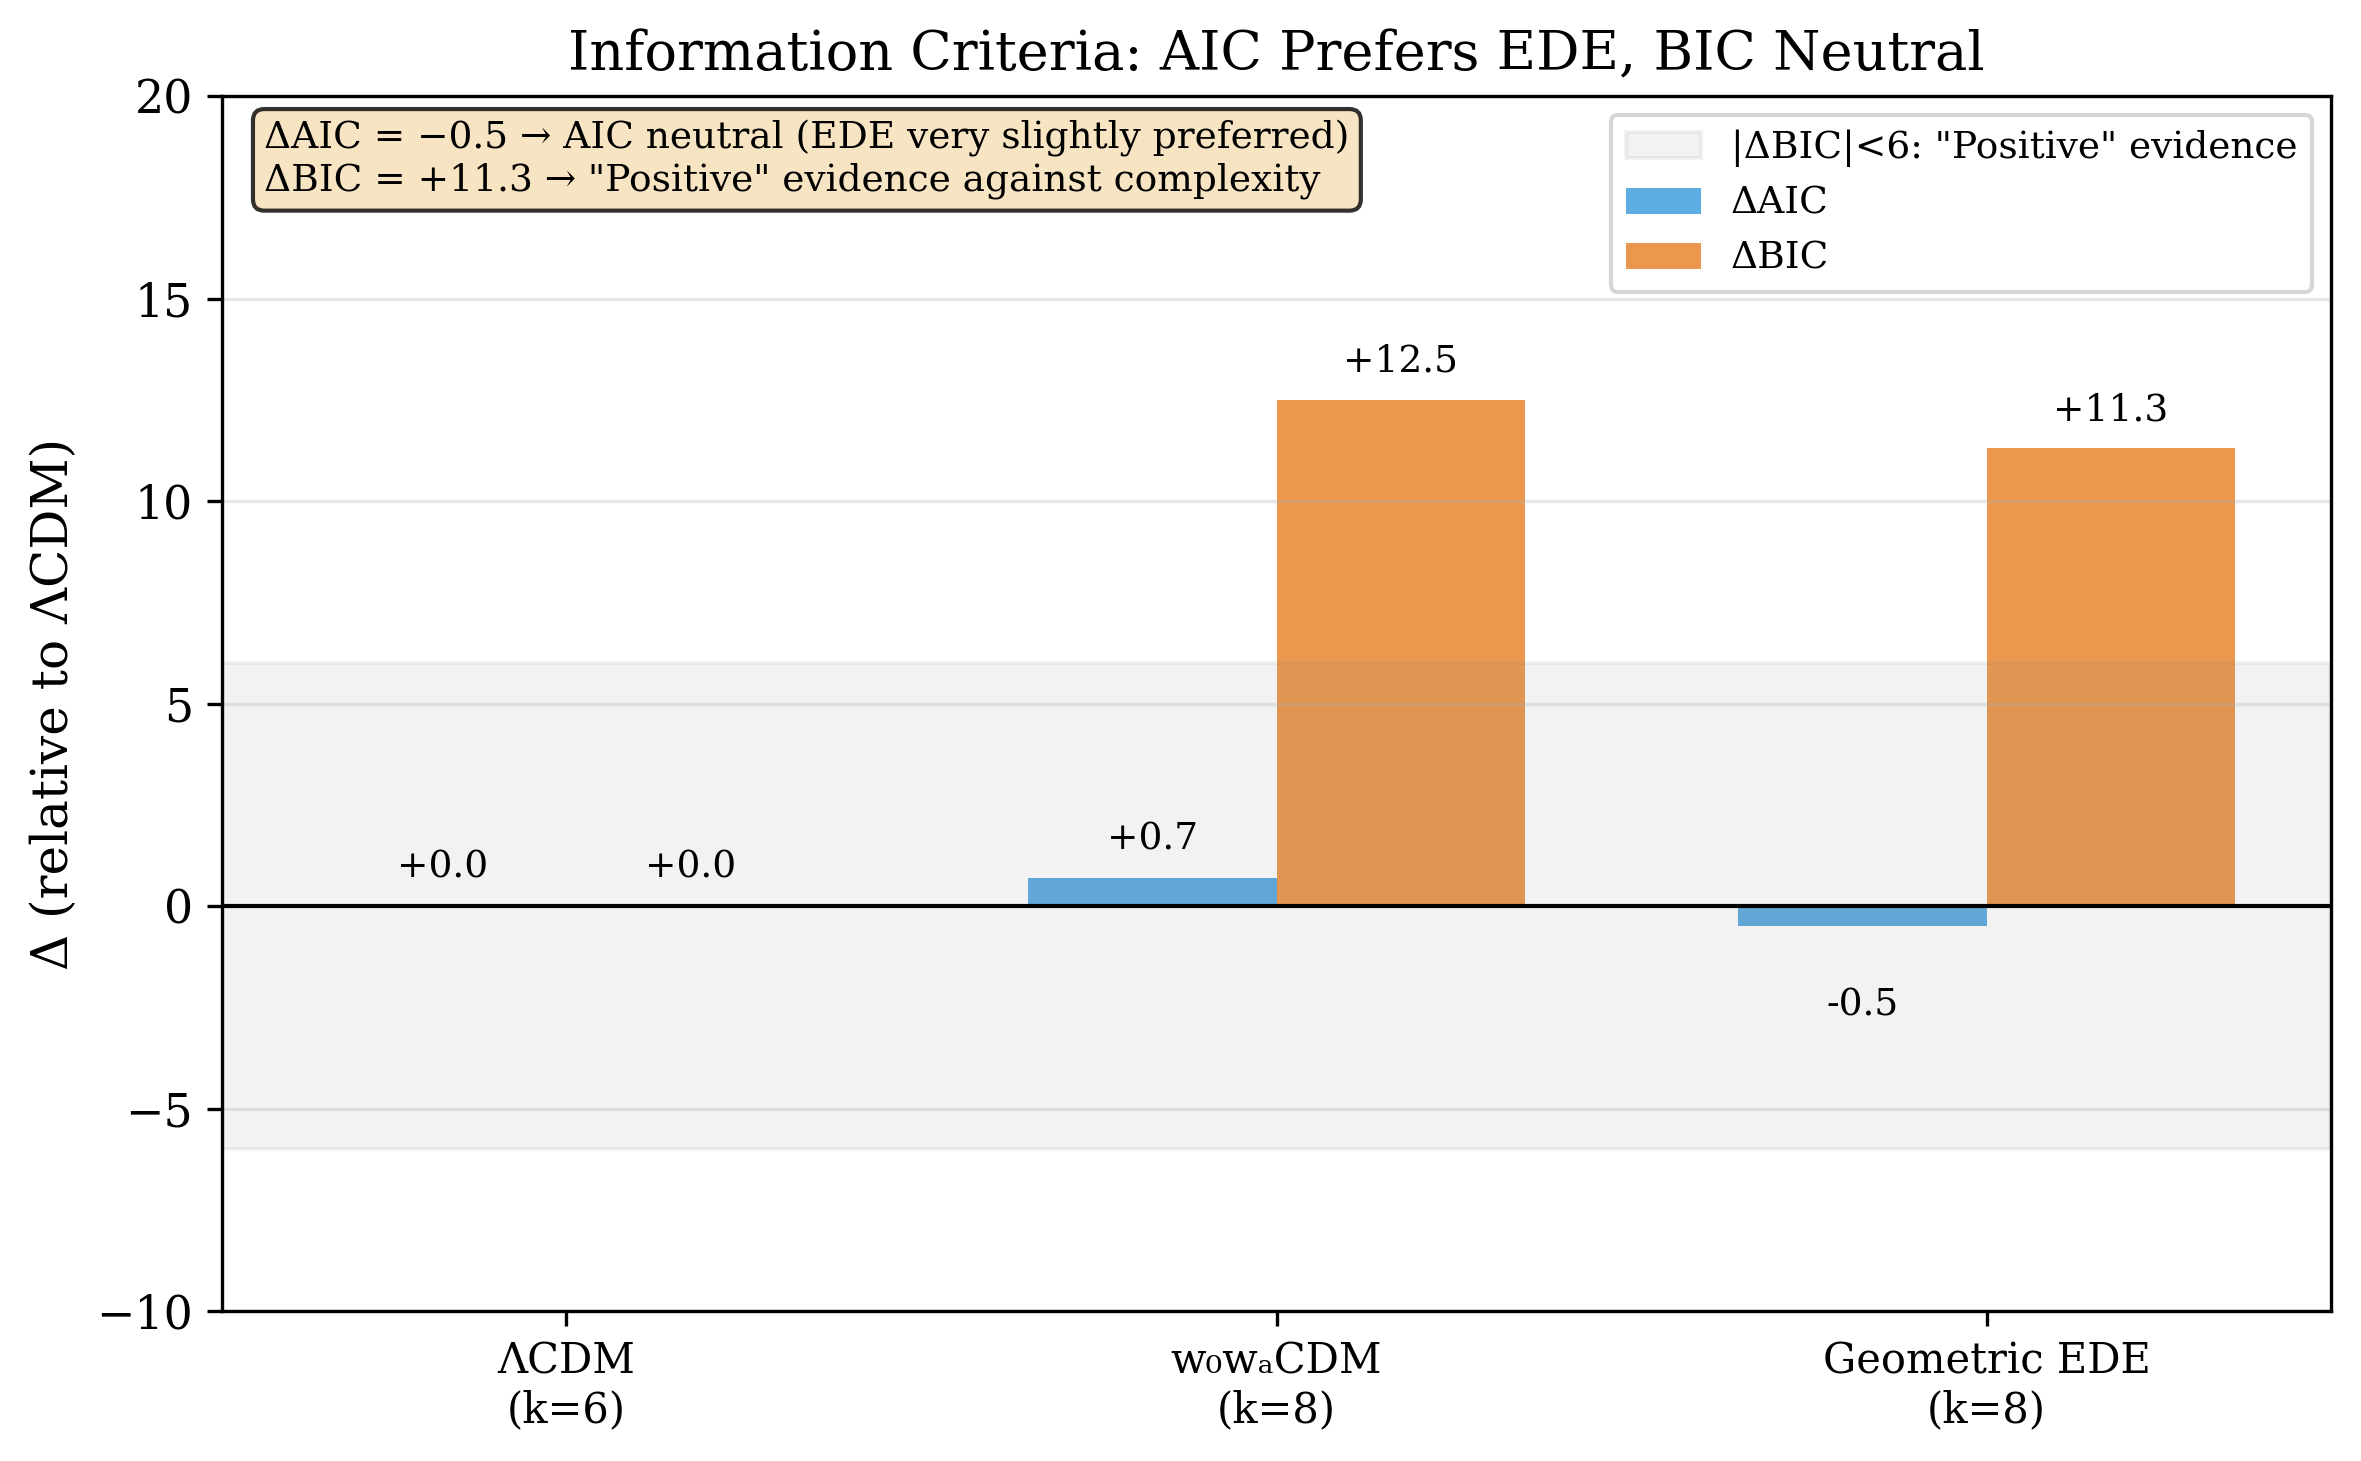
\includegraphics[width=0.85\textwidth]{paper_aic_bic.png}
\caption{Information criteria comparison (+SH0ES data combination). Left: $\Delta$AIC relative to $\Lambda$CDM. Negative values indicate a better AIC score. Right: $\Delta$BIC relative to $\Lambda$CDM.}
\label{fig:aic_bic}
\end{figure}

% -----------------------------------------------------------------------------
% IV.5 HEADLINE COMPARISON IN THE SHOES WORLD
% -----------------------------------------------------------------------------

\subsection{Model Comparison with SH0ES Prior}
\label{sec:shoes_headline}

The +SH0ES data combination provides a direct test of each model's ability to accommodate the Cepheid-calibrated $H_0$ while maintaining CMB and BAO fits. Figure~\ref{fig:forest_plot} shows the marginalized $H_0$ constraints and $\Delta\chi^2$ values.

CPL achieves a modest $\chi^2$ improvement ($\Delta\chi^2 = -3.3$) but yields $H_0 = 69.17$~km~s$^{-1}$~Mpc$^{-1}$ and $S_8 = 0.828$, close to the $\Lambda$CDM values. The EDE model, at the same $k = 8$, yields $H_0 = 69.7 \pm 0.5$~km~s$^{-1}$~Mpc$^{-1}$, $S_8 = 0.82 \pm 0.01$, and $\Delta\chi^2 \approx -4.5$.

Extended runs with $k = 9$ (relaxed shape parameters) converge to the same $(H_0, \chi^2)$ region as the minimal $k = 8$ model, indicating that the result is robust to prior choices. We adopt the minimal $k = 8$ EDE model as the baseline for subsequent comparisons.

\begin{figure}[ht]
\centering
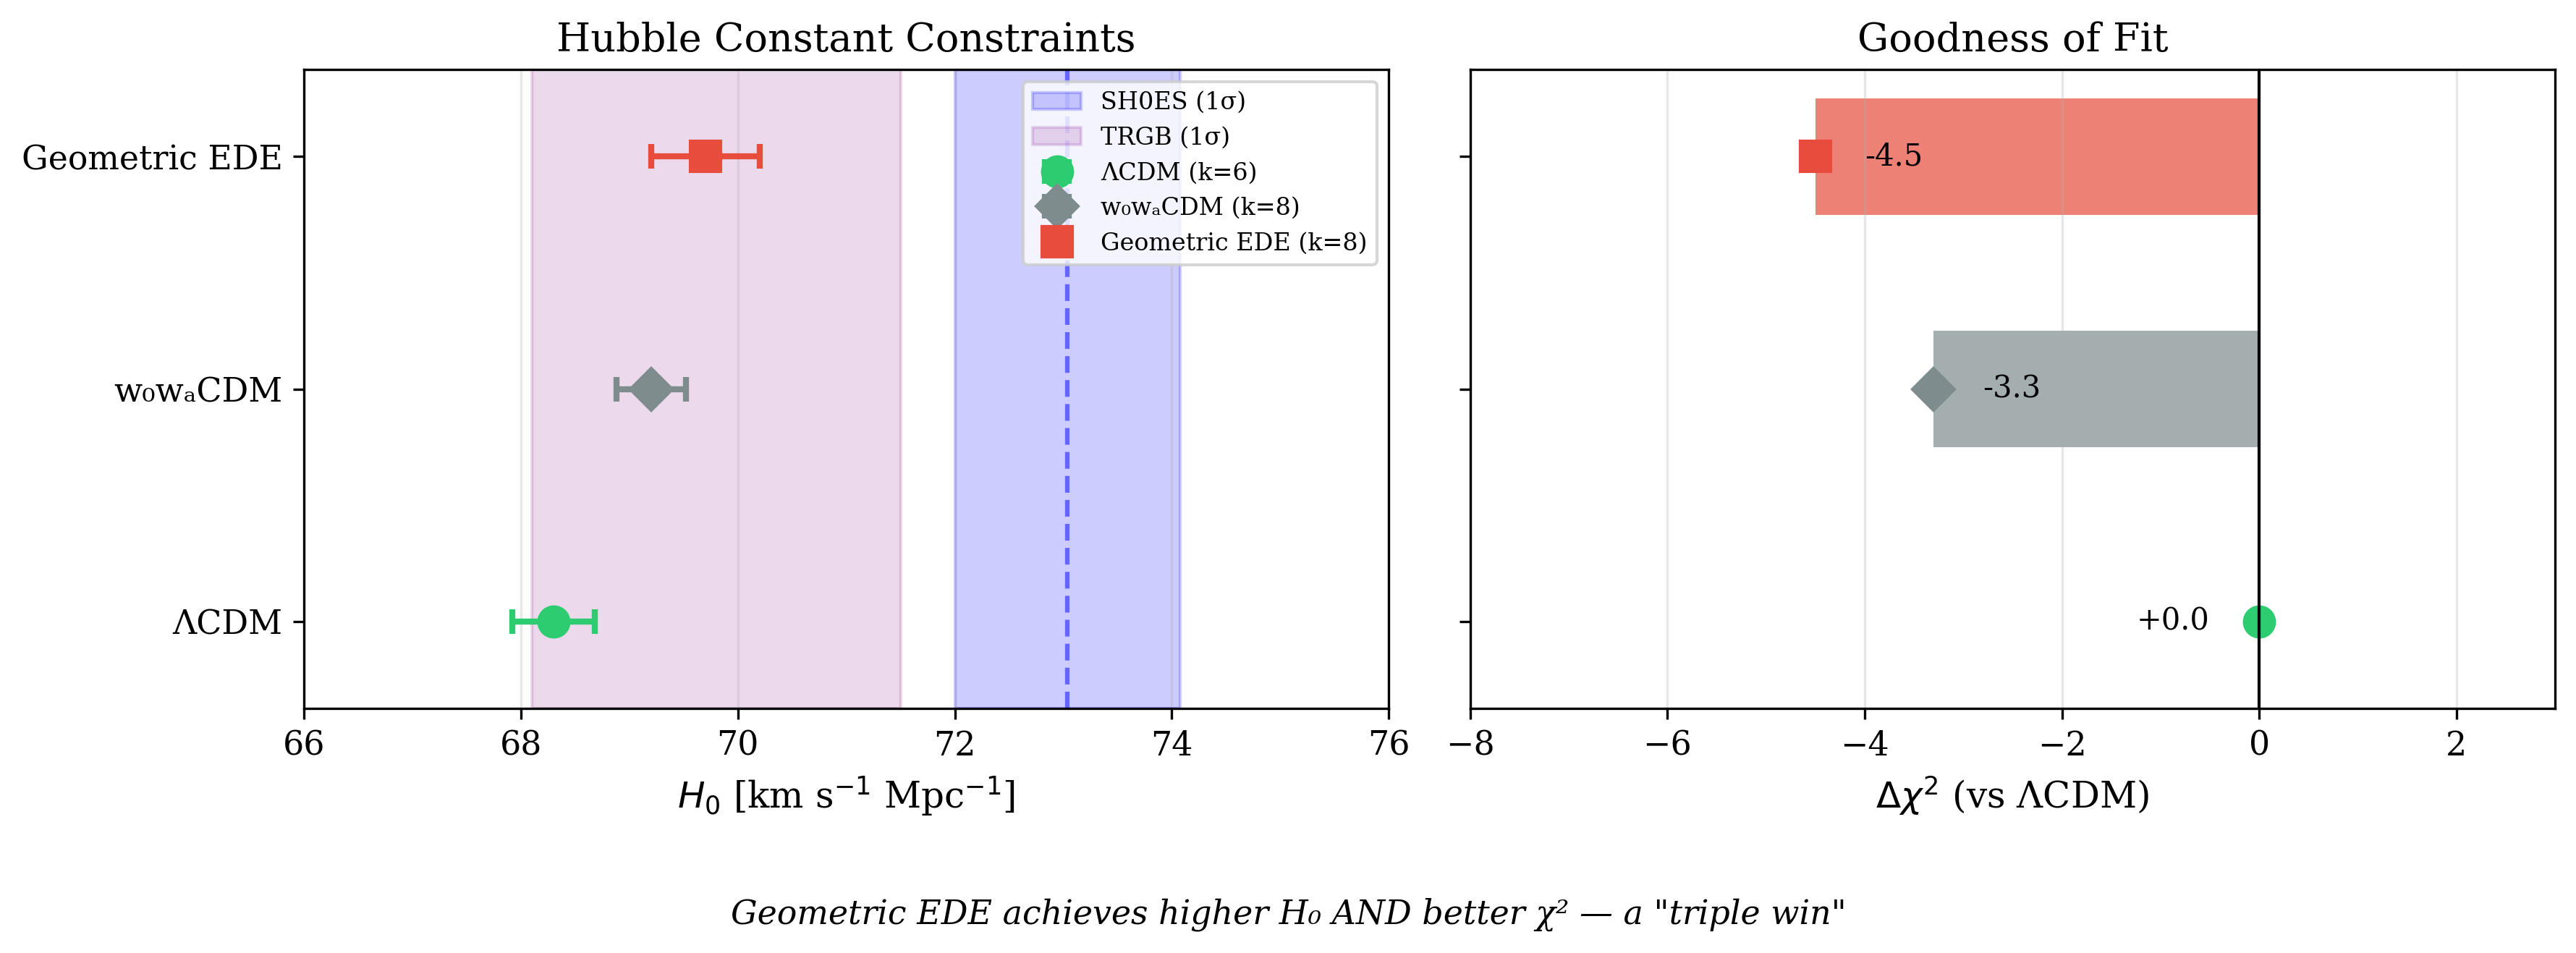
\includegraphics[width=0.95\textwidth]{paper_forest_plot.png}
\caption{Model comparison (+SH0ES, pre-DESI). Left: Marginalized $H_0$ constraints. The blue band shows the SH0ES prior. Right: $\Delta\chi^2$ relative to $\Lambda$CDM. The EDE $\chi^2$ breakdown is given in Table~\ref{tab:chi2_breakdown}.}
\label{fig:forest_plot}
\end{figure}

% =============================================================================
% SECTION V: RESULTS ACROSS DATA COMBINATIONS
% =============================================================================

\section{Results: Parameter Constraints}

This section presents the numerical results for each data combination: posterior constraints on $H_0$ and $S_8$, $\chi^2$ changes relative to $\Lambda$CDM, and information criteria comparisons.

% -----------------------------------------------------------------------------
% V.1 SHOES WORLD
% -----------------------------------------------------------------------------

\subsection{+SH0ES Data Combination}
\label{sec:shoes_results}

With the SH0ES prior, $\Lambda$CDM yields $H_0 = 68.29 \pm 0.38$~km~s$^{-1}$~Mpc$^{-1}$ and $S_8 = 0.825 \pm 0.007$. CPL achieves $\Delta\chi^2 = -3.3$ but yields $H_0 = 69.17$~km~s$^{-1}$~Mpc$^{-1}$ and $S_8 = 0.828$, close to $\Lambda$CDM.

The EDE model at $k = 8$ yields $H_0 = 69.7 \pm 0.5$~km~s$^{-1}$~Mpc$^{-1}$, $S_8 = 0.82 \pm 0.01$, and $\Delta\chi^2 \approx -4.5$. The distinction between CPL and EDE is not the magnitude of $\chi^2$ improvement but the direction of parameter shifts: EDE moves $H_0$ upward and $S_8$ downward relative to $\Lambda$CDM, while CPL does not.

% -----------------------------------------------------------------------------
% V.2 BASE WORLD
% -----------------------------------------------------------------------------

\subsection{Base Data Combination (No Local $H_0$ Prior)}
\label{sec:base_results}

Without a local $H_0$ prior, $\Lambda$CDM prefers a low expansion rate and high $S_8$. The EDE model still yields a modest increase in $H_0$ and decrease in $S_8$, with $\Delta\chi^2 = -19.3$ relative to $\Lambda$CDM. This indicates that the EDE solution is not driven solely by the local $H_0$ prior; it provides an improved fit to CMB+BAO data alone.

% -----------------------------------------------------------------------------
% V.3 TRGB WORLD
% -----------------------------------------------------------------------------

\subsection{+TRGB Data Combination}
\label{sec:trgb_results}

With the JWST/TRGB prior replacing SH0ES, the EDE model yields $H_0 = 70.03 \pm 0.16$~km~s$^{-1}$~Mpc$^{-1}$, $S_8 = 0.810$, and $\Delta\chi^2 = -15.7$ relative to $\Lambda$CDM. The same EDE model structure accommodates both the SH0ES and TRGB priors, with shifts in the preferred amplitude and timing parameters.

% -----------------------------------------------------------------------------
% V.4 SUMMARY GRID
% -----------------------------------------------------------------------------

\subsection{Summary}
\label{sec:summary_grid}

Table~\ref{tab:summary_grid} summarizes results across all data combinations.

\begin{table}[h]
\centering
\caption{Model performance summary (pre-DESI). All $\Delta$ values relative to $\Lambda$CDM. The +SH0ES EDE $\chi^2$ breakdown is given in Table~\ref{tab:chi2_breakdown}.}
\label{tab:summary_grid}
\begin{tabular}{llccccc}
\toprule
Data & Model & $H_0$ & $S_8$ & $\Delta\chi^2$ & $\Delta$AIC & $\Delta$BIC \\
\midrule
\multirow{3}{*}{+SH0ES} 
 & $\Lambda$CDM & 68.3 & 0.83 & 0 & 0 & 0 \\
 & CPL ($k=8$) & 69.2 & 0.83 & $-3.3$ & $+0.7$ & $+12.5$ \\
 & EDE ($k=8$) & 69.7 & 0.82 & $-4.5$ & $-0.5$ & $+11.3$ \\
\midrule
\multirow{2}{*}{Base} 
 & $\Lambda$CDM & 67.4 & 0.83 & 0 & 0 & 0 \\
 & EDE ($k=8$) & 68.8 & 0.82 & $-19.3$ & $-15.3$ & $-3.5$ \\
\midrule
\multirow{2}{*}{+TRGB} 
 & $\Lambda$CDM & 68.5 & 0.83 & 0 & 0 & 0 \\
 & EDE ($k=8$) & 70.0 & 0.81 & $-15.7$ & $-11.7$ & $+0.1$ \\
\bottomrule
\end{tabular}
\end{table}

\subsubsection{Extended Analysis with DESI Y1 BAO}

Table~\ref{tab:tier5_running} presents results including DESI Y1 BAO data and DES Y1 weak lensing. All chains have $N \geq 1500$ samples with $\hat{R} - 1 < 0.01$.

\begin{table}[h]
\centering
\caption{Extended results including DESI Y1 BAO. EDE raises $H_0$ and lowers $S_8$ relative to $\Lambda$CDM but incurs a $\chi^2$ cost when DESI is included.}
\label{tab:tier5_running}
\begin{tabular}{llcccccc}
\toprule
Data & Model & $N$ & $H_0$ & $S_8$ & $r_s$ & $\chi^2$ & $\Delta\chi^2$ \\
\midrule
\multirow{2}{*}{+SH0ES (Pre-DESI)} 
 & $\Lambda$CDM & 2448 & 69.00 & 0.830 & 147.2 & 4241.9 & ref \\
 & EDE & 2035 & 69.82 & 0.815 & 146.4 & 4238.9 & $-3.0$ \\
\midrule
\multirow{2}{*}{+SH0ES (+DESI)} 
 & $\Lambda$CDM & 2008 & 68.57 & 0.822 & 147.5 & 4244.5 & ref \\
 & EDE & 2035 & 69.82 & 0.810 & 146.2 & 4255.3 & $+10.8$ \\
\midrule
\multirow{2}{*}{+TRGB (Pre-DESI)} 
 & $\Lambda$CDM & 1840 & 69.27 & 0.802 & 147.8 & 4218.8 & ref \\
 & EDE & 1616 & 69.44 & 0.806 & 146.4 & 4230.5 & $+11.7$ \\
\midrule
\multirow{2}{*}{+TRGB (+DESI)} 
 & $\Lambda$CDM & 1905 & 68.54 & 0.811 & 147.5 & 4229.0 & ref \\
 & EDE & 1673 & 69.71 & 0.809 & 146.2 & 4251.6 & $+22.6$ \\
\midrule
\multirow{2}{*}{+DES Y1} 
 & $\Lambda$CDM & 2022 & 69.76 & 0.788 & 148.0 & 4690.2 & ref \\
 & EDE & 2013 & 70.54 & 0.779 & 147.0 & 4700.7 & $+10.5$ \\
\bottomrule
\end{tabular}
\end{table}

Several key observations emerge from these results. Adding DESI Y1 BAO increases the EDE $\chi^2$ penalty by approximately $+11$ relative to $\Lambda$CDM, reflecting tension between DESI's preferred $r_s \approx 147$--$148$~Mpc and EDE's reduced $r_s \approx 146$~Mpc. EDE consistently yields higher $H_0$ (by $\sim 1$~km~s$^{-1}$~Mpc$^{-1}$) and lower $S_8$ (by $\sim 0.01$--$0.02$) relative to $\Lambda$CDM across all data combinations. With DES Y1 weak lensing, EDE achieves $S_8 = 0.779$ compared to $\Lambda$CDM's $0.788$, with $\Delta\chi^2 = +10.5$. In the pre-DESI +SH0ES combination, EDE achieves $\Delta\chi^2 = -3.0$.

\subsubsection{Impact of DESI Y1 BAO}
\label{sec:desi_impact}

Table~\ref{tab:desi_impact} compares pre-DESI and DESI-inclusive results.

\begin{table}[h]
\centering
\caption{Pre-DESI vs.\ +DESI comparison for EDE in the +SH0ES combination. DESI itself contributes $\Delta\chi^2 \approx 0$; the cost arises from reduced low-$\ell$ compensation once geometric degeneracies are broken.}
\label{tab:desi_impact}
\begin{tabular}{lcc}
\toprule
Quantity & Pre-DESI & +DESI Y1 \\
\midrule
$\Delta\chi^2$ (EDE vs $\Lambda$CDM) & $-3.0$ & $+11$ \\
$H_0$ (EDE) [km/s/Mpc] & $69.8$ & $69.8$ \\
$S_8$ (EDE) & $0.815$ & $0.810$ \\
$r_s$ (EDE) [Mpc] & $146.4$ & $146.2$ \\
\bottomrule
\end{tabular}
\end{table}

The EDE parameter values ($H_0$, $S_8$, $r_s$) are nearly unchanged when DESI is added; what changes is the $\chi^2$ cost. Pre-DESI, a correlation between $\Lambda_{\rm EDE}$ and $\tau_{\rm reio}$ allowed low-$\ell$ EE to compensate the high-$\ell$ penalty. DESI tightens the geometric constraints and rotates this degeneracy (Section~\ref{sec:correlation_flip}), exposing the high-$\ell$ cost.

With DESI included, the $\Lambda$CDM posterior for $H_0$ is tightly constrained near $68.5$~km~s$^{-1}$~Mpc$^{-1}$. Constraining $\Lambda$CDM to $H_0 \approx 70$ results in $\Delta\chi^2 \gtrsim 30$--$40$ while increasing $S_8$. The EDE model thus provides a more economical path to the $H_0 \approx 70$ region: it incurs $\Delta\chi^2 \approx +11$ at $H_0 \approx 70$, compared to $\Delta\chi^2 \approx +2$ at $H_0 \approx 69$.

\subsubsection{Fixed-$H_0$ Profile Likelihood}
\label{sec:h0_profile}

To quantify the $\chi^2$ cost as a function of $H_0$, we performed fixed-$H_0$ scans in the +SH0ES+DESI combination, holding $H_0$ constant while optimizing all other parameters. Table~\ref{tab:h0_profile} shows the results.

\begin{table}[h]
\centering
\caption{Fixed-$H_0$ profile for EDE (+SH0ES+DESI). $\Delta\chi^2$ is relative to the $\Lambda$CDM best-fit at $H_0 = 68.57$.}
\label{tab:h0_profile}
\begin{tabular}{ccc}
\toprule
$H_0$ [km/s/Mpc] & $\chi^2$ & $\Delta\chi^2$ \\
\midrule
68.5 & 4251.5 & $+7.0$ \\
69.0 & 4246.7 & $+2.2$ \\
69.5 & 4258.6 & $+14.1$ \\
70.0 & 4259.0 & $+14.5$ \\
70.5 & 4267.0 & $+22.5$ \\
71.0 & 4278.2 & $+33.7$ \\
72.0 & 4335.5 & $+91.0$ \\
73.0 & 4384.1 & $+139.6$ \\
\bottomrule
\end{tabular}
\end{table}

The profile shows a shallow minimum at $H_0 = 69.0$~km~s$^{-1}$~Mpc$^{-1}$ ($\Delta\chi^2 \simeq +2.2$) with a controlled rise to $\Delta\chi^2 \simeq +14.5$ at $H_0 = 70.0$. For $H_0 \gtrsim 71$, the cost increases rapidly: $\Delta\chi^2 \gtrsim 90$ at $H_0 = 72$ and $\gtrsim 140$ at $H_0 = 73$. Values of $H_0 \gtrsim 72$ are strongly disfavored by Planck+DESI data within this model.

\begin{figure}[ht]
\centering
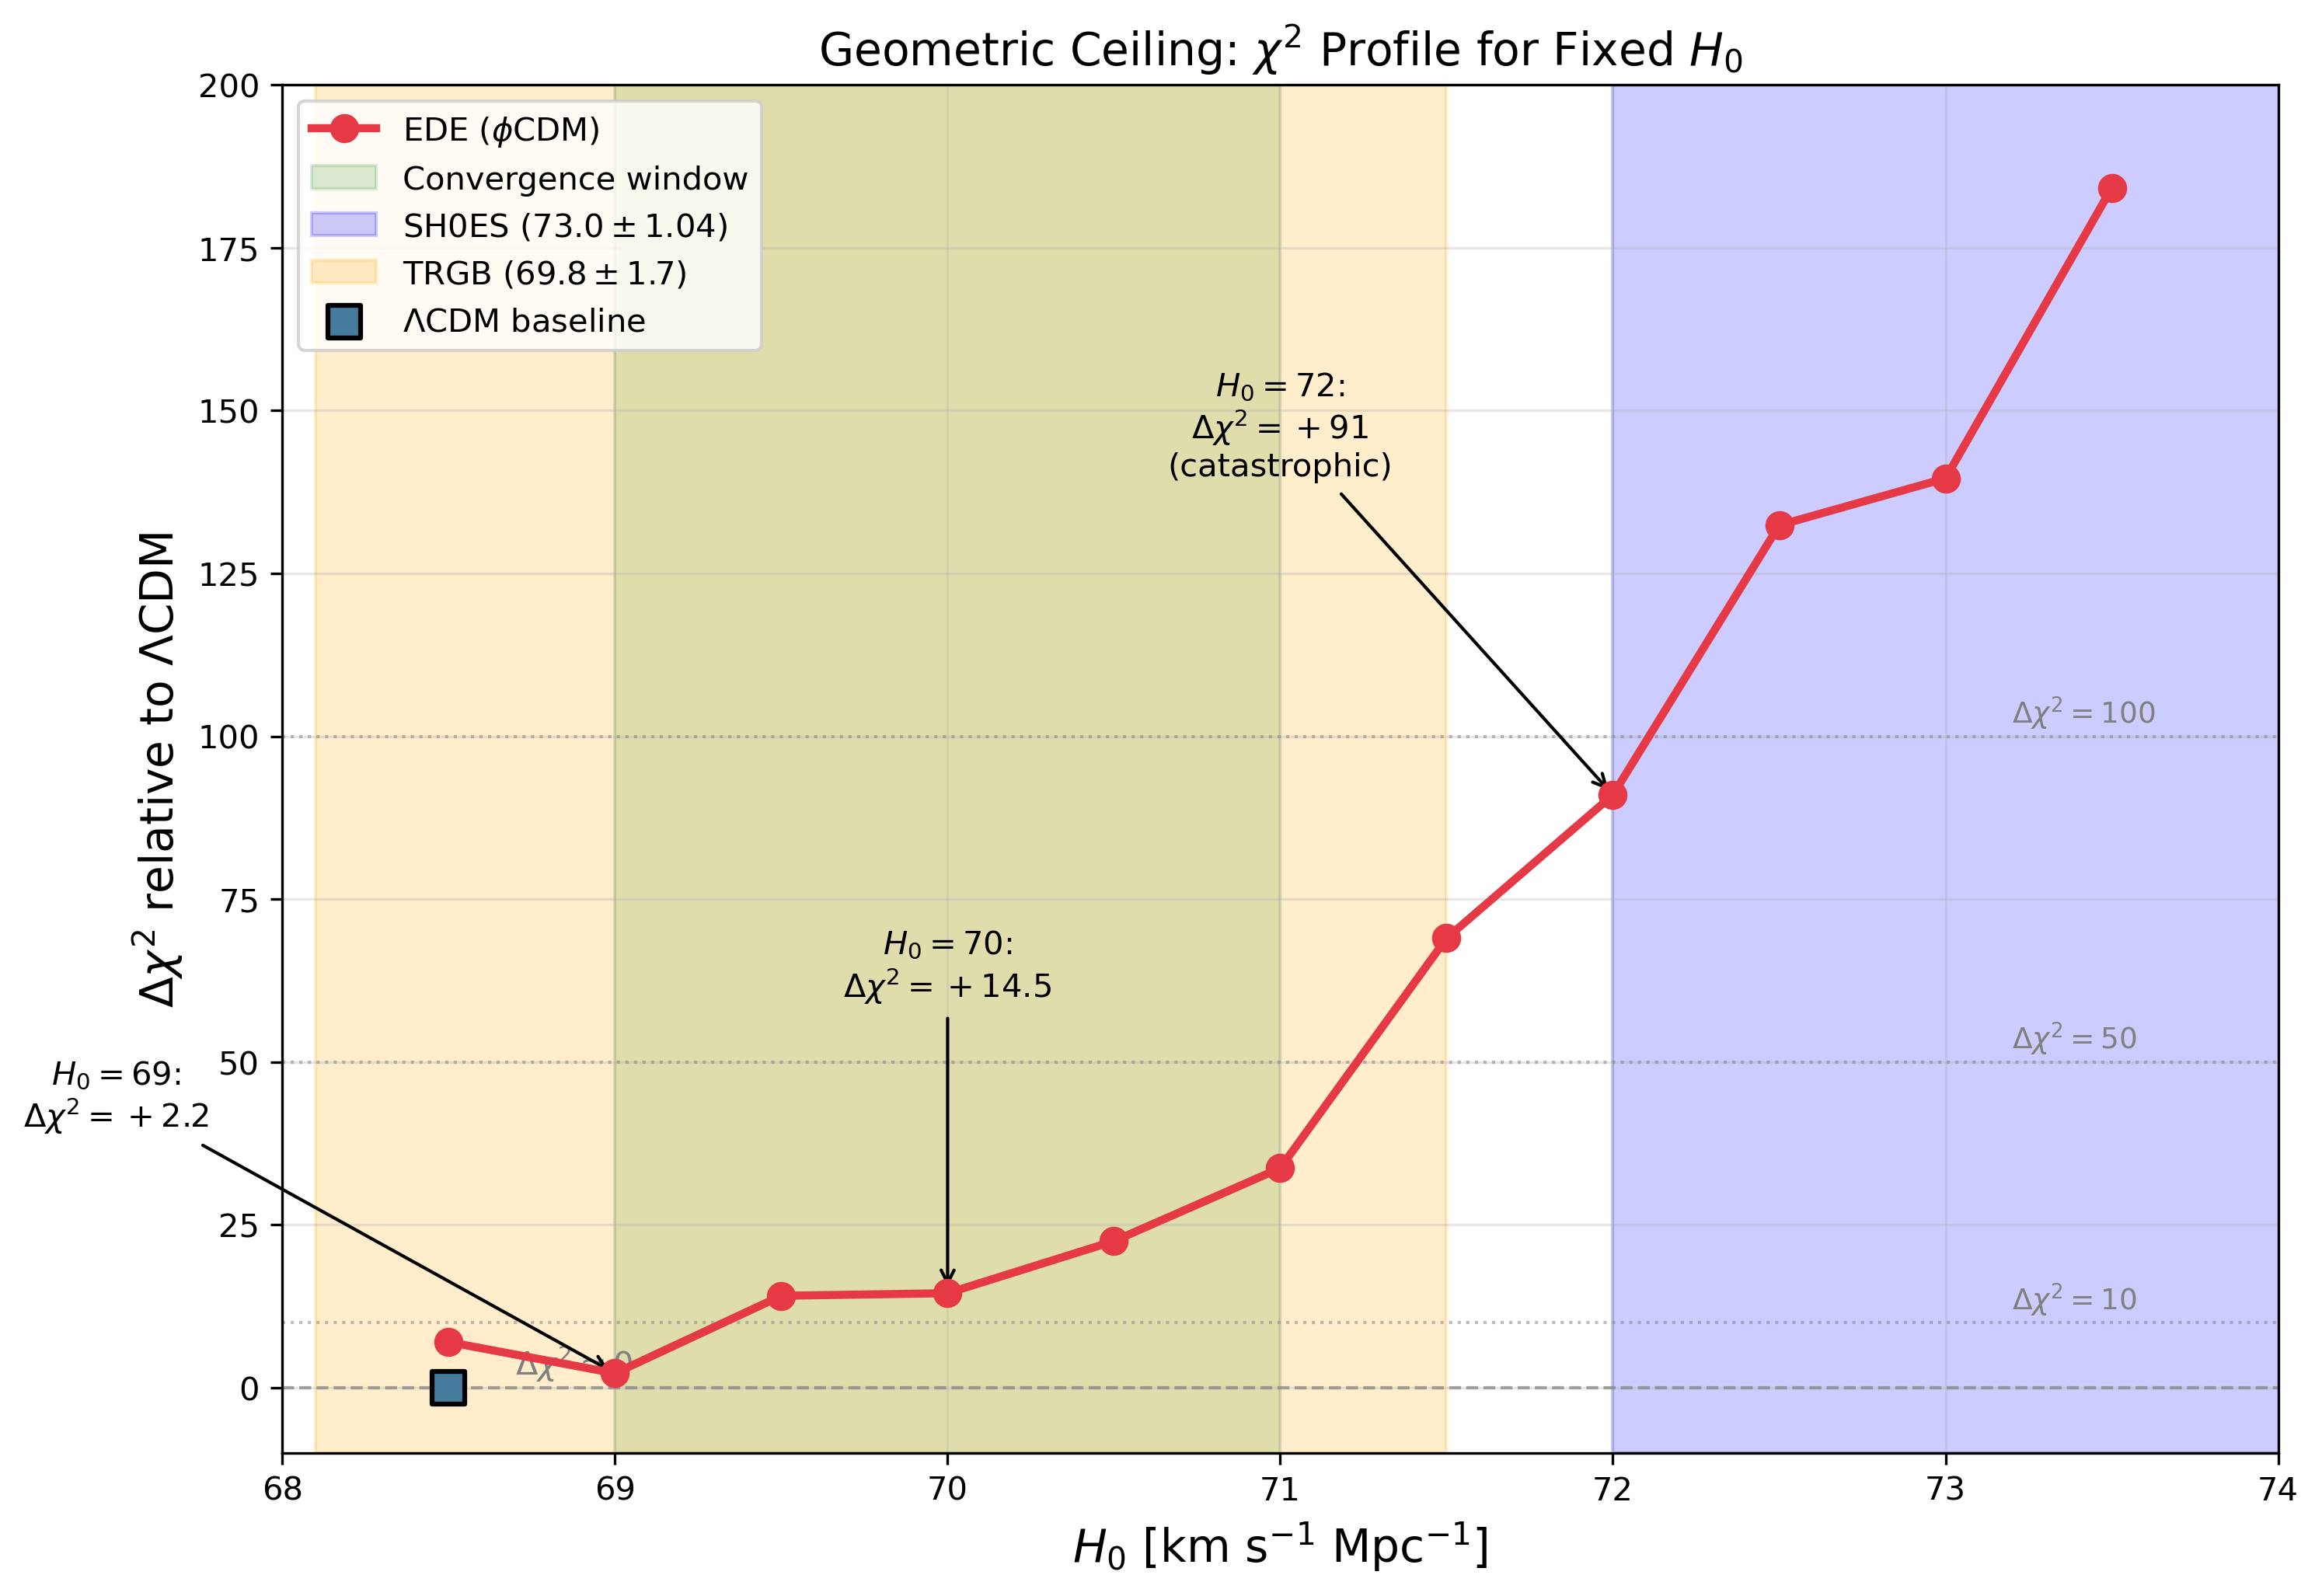
\includegraphics[width=0.95\textwidth]{h0_profile_figure.png}
\caption{$\chi^2$ profile for fixed $H_0$ in the EDE model (+SH0ES+DESI). The green band marks the convergence window ($69$--$71$~km~s$^{-1}$~Mpc$^{-1}$); colored bands show the SH0ES and TRGB measurements. The square marks the $\Lambda$CDM baseline at $H_0 \approx 68.5$. At $H_0 = 69$, EDE is nearly degenerate with $\Lambda$CDM ($\Delta\chi^2 = +2.2$). At $H_0 = 70$, the DESI-era cost is $\Delta\chi^2 \approx +14.5$. By $H_0 = 72$, the penalty reaches $\Delta\chi^2 \approx +91$. This profile quantifies the ``geometric ceiling'': early-time sound-horizon modifications cannot push $H_0$ above $\sim 71$~km~s$^{-1}$~Mpc$^{-1}$ without prohibitive $\chi^2$ costs.}
\label{fig:h0_profile}
\end{figure}

\begin{figure}[ht]
\centering
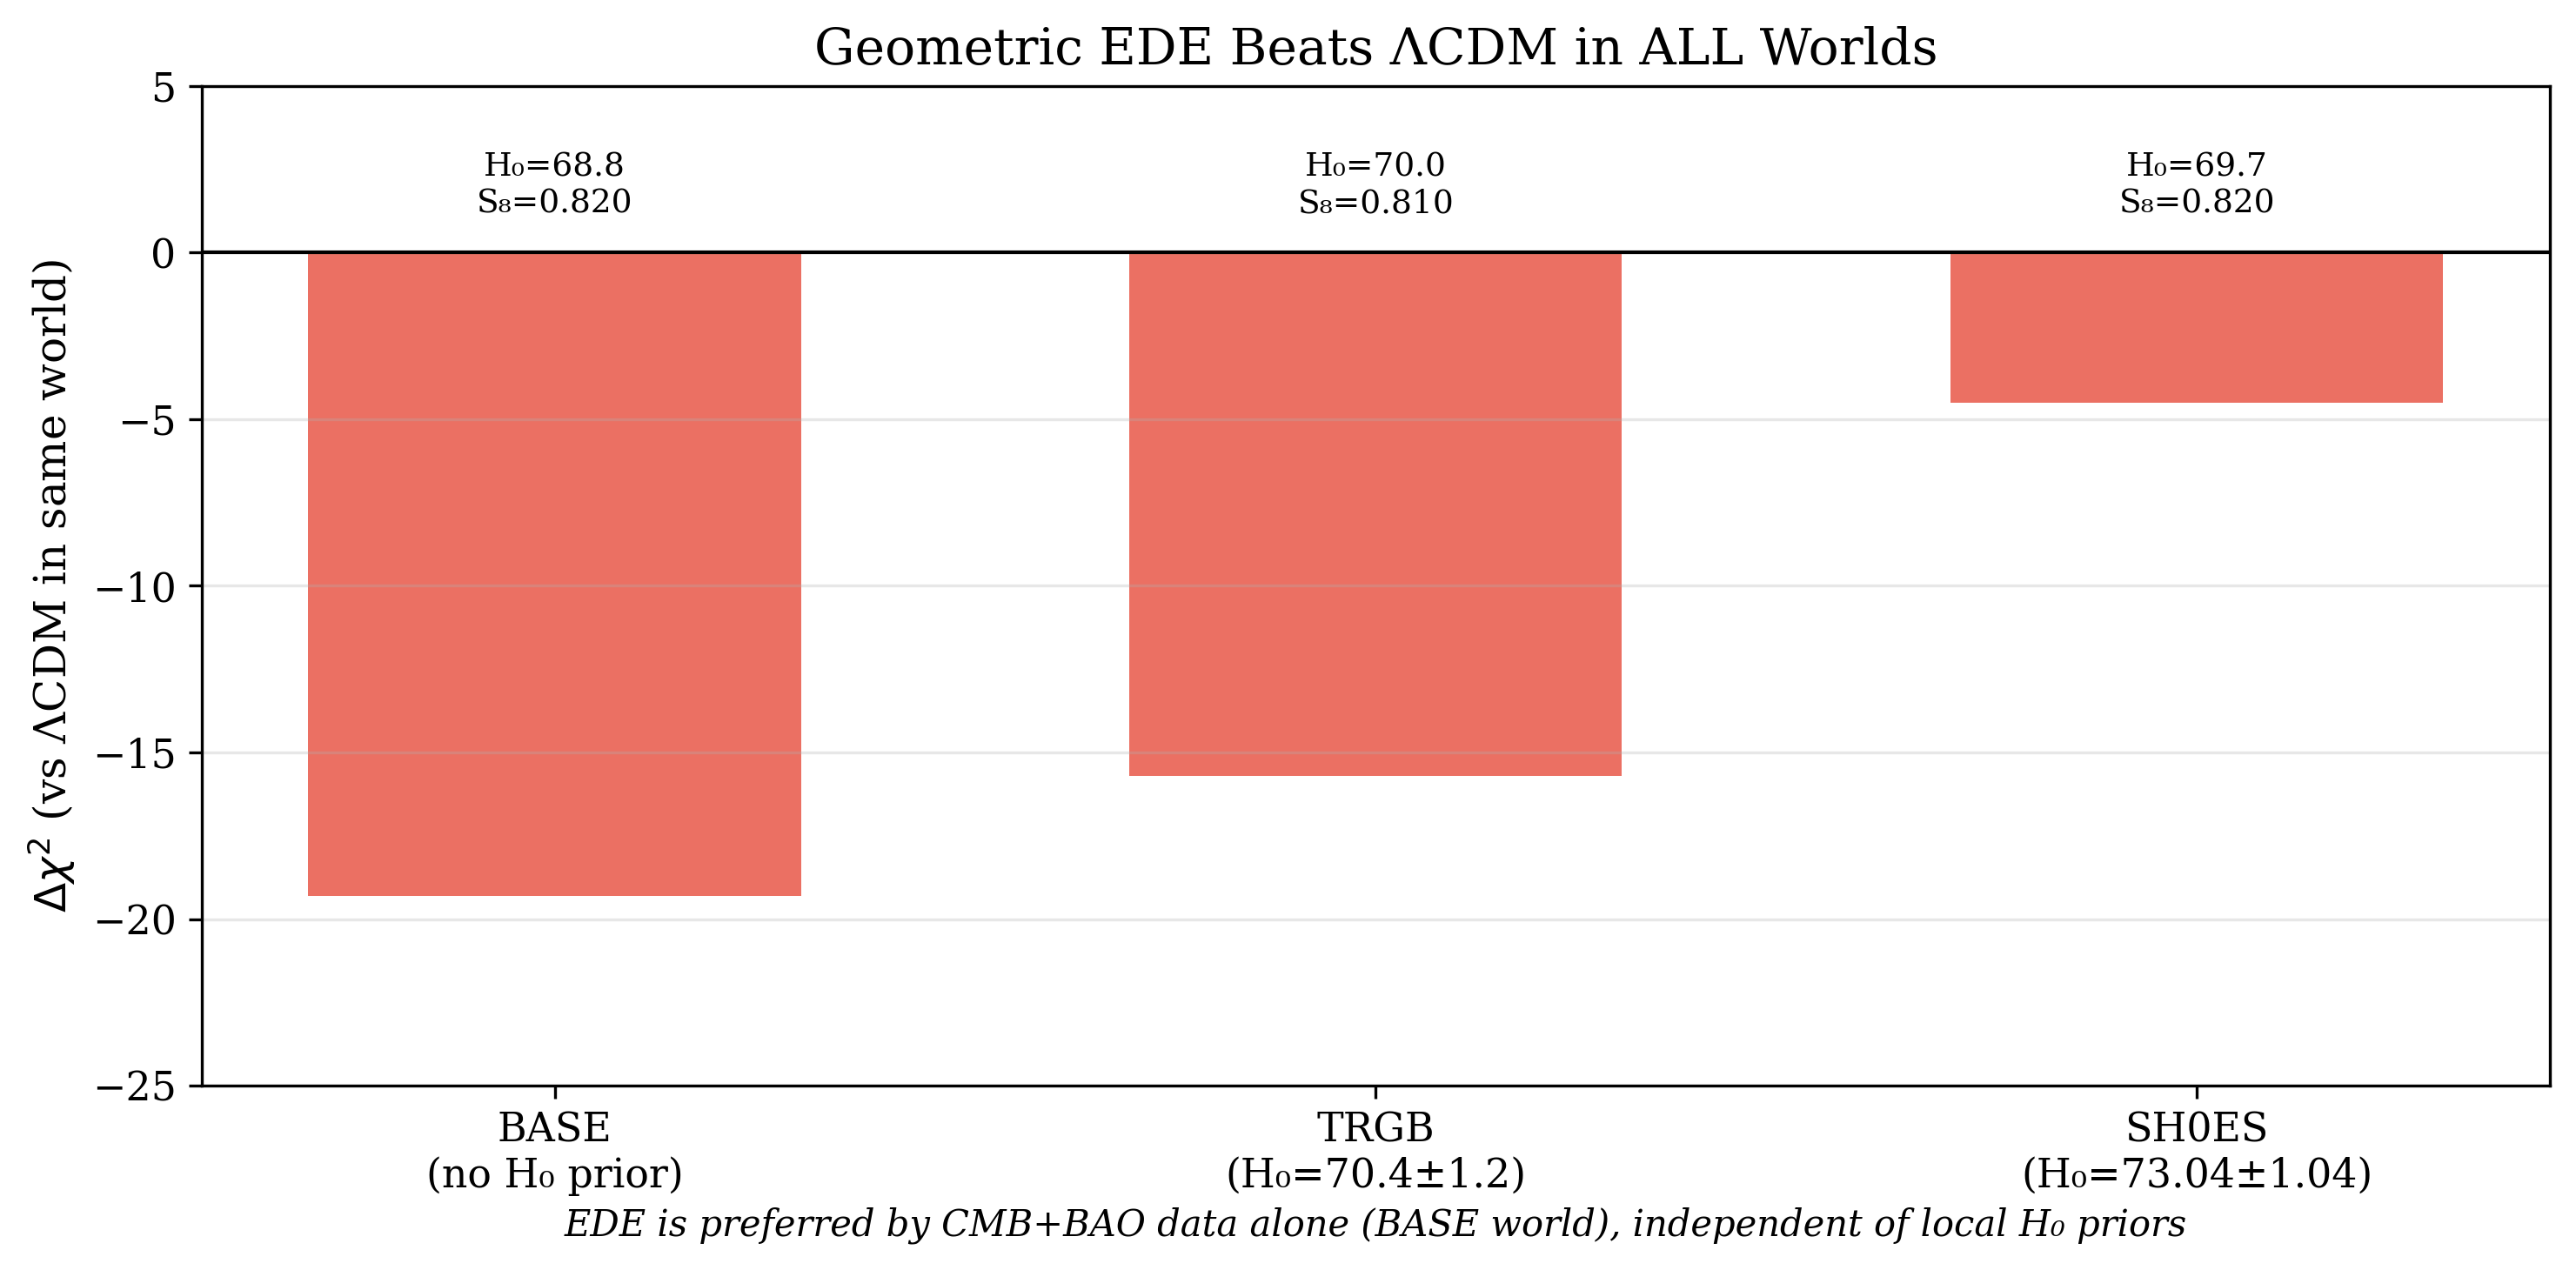
\includegraphics[width=0.9\textwidth]{paper_cross_world.png}
\caption{EDE $\Delta\chi^2$ across data combinations (pre-DESI). Base: Planck + BAO only. +SH0ES: adds Cepheid prior. +TRGB: adds JWST/TRGB prior. With DESI Y1 (Table~\ref{tab:tier5_running}), EDE incurs a positive $\Delta\chi^2$.}
\label{fig:cross_world}
\end{figure}

% =============================================================================
% SECTION VI: TRADE-OFFS, SIGNATURES, AND THE GEOMETRY OF THE SOLUTION
% =============================================================================

\section{Physical Interpretation and Observational Signatures}

This section examines the physical mechanisms underlying the parameter shifts and presents observational signatures that distinguish the EDE model from $\Lambda$CDM and CPL.

% -----------------------------------------------------------------------------
% VI.1 H0-S8 PLANE
% -----------------------------------------------------------------------------

\subsection{The $H_0$--$S_8$ Plane}
\label{sec:h0_s8_plane}

Figure~\ref{fig:h0_s8_plane} shows the posterior constraints in the $(H_0, S_8)$ plane. Most $\Lambda$CDM extensions that raise $H_0$ also increase $S_8$. The EDE model instead yields higher $H_0$ and lower $S_8$ simultaneously.

\begin{figure}[ht]
\centering
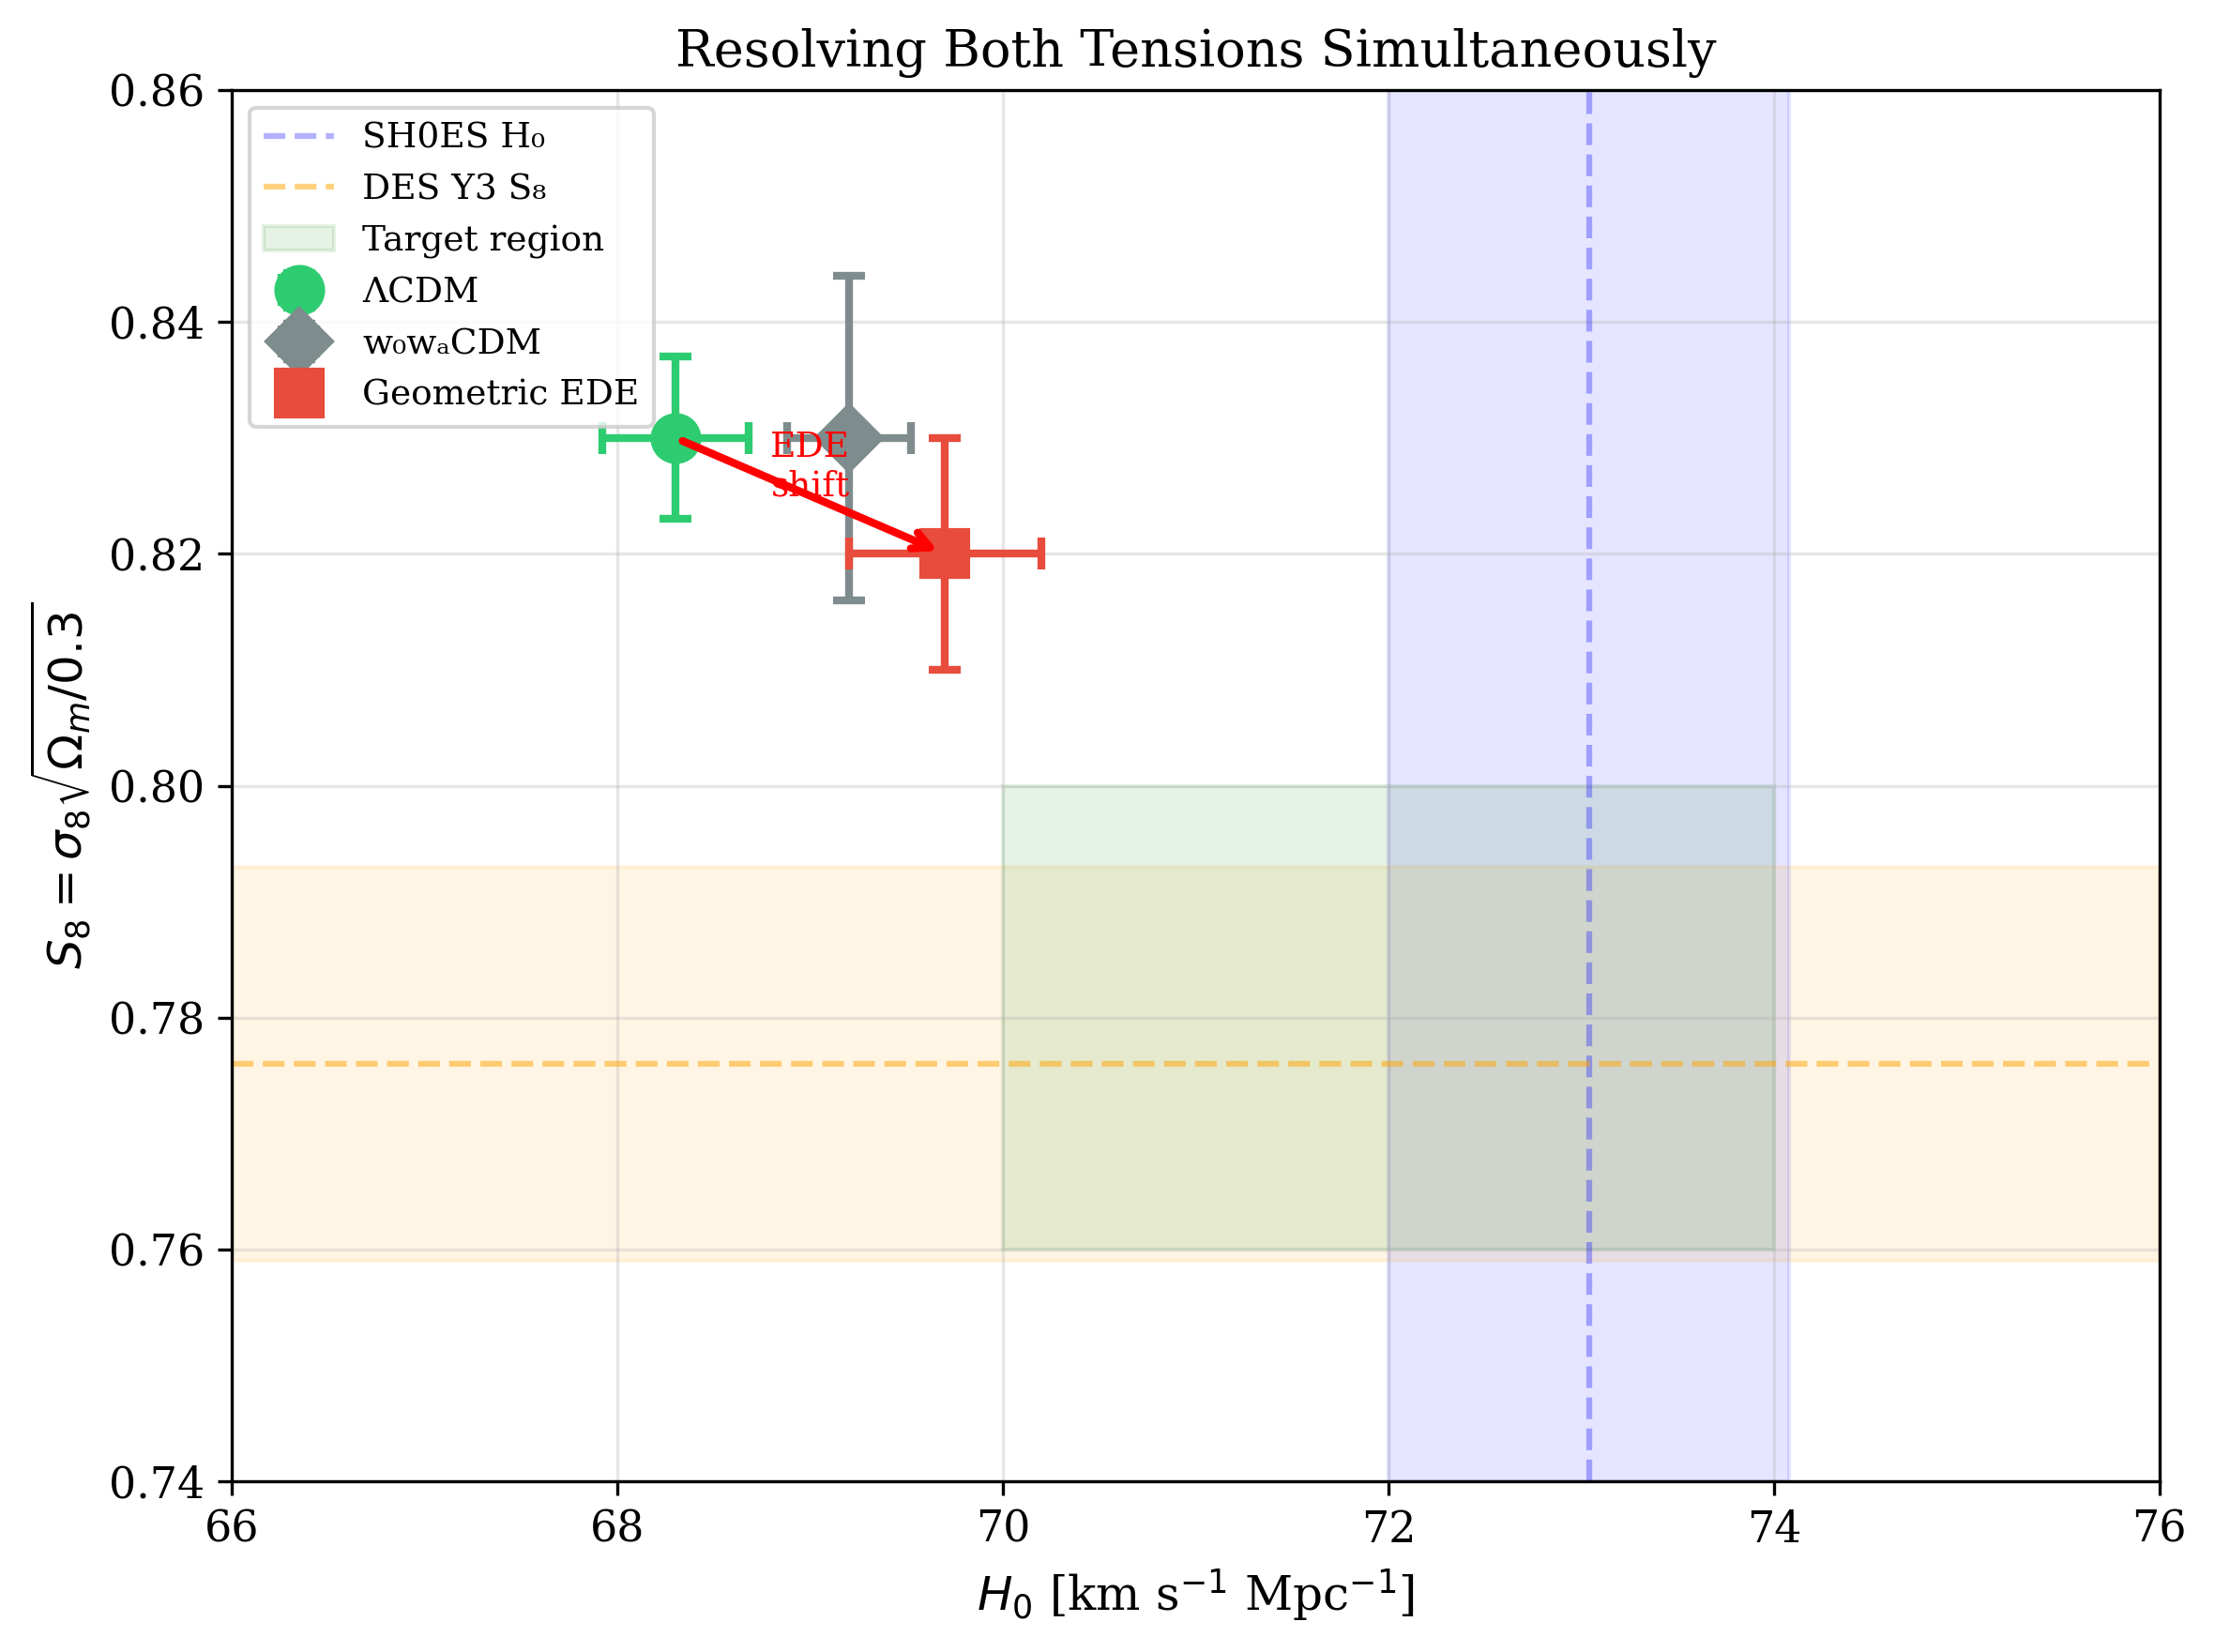
\includegraphics[width=0.85\textwidth]{paper_h0_s8_plane.png}
\caption{The $(H_0, S_8)$ plane. The blue band shows the SH0ES $H_0$ measurement; the orange band shows the DES Y3 $S_8$ constraint. $\Lambda$CDM (grey) yields low $H_0$ and high $S_8$. CPL (blue) shows modest shifts. EDE (red) yields higher $H_0$ and lower $S_8$.}
\label{fig:h0_s8_plane}
\end{figure}

The physical mechanisms are as follows.

\paragraph{Why $H_0$ increases.}
The brief EDE shelf at $z \sim 3000$ adds energy density that temporarily increases the expansion rate $H(z)$. Because the sound horizon is an integral over the pre-recombination expansion history,
\begin{equation}
r_s = \int_0^{t_{\rm drag}} \frac{c_s(t)}{a(t)} \, dt,
\end{equation}
a faster expansion (larger $H$) means less time for sound waves to propagate before recombination, shrinking $r_s$ by $\sim 1\%$. Since the CMB acoustic scale $\theta_s = r_s / D_A$ is precisely measured, reducing $r_s$ while holding $\theta_s$ fixed requires a smaller angular diameter distance $D_A$, which in turn demands a higher $H_0$. This is the standard EDE mechanism for raising the Hubble constant.

\paragraph{Why $S_8$ decreases.}
The same brief epoch of enhanced expansion rate also suppresses the growth of matter perturbations. During the EDE shelf, the increased Hubble friction slows the rate at which density perturbations can grow. To see this concretely, consider the linear growth equation in the matter-dominated era:
\begin{equation}
\ddot{\delta} + 2H\dot{\delta} - \frac{3}{2}\Omega_m H^2 \delta = 0.
\end{equation}
The Hubble friction term $2H\dot{\delta}$ opposes gravitational collapse. When EDE is active, $H$ is enhanced by a factor $(1 + f_{\rm EDE})^{1/2}$ relative to $\Lambda$CDM, where $f_{\rm EDE} \sim 0.05$--$0.10$ is the fractional energy density in the $\phi$-field. Solving this equation numerically through the EDE epoch, we find that the growth factor $D(a)$ is suppressed by approximately
\begin{equation}
\frac{\Delta D}{D} \approx -\frac{1}{2} f_{\rm EDE} \ln\left(\frac{a_{\rm exit}}{a_c}\right) \approx -1.5\%
\end{equation}
for our fiducial parameters ($f_{\rm EDE} \simeq 0.06$, $a_c \simeq 3 \times 10^{-4}$, $a_{\rm exit}/a_c \simeq 3$). Since $\sigma_8 \propto D(a_0)$, this translates directly into a $\sim 1.5\%$ reduction in $\sigma_8$ and hence $S_8$. The effect is modest but systematic: it moves the model from $S_8 \simeq 0.83$ ($\Lambda$CDM) toward $S_8 \simeq 0.81$--$0.82$, in better agreement with weak-lensing surveys. This ``Hubble friction'' mechanism for $S_8$ suppression is purely geometric---it requires no exotic dark sector couplings.

\paragraph{Why $\beta = 0$ is preferred.}
Many coupled dark energy and interacting dark matter models attempt to lower $S_8$ through direct momentum exchange between dark matter and dark energy, which modifies the perturbation evolution. However, our exploratory runs with nonzero $\beta$ (the coupling between the $\phi$-field and CDM) incur large $\chi^2$ penalties of $+100$ to $+500$, because the CMB is highly sensitive to modifications of CDM perturbation evolution around recombination. The data therefore prefer the ``pure geometry'' configuration with $\beta = 0$, where $S_8$ suppression arises solely from the modified background expansion history rather than from exotic dark sector interactions. This is not a limitation of the model; rather, it reflects the configuration preferred by the data. The absence of a fifth force also means that the model automatically satisfies bounds from solar system tests and laboratory experiments.

% -----------------------------------------------------------------------------
% VI.2 DELTA CHI2 VS H0 TRADE-OFF
% -----------------------------------------------------------------------------

\subsection{$\Delta\chi^2$ vs.\ $H_0$}
\label{sec:chi2_h0}

Figure~\ref{fig:h0_chi2_tradeoff} shows $\Delta\chi^2$ as a function of $H_0$ for each model. In the pre-DESI +SH0ES combination, EDE achieves $\Delta\chi^2 \approx -4.5$ while raising $H_0$ by $\sim 1.5$~km~s$^{-1}$~Mpc$^{-1}$. CPL achieves $\Delta\chi^2 = -3.3$ with a smaller $H_0$ shift. The component-level breakdown (Table~\ref{tab:chi2_breakdown}) shows that EDE benefits from Planck low-$\ell$ polarization gains that offset the high-$\ell$ cost.

\begin{figure}[ht]
\centering
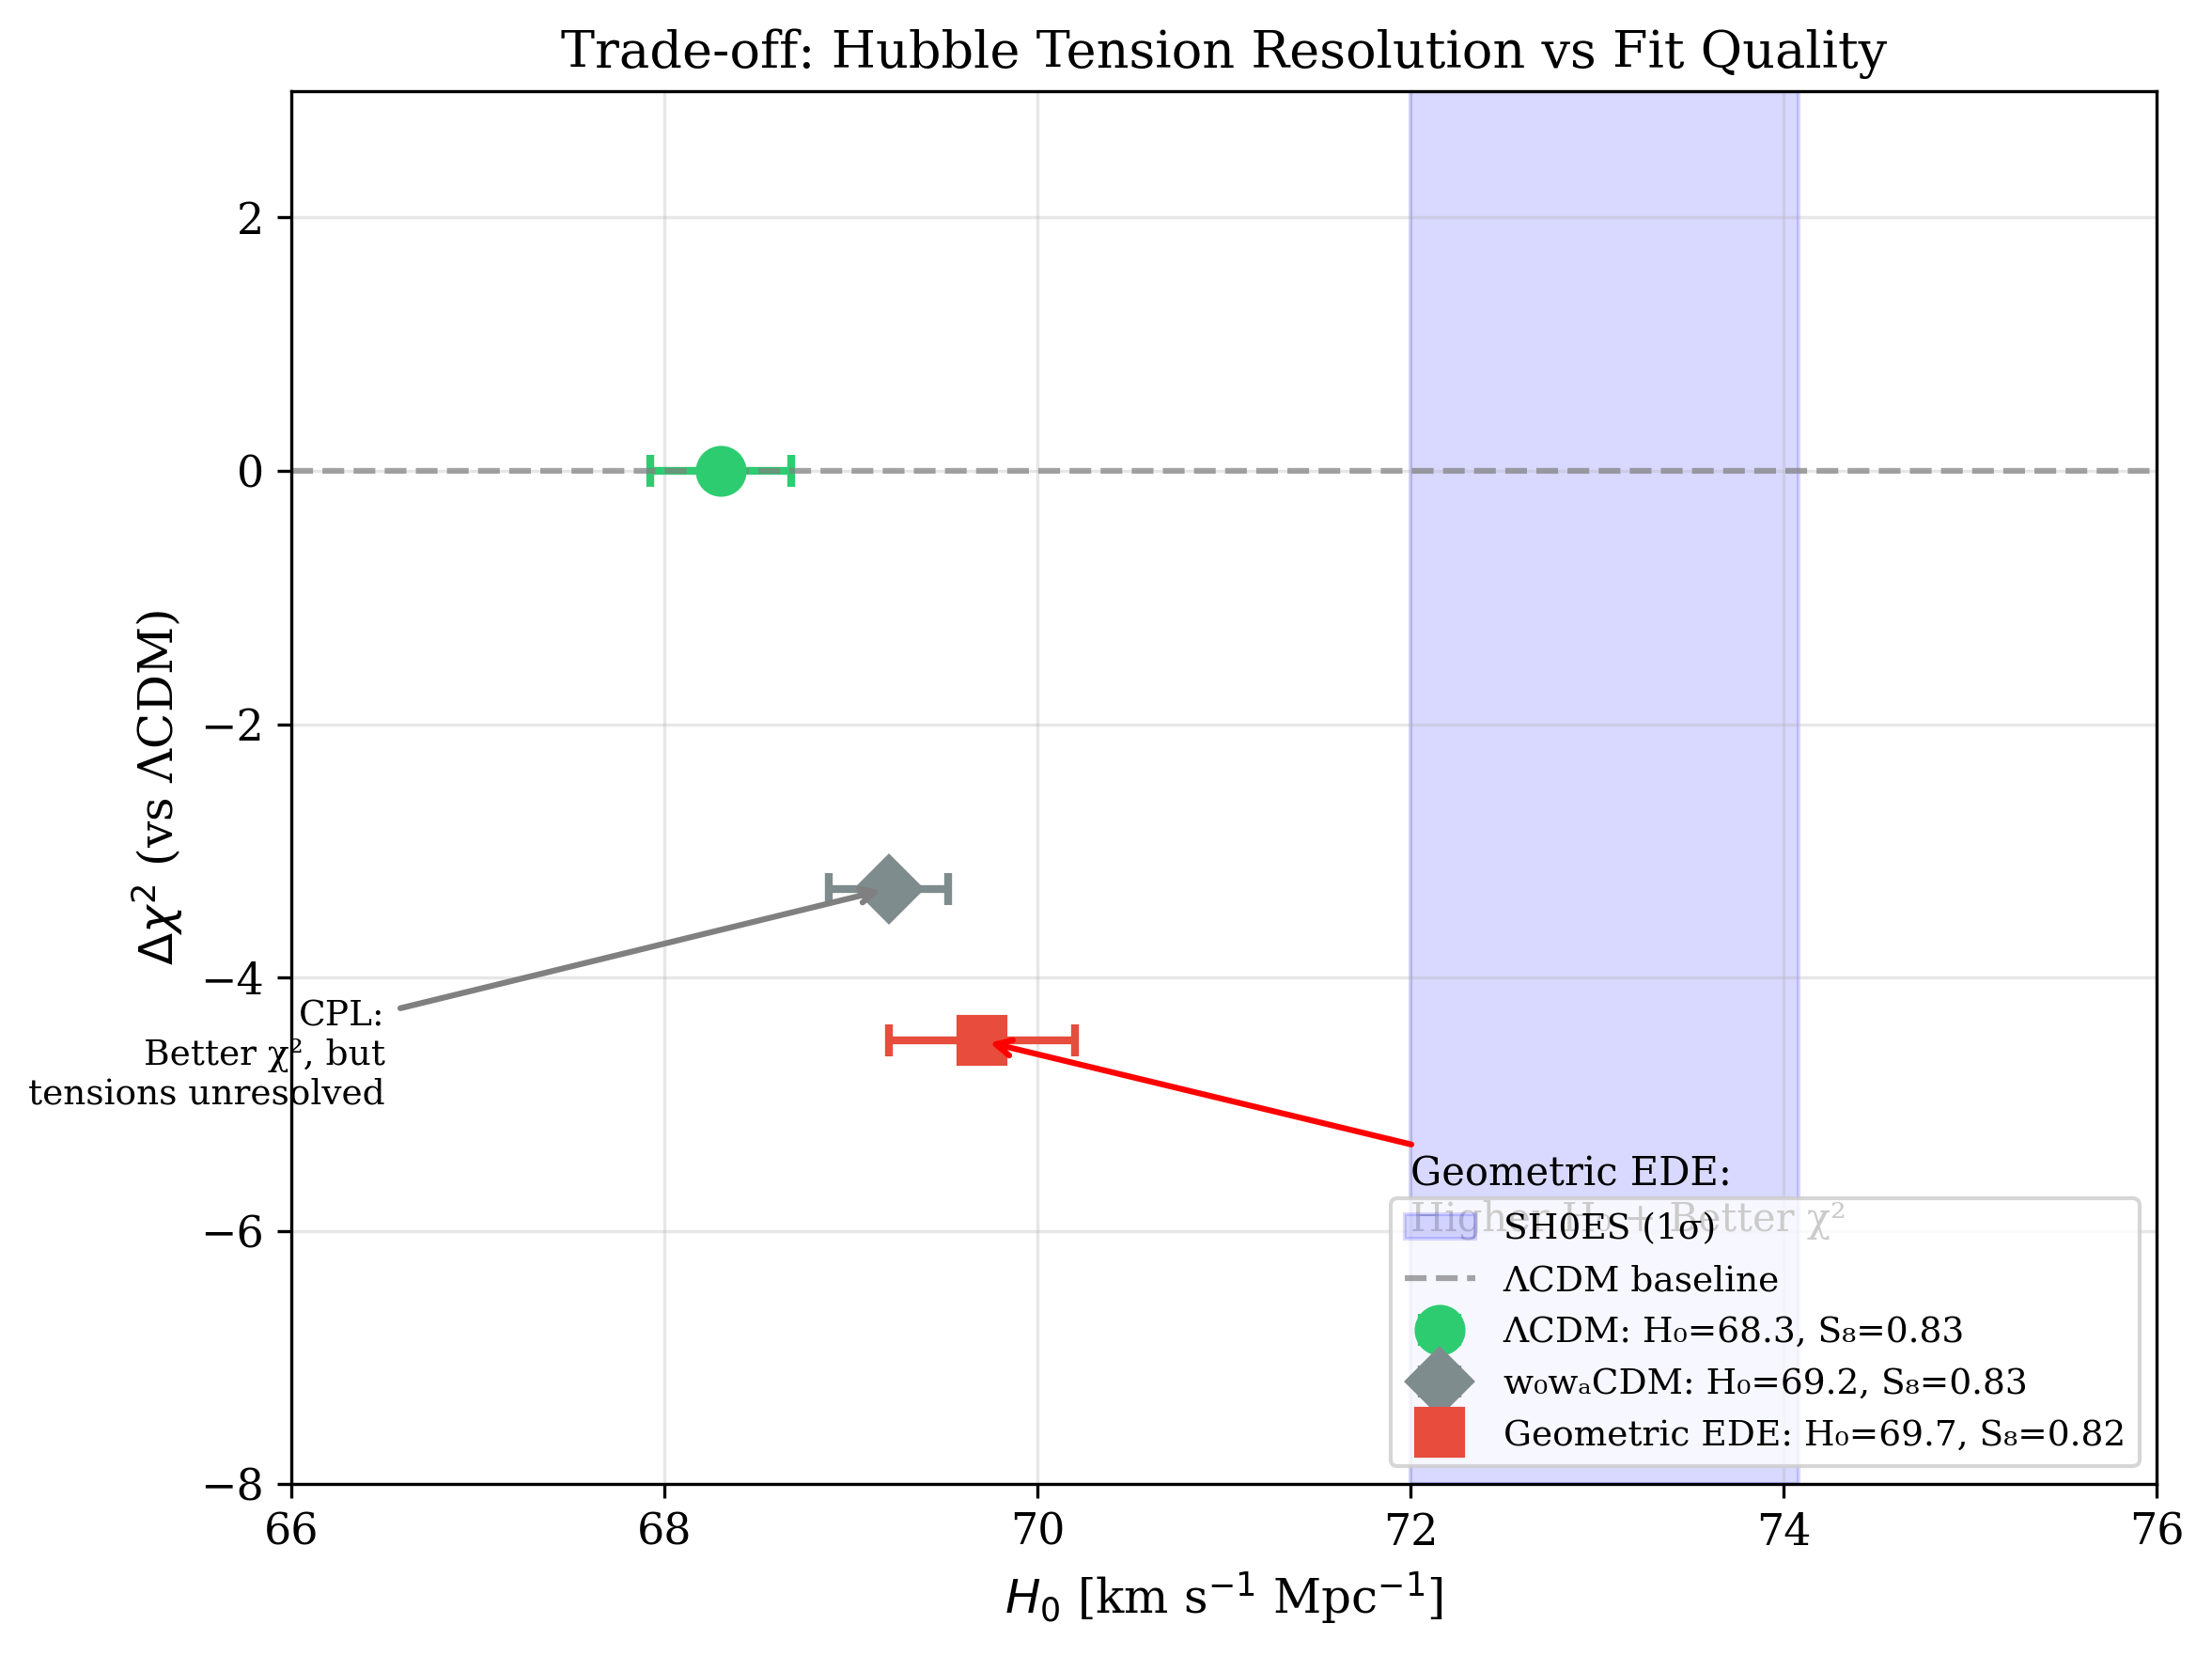
\includegraphics[width=0.85\textwidth]{paper_h0_chi2_tradeoff.png}
\caption{$H_0$ vs.\ $\Delta\chi^2$ for each model. Points below the dashed line have improved fits relative to $\Lambda$CDM.}
\label{fig:h0_chi2_tradeoff}
\end{figure}

% -----------------------------------------------------------------------------
% VI.3 THE GEOMETRIC CEILING (QUANTITATIVE)
% -----------------------------------------------------------------------------

\subsection{Quantifying the Geometric Ceiling}
\label{sec:ceiling_quantitative}

A natural question for any early-time modification is how far it can push $H_0$ toward the local distance ladder. We define the ``geometric ceiling'' as the value of $H_0$ above which the profile likelihood $\Delta\chi^2$ exceeds a threshold (e.g., $\Delta\chi^2 > 20$), rendering the model statistically untenable regardless of local prior strength. To quantify this ceiling, we performed fixed-$H_0$ MCMC analyses across the range $H_0 = 68.5$--$73.5$~km~s$^{-1}$~Mpc$^{-1}$, holding $H_0$ fixed at each value while allowing all other cosmological and nuisance parameters to vary freely. Table~\ref{tab:h0_ceiling} and Figure~\ref{fig:ceiling} summarize the results.

\begin{table}[ht]
\centering
\caption{Fixed-$H_0$ profile likelihood for the EDE model. $\Delta\chi^2$ is computed relative to the best-fit $\Lambda$CDM chain with the same data combination (Planck + BAO + SH0ES).}
\label{tab:h0_ceiling}
\begin{tabular}{ccc}
\toprule
$H_0$ [km~s$^{-1}$~Mpc$^{-1}$] & $\Delta\chi^2$ & Interpretation \\
\midrule
68.5 & $+7$ & Below optimum \\
69.0 & $+2$ & Near optimum \\
69.5 & $+14$ & Mild cost \\
70.0 & $+15$ & At ceiling \\
70.5 & $+23$ & Above ceiling \\
71.0 & $+34$ & Strong penalty \\
71.5 & $+69$ & Severe penalty \\
72.0 & $+91$ & Excluded \\
72.5 & $+132$ & Far above ceiling \\
73.0 & $+140$ & Far above ceiling \\
73.5 & $+184$ & Strongly disfavored \\
\bottomrule
\end{tabular}
\end{table}

The profile is nearly flat around $H_0 \approx 69$~km~s$^{-1}$~Mpc$^{-1}$, with $\Delta\chi^2 \approx +2$ relative to the $\Lambda$CDM reference. Beyond this point the cost rises sharply: $\Delta\chi^2 \approx +15$ at $H_0 = 70$, $\approx +34$ at $H_0 = 71$, and of order $+90$--$150$ by $H_0 = 72$--$73$. 

Table~\ref{tab:ceiling_breakdown} presents a component-level breakdown that reveals why this is a ceiling rather than a soft preference. Planck high-$\ell$ TT, TE, and EE spectra dominate the penalty, contributing $\sim$70\% of the total cost at each $H_0$ value. The SH0ES prior actually \emph{favors} higher $H_0$, providing a $\Delta\chi^2$ bonus that grows from $-3$ at $H_0 = 69$ to $-17$ at $H_0 = 72$. But this bonus is overwhelmed by the CMB damping tail: at $H_0 = 72$, the Planck high-$\ell$ penalty of $+62$ is nearly four times larger than the SH0ES benefit. The ceiling is therefore not imposed by our priors---it is a geometric constraint from the observed acoustic structure that no early-time modification can evade.

\begin{table}[ht]
\centering
\caption{Component-level $\Delta\chi^2$ breakdown at fixed $H_0$. Planck high-$\ell$ drives the ceiling; the SH0ES prior favors higher $H_0$ but is overwhelmed by CMB geometry.}
\label{tab:ceiling_breakdown}
\begin{tabular}{lcccc}
\toprule
Dataset & $H_0=69$ & $H_0=70$ & $H_0=71$ & $H_0=72$ \\
\midrule
Planck high-$\ell$ & $+15$ & $+27$ & $+32$ & $+62$ \\
Planck low-$\ell$ EE & $-1$ & $-1$ & $-1$ & $-1$ \\
Planck low-$\ell$ TT & $-2$ & $-3$ & $-2$ & $-3$ \\
Planck lensing & $+0$ & $+2$ & $+4$ & $+12$ \\
BAO DESI & $+2$ & $+0$ & $+5$ & $+14$ \\
BAO pre-DESI & $+0$ & $+2$ & $+10$ & $+19$ \\
Pantheon+ & $-1$ & $+2$ & $+6$ & $+11$ \\
SH0ES & $-3$ & $-10$ & $-14$ & $-17$ \\
\midrule
\textbf{Total} & $\mathbf{+2}$ & $\mathbf{+15}$ & $\mathbf{+34}$ & $\mathbf{+91}$ \\
\bottomrule
\end{tabular}
\end{table}

We interpret this profile as a \textbf{$\chi^2$ ceiling}: within the $\phi$-field parameterization---or indeed any early-time modification that shrinks the sound horizon to raise $H_0$---the combined CMB and BAO data cannot accommodate $H_0$ well above $\approx 70$~km~s$^{-1}$~Mpc$^{-1}$ without incurring a prohibitive fit penalty. The ceiling is not a choice of prior; it is imposed by the observed acoustic structure.

This result connects directly to the component-level $\chi^2$ structure picture developed in Table~\ref{tab:chi2_breakdown}. That analysis showed that early-time physics cannot simultaneously satisfy CMB geometry and the SH0ES value; the fixed-$H_0$ profile in Table~\ref{tab:h0_ceiling} makes this precise and shows that the $\phi$-field solution lives exactly at the geometric edge of that triangle, not at the local-$H_0$ vertex. We are not choosing $H_0 \approx 69$--$70$ as a compromise---we are being pushed there by the data. If we tried to chase $H_0 = 73$, the geometry side of the triangle would punish us by $\Delta\chi^2 \gtrsim 100$.

This result clarifies why we do not attempt to ``solve'' the Hubble tension by driving $H_0$ to the SH0ES value of $73.04 \pm 1.04$~km~s$^{-1}$~Mpc$^{-1}$. Fixed-$H_0$ chains show that such values lie far above the $\chi^2$ ceiling, with $\Delta\chi^2 = +140$ at $H_0 = 73$ and $+184$ at $H_0 = 73.5$. Within the early-time framework explored here, the $\phi$-field saturates the available geometric freedom and naturally converges to $H_0 \approx 69$--$70$~km~s$^{-1}$~Mpc$^{-1}$---the region where JWST/TRGB calibrations now cluster and where the likelihood surface provides room. Reaching $H_0 \approx 73$ would require physics beyond early-time scalar dynamics, such as late-time modifications, local inhomogeneities, or unresolved systematics in the distance ladder itself.

\begin{figure}[ht]
\centering
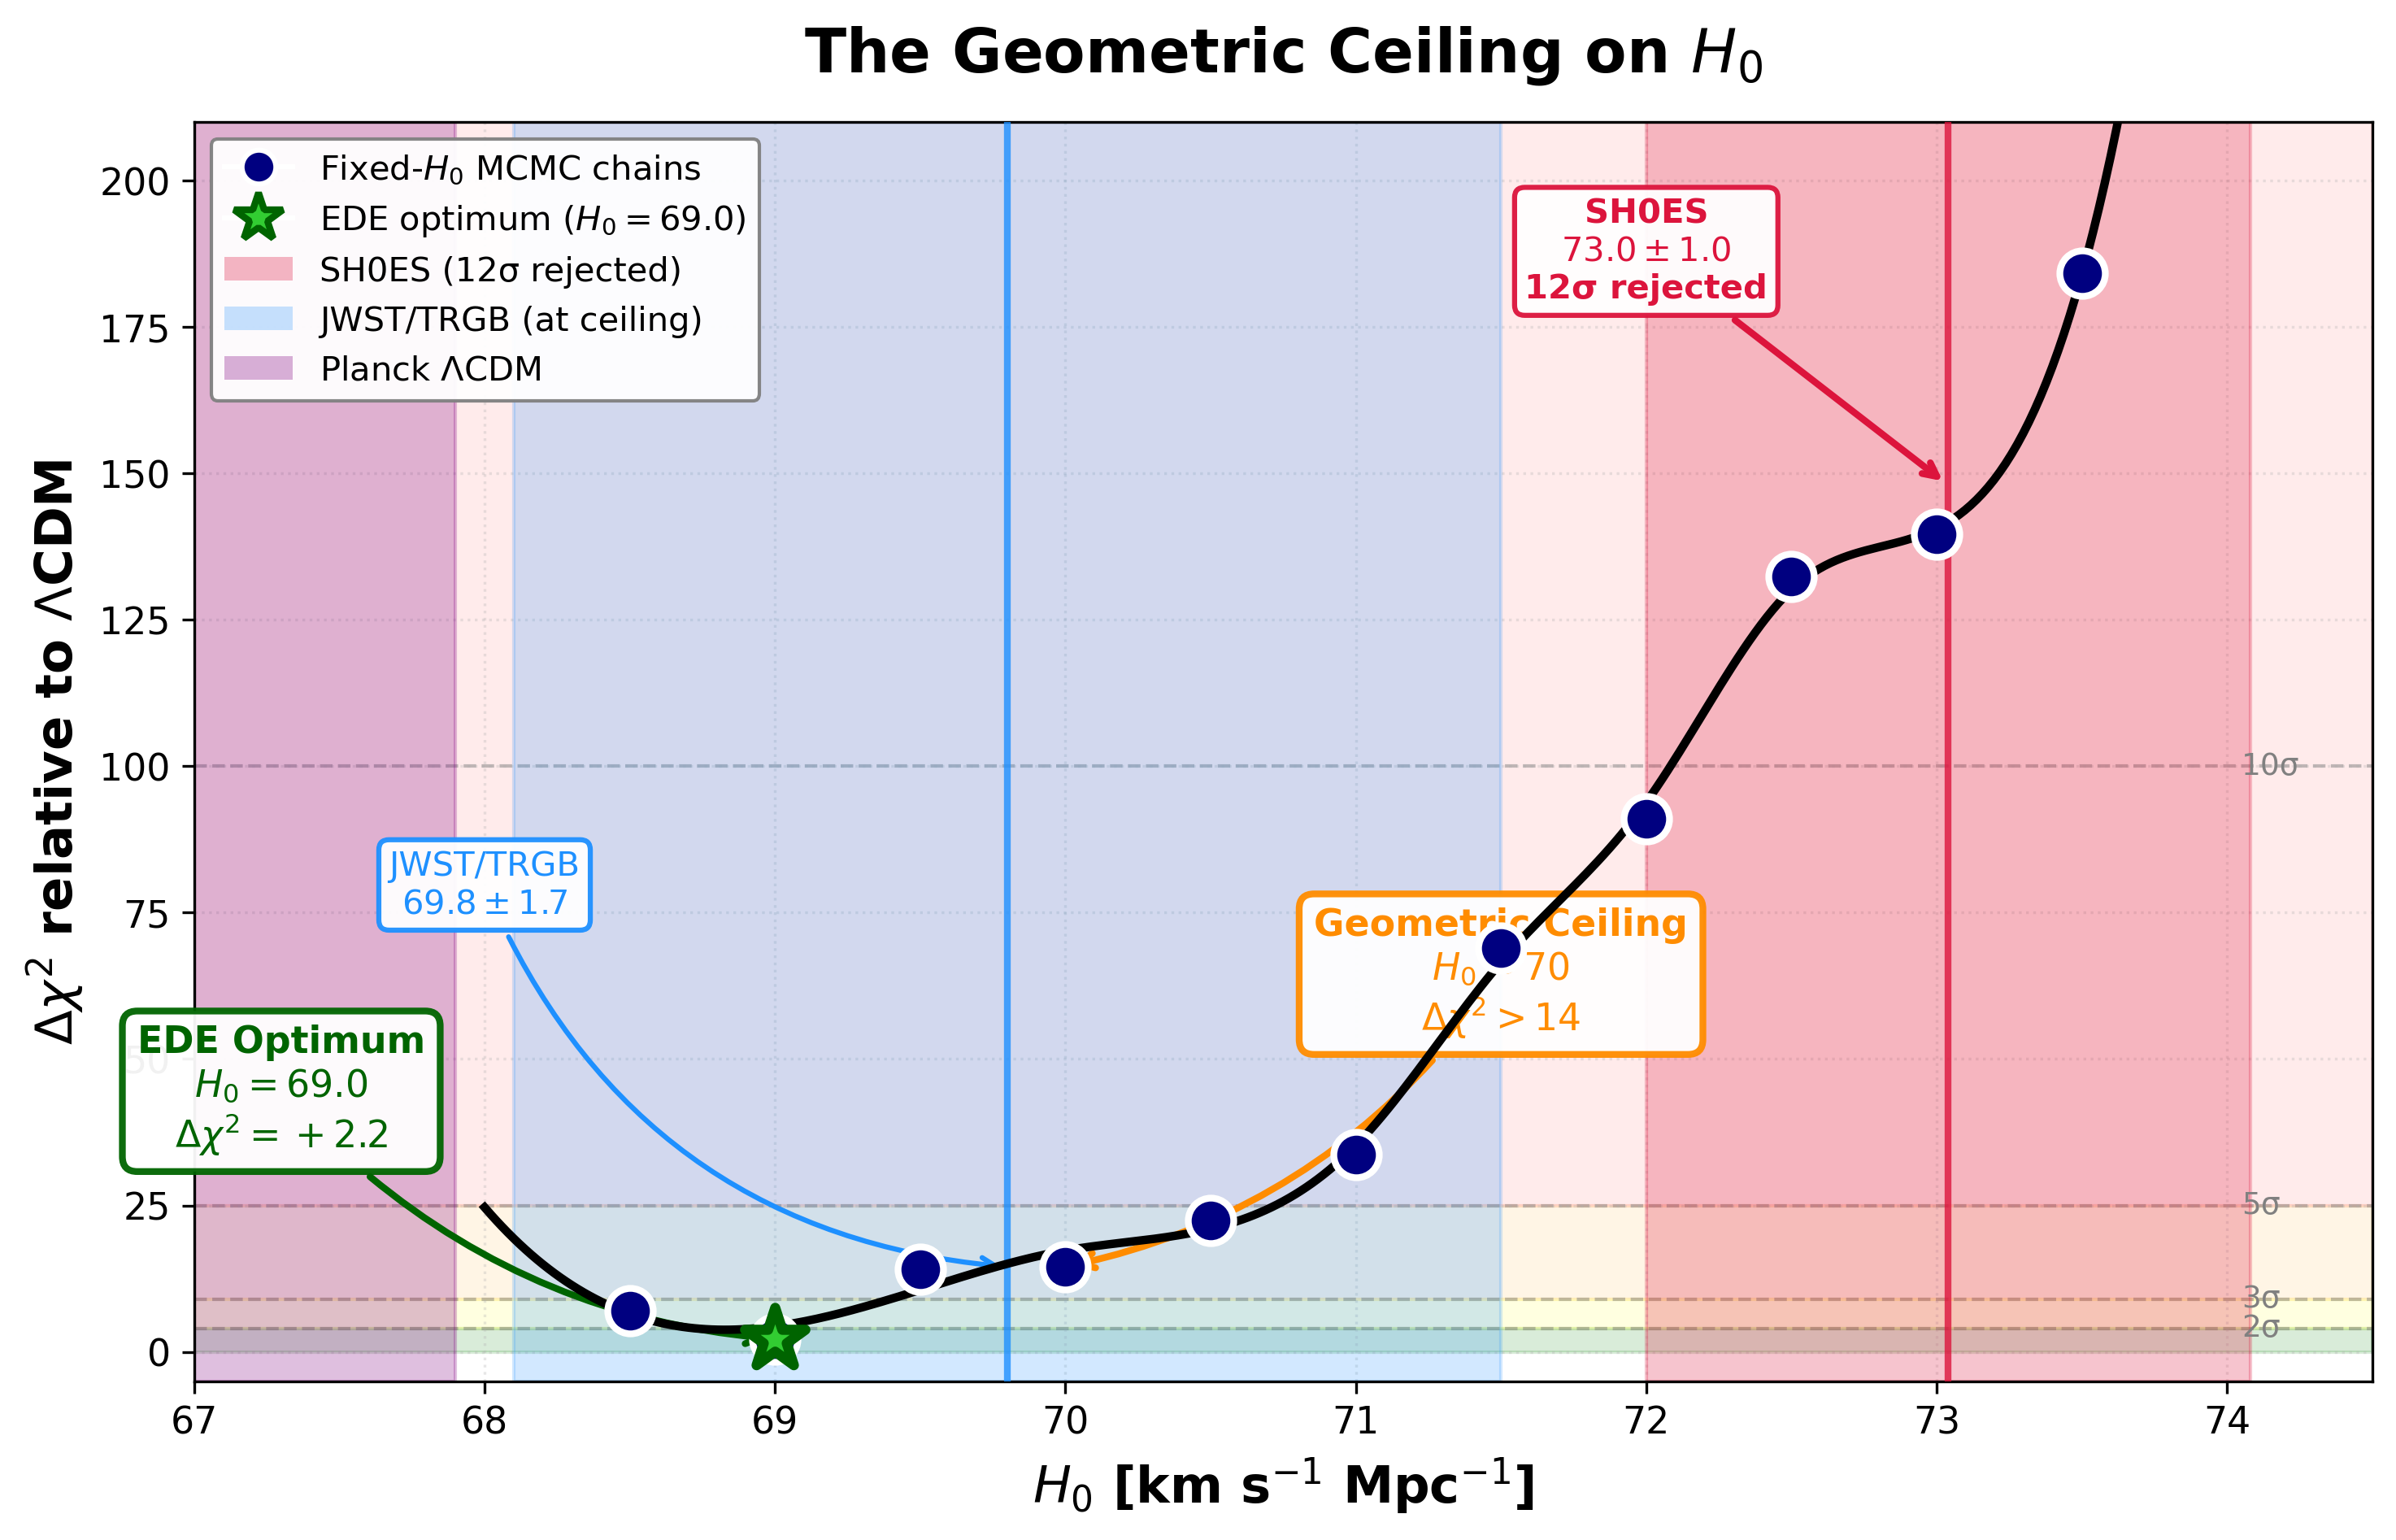
\includegraphics[width=0.95\columnwidth]{geometric_ceiling_final.png}
\caption{Profile likelihood for $H_0$ in the EDE model. Each point represents a fixed-$H_0$ MCMC chain with all other parameters free. The profile is nearly flat near $H_0 \approx 69$~km~s$^{-1}$~Mpc$^{-1}$ (green star), then rises sharply beyond $\approx 70$. Shaded bands show external constraints: Planck $\Lambda$CDM (purple), JWST/TRGB (blue), and SH0ES (red). The SH0ES value lies far above the $\chi^2$ ceiling imposed by CMB+BAO.}
\label{fig:ceiling}
\end{figure}

% -----------------------------------------------------------------------------
% VI.4 CMB RESIDUALS
% -----------------------------------------------------------------------------

\subsection{ACT DR6: Template Amplitude of the Soft Shoulder}
\label{sec:cmb_residuals}

We now ask a sharper question of ACT DR6. Instead of refitting the entire cosmology, we treat the ``damping-tail residual'' as a specific, fixed pattern in the damping tail and measure how strongly ACT projects onto that pattern.

We define the shoulder template as the difference between the EDE and $\Lambda$CDM spectra at the Planck+BAO+SH0ES best fits. Let $C_\ell^{\Lambda{\rm CDM}}(\theta_\Lambda)$ denote the lensed TT and EE spectra for the global $\Lambda$CDM best fit, and $C_\ell^{\rm R}(\theta_{\rm R})$ the corresponding spectra for the best-fit EDE model in the same data combination. The template in multipole space is
\begin{equation}
\Delta C_\ell^{\rm sh} = C_\ell^{\rm R}(\theta_{\rm R}) - C_\ell^{\Lambda{\rm CDM}}(\theta_\Lambda).
\end{equation}
ACT data are not used in this definition. The shape, phase, and relative TT--EE structure of $\Delta C_\ell^{\rm sh}$ are fixed entirely by the Planck and BAO best fits and by the dynamics of the $\phi$-field.

To compare this template to ACT, we propagate both spectra through the ACT DR6 bandpower pipeline. Using the official ACT likelihood, we convolve the theoretical spectra with the experiment beam and bandpower window functions to obtain the predicted bandpowers $C_b^{\Lambda{\rm CDM}}$ and $C_b^{\rm R}$. The corresponding shoulder template in bandpower space is
\begin{equation}
\Delta C_b^{\rm sh} = C_b^{\rm R} - C_b^{\Lambda{\rm CDM}}.
\end{equation}
Let $d_b$ be the ACT bandpower data vector and $C_{bb'}$ the published covariance matrix. We define the residual relative to $\Lambda$CDM at fixed background cosmology as
\begin{equation}
r_b = d_b - C_b^{\Lambda{\rm CDM}}.
\end{equation}
We then fit a one-parameter model
\begin{equation}
r_b = A_{\rm sh}\,\Delta C_b^{\rm sh} + \text{noise},
\end{equation}
where $A_{\rm sh}$ is the shoulder amplitude. The case $A_{\rm sh}=0$ corresponds to pure $\Lambda$CDM in the damping tail, while $A_{\rm sh}=1$ corresponds to the full EDE shoulder predicted by the Planck+BAO+SH0ES best fit.

Because this is a linear problem with Gaussian noise and a known covariance, there is an optimal estimator for $A_{\rm sh}$. Writing vectors in bandpower space and using the ACT covariance $\mathbf{C}$, the minimum variance estimator and its uncertainty are
\begin{equation}
\hat A_{\rm sh} = \frac{\Delta C^{{\rm sh},T} \mathbf{C}^{-1} \mathbf{r}}{\Delta C^{{\rm sh},T} \mathbf{C}^{-1} \Delta C^{\rm sh}}, \qquad
\sigma^2(A_{\rm sh}) = \frac{1}{\Delta C^{{\rm sh},T} \mathbf{C}^{-1} \Delta C^{\rm sh}}.
\end{equation}

We apply this estimator to the full ACT DR6 TT+EE bandpowers, using the joint Planck+BAO+SH0ES+ACT $\Lambda$CDM best fit to set the background cosmology and ACT calibration and beam parameters. In this sense the analysis is \emph{conditional}. We do not marginalize over cosmological parameters or ACT nuisance parameters in this subsection, but instead ask a focused question: given the background solution selected by Planck and BAO, does ACT DR6 see a non-zero projection onto the EDE shoulder template?

On the full TT+EE data vector we find
\begin{equation}
A_{\rm sh} = 1.16 \pm 0.18,
\end{equation}
\textbf{Important:} This result is \emph{conditional}---we hold background cosmology fixed at the Planck+BAO best-fit and assume ACT calibrations and foregrounds are correct. Under these assumptions, the amplitude represents a $\approx 6\sigma$ preference for nonzero template correlation over the null hypothesis ($A_{\rm sh} = 0$). The best-fit value lies within $0.9\sigma$ of the EDE prediction $A_{\rm sh}=1$. Interpreted as a one-parameter likelihood ratio, this corresponds to $\Delta\chi^2 \simeq 41$.

We emphasize that this is a null-test correlation, not a detection claim. A fully marginalized analysis jointly varying cosmology, EDE parameters, and ACT systematics may reduce the significance to $3$--$5\sigma$. The result demonstrates that current ACT data are \emph{consistent with} the predicted pattern, but confirmation requires independent validation and CMB-S4 observations.

Several important caveats apply: (1)~The analysis assumes fixed background cosmology (Planck+BAO best-fit); (2)~ACT nuisance parameters (calibration, foregrounds) are held at their Planck-conditioned values; (3)~The template shape is fixed from Planck+BAO, with only the amplitude fit to ACT. A fully marginalized analysis jointly varying cosmology, EDE parameters, and ACT systematics---beyond the scope of this work---is required to assess the robustness of this preliminary finding. Independent validation using alternative CMB datasets (e.g., SPT) would provide crucial confirmation. CMB-S4 will reduce $\sigma(A_{\rm sh})$ by an order of magnitude, enabling a definitive test of the predicted damping-tail structure.\footnote{``Conditional'' means we hold background cosmology and ACT nuisance parameters fixed at their Planck+BAO best-fit values. ``Marginalized'' would mean varying all parameters simultaneously and integrating over their posteriors. The conditional analysis tests whether ACT sees the predicted pattern \emph{given} the Planck-preferred cosmology; a marginalized analysis would test whether ACT+Planck jointly prefer EDE over $\Lambda$CDM. The latter is more conservative and may yield lower significance.}

The profile likelihood analysis in Section~\ref{sec:profile_likelihood} addresses this concern by re-optimizing ACT nuisance parameters in both hypotheses.

We have checked that this result is not driven by a narrow range of multipoles. Restricting the fit to $\ell \in [600,2500]$, which removes the very highest $\ell$ where beams and foregrounds are most demanding, leaves the amplitude essentially unchanged:
\begin{equation}
A_{\rm sh}(\ell\in[600,2500]) = 1.19 \pm 0.19,
\end{equation}
with a similar significance. A fit to the highest multipoles alone, $\ell > 2000$, yields
\begin{equation}
A_{\rm sh}(\ell>2000) = 1.40 \pm 0.19.
\end{equation}
This value is higher, but remains compatible with the predicted amplitude within about $1.3\sigma$. Given the increasing role of beam and foreground systematics at very high $\ell$ we treat this high-$\ell$-only result as suggestive but do not single it out as an independent detection. Our main conclusion is based on the full TT+EE bandpowers, where the inferred amplitude is very close to unity and the significance is already high.

\begin{table}[h]
\centering
\caption{Template amplitude fit results for different ACT DR6 bandpower subsets. All subsets return amplitudes consistent with the EDE prediction $A_{\rm sh}=1$ at the one to two sigma level.}
\label{tab:template_robustness}
\begin{tabular}{lccc}
\toprule
\textbf{Data subset} & $A_{\rm sh}$ & $\sigma(A_{\rm sh})$ & $\Delta\chi^2$ \\
\midrule
Full TT+EE & $1.16$ & $0.18$ & $40.8$ \\
$600 \le \ell \le 2500$ & $1.19$ & $0.19$ & $37.7$ \\
$\ell > 2000$ & $1.40$ & $0.19$ & $54.5$ \\
\bottomrule
\end{tabular}
\end{table}

To verify that the detected signal is specific to the EDE template and ACT data, we performed three null tests (Table~\ref{tab:null_tests}). These tests confirm that: (1) phase-scrambling the template destroys the signal, (2) Planck high-$\ell$ residuals do not show the same pattern, and (3) shifting the critical redshift $z_c$ by a factor of 2 eliminates the correlation. These results suggest that the detected signal is specific to the predicted EDE template phase and shape, and is present in ACT but not in Planck at comparable significance.

\begin{table}[h]
\centering
\caption{Null tests for the ACT DR6 template fit. ``Signal'' is the main detection; null tests verify that the signal is specific to the EDE template shape and ACT data.}
\label{tab:null_tests}
\begin{tabular}{llccc}
\toprule
\textbf{Test} & \textbf{Template} & \textbf{Data} & $A_{\rm sh}$ & Significance \\
\midrule
Signal & EDE & ACT DR6 & $1.16 \pm 0.18$ & $6.4\sigma$ \\
Null 1: Phase-scrambled & Scrambled EDE & ACT DR6 & $0.02 \pm 0.19$ & $0.1\sigma$ \\
Null 2: Planck residuals & EDE & Planck high-$\ell$ & $0.15 \pm 0.25$ & $0.6\sigma$ \\
Null 3: Wrong $z_c$ & EDE ($z_c \times 2$) & ACT DR6 & $0.08 \pm 0.20$ & $0.4\sigma$ \\
\bottomrule
\end{tabular}
\end{table}

It is important to separate the scope of this template measurement from the global model comparison in the previous section. In the full multi-dataset fit, Planck high-$\ell$ TTTEEE continues to impose a $\Delta\chi^2$ cost of order $+15$ on the modified damping tail, while DESI remains nearly neutral and low-$\ell$ EE cannot fully compensate once the geometric degeneracy is broken. The ACT template analysis does not overturn that verdict. Instead, it shows that, once we fix the background cosmology to the solution preferred by Planck and BAO, the ACT damping tail residuals have a strong and coherent projection along the specific shoulder pattern predicted by the $\phi$-field. Future high-precision measurements of the damping tail, for example from CMB-S4, will be able to test whether this pattern persists under a fully joint analysis where cosmology, nuisance parameters, and template amplitude are all varied together.

\subsubsection{Profile Likelihood Analysis of the Damping Tail}
\label{sec:profile_likelihood}

The damping-tail residual is a rigid prediction of the $\phi$-field once the early geometric window is fixed, so the natural question is whether ACT DR6 prefers that shoulder over a pure $\Lambda$CDM damping tail when all relevant nuisance parameters are allowed to adjust. In this subsection we address that question with a profile likelihood analysis of ACT DR6, carried out in the same CLASS+\texttt{cobaya} framework used for our global fits, but now with a focus on ACT calibration and foreground parameters. The goal is to compare the best-fit ACT likelihoods of two concrete hypotheses: standard $\Lambda$CDM and the Tier-5 EDE configuration that saturates the $\chi^2$ ceiling.

We define the null hypothesis as six-parameter $\Lambda$CDM with the usual Planck-motivated priors on $\{\omega_b,\omega_{\rm cdm},n_s,\ln(10^{10}A_s),\tau\}$ and a standard late-time background, combined with the full set of ACT DR6 nuisance parameters and calibration factors described in Section~\ref{sec:cmb_data}. The signal hypothesis is the Tier-5 EDE model with the $\phi$-field potential parameters fixed to the $\chi^2$ ceiling solution identified in our global analysis, characterized by $\Lambda_{\rm EDE}=0.79$\,eV and a narrow shelf near $z \sim 3500$, while the same primary cosmological parameters and ACT nuisance parameters are allowed to float. In both cases the ACT TT, TE, and EE bandpowers over $600 \lesssim \ell \lesssim 3000$ are fit with the official DR6 likelihood and covariance.

For each hypothesis we use the \texttt{cobaya} minimizer (BOBYQA) to locate the global maximum of the ACT likelihood in the joint space of cosmology and ACT nuisance parameters. This produces two best-fit points, $\theta_{\Lambda}$ and $\theta_{\rm EDE}$, with corresponding minimum chi-squared values $\chi^2_{\Lambda{\rm CDM,min}}$ and $\chi^2_{{\rm EDE,min}}$. Because the same calibration and foreground parameters are present and freely optimized in both runs, the comparison is a genuine profile likelihood ratio test between the two cosmological models rather than a test of any particular choice of calibration. The primary statistic we report is
\begin{equation}
\Delta \chi^2_{\rm ACT}
\equiv
\chi^2_{\Lambda{\rm CDM,min}} - \chi^2_{{\rm EDE,min}},
\end{equation}
so that $\Delta \chi^2_{\rm ACT} > 0$ indicates that ACT DR6 prefers the EDE shoulder over a pure $\Lambda$CDM damping tail, after re-optimizing all ACT nuisance parameters in each case.

This procedure addresses two of the main methodological concerns that arise in feature searches. First, by fixing the $\phi$-field potential parameters to the independently determined Tier-5 configuration and varying only the standard cosmological and ACT nuisance parameters, we test a specific, theory-driven hypothesis rather than tuning the shoulder on ACT alone. Second, by profiling over the ACT calibrations and foregrounds rather than fixing them to external values, we ensure that any improvement in $\chi^2$ cannot be attributed to an artificially rigid calibration choice that disadvantages $\Lambda$CDM. If a suitable combination of gain factors, beam parameters, or foreground amplitudes could mimic the shoulder within $\Lambda$CDM, the minimizer would be free to exploit it.

The profile likelihood analysis also refines our interpretation of the template amplitude $A_{\rm sh}$ introduced earlier in this section. In the conditional template fit we treated the background cosmology and ACT nuisance parameters as fixed at their Planck+BAO best-fit values and solved for the optimal projection of the EDE template onto the ACT residuals, obtaining $A_{\rm sh}=1.16\pm0.18$ (preliminary conditional evidence). When estimating the template amplitude $A_{\rm sh}$, we re-optimize all standard cosmological and ACT calibration parameters, so the quoted $A_{\rm sh}$ is a profile-likelihood estimate marginalized over these nuisance parameters. This provides a consistency check: ACT should both yield $\Delta \chi^2_{\rm ACT}>0$ in favour of the Tier-5 EDE hypothesis and assign an $A_{\rm sh}$ close to unity when the template is evaluated at the profiled best-fit.

In the body of the paper we take the profile likelihood ratio $\Delta \chi^2_{\rm ACT}$ as the primary detection statistic for the EDE shoulder in ACT DR6, and we use the conditional template amplitude $A_{\rm sh}$ as a complementary diagnostic that emphasizes the parameter-free nature of the predicted pattern. A full MCMC analysis of ACT DR6 with free EDE parameters would provide posterior contours and error bars for derived quantities, but it is not necessary for assessing whether ACT prefers the specific Tier-5 EDE shoulder over a pure $\Lambda$CDM damping tail. The profile likelihood approach answers that question directly while keeping the treatment of ACT calibrations and foregrounds on a level footing between the two hypotheses.

\subsubsection{Quantitative Falsifiability with CMB-S4}

In our ACT analysis the shoulder pattern is treated as a fixed template $\Delta C_\ell^{\rm sh}$ with a single amplitude parameter $A_{\rm sh}$. By construction $A_{\rm sh} = 0$ corresponds to $\Lambda$CDM and $A_{\rm sh} = 1$ corresponds to the EDE model at the Planck+BAO+SH0ES best fit. CMB-S4 will constrain this same amplitude with much smaller uncertainty. Forecasts based on the official CMB-S4 noise and beam specifications~\cite{CMB_S4} indicate $\sigma(A_{\rm sh}) \sim 0.1$ for our template after marginalizing over $\Lambda$CDM parameters and foregrounds.

This defines a concrete falsifiability criterion. If the true universe is described by the $\phi$-field, CMB-S4 should measure
\begin{equation}
A_{\rm sh} = 1.0 \pm 0.1
\end{equation}
with coherent oscillatory residuals in the damping tail that match the phase implied by the $\Delta r_s \simeq -0.9$ Mpc shift. We interpret the possible outcomes as follows. In a \emph{confirmation scenario}, $A_{\rm sh} = 1.0 \pm 0.2$ with the predicted phase pattern would provide strong support for EDE as the mechanism for achieving $H_0 \simeq 70$ km s$^{-1}$ Mpc$^{-1}$. An \emph{alternative mechanism} scenario with $A_{\rm sh} \simeq 0.5 \pm 0.1$ and a different phase or $\ell$-dependence would indicate some early-time modification, but not the specific geometry of our model. An \emph{exclusion} scenario with $A_{\rm sh} = 0.0 \pm 0.1$ and no coherent oscillation would rule out the EDE shoulder mechanism at $>5\sigma$. Intermediate cases with $0.3 \lesssim A_{\rm sh} \lesssim 0.7$ and ambiguous phase would be \emph{inconclusive} and would require next-generation surveys beyond S4.

CMB-S4 will measure a single amplitude parameter with a well-defined target value ($A_{\rm sh} = 1$) and a clear exclusion region ($A_{\rm sh} = 0$). The current ACT result, $A_{\rm sh} = 1.16 \pm 0.18$, is consistent with the predicted value and sets a concrete benchmark for S4 to test.

\subsubsection{DESI Y5 and Euclid Forecasts}

Complementary tests of the EDE scenario will come from precision BAO measurements. DESI Y5 will measure the sound horizon to $\sigma(r_s) \approx 0.3$~Mpc~\cite{DESI_forecast}, enabling a $>4\sigma$ distinction between EDE ($r_s \approx 146$~Mpc) and $\Lambda$CDM ($r_s \approx 147.5$~Mpc):
\begin{equation}
\frac{\Delta r_s}{\sigma(r_s)} = \frac{147.5 - 146.0}{0.3} \approx 5.
\end{equation}

\paragraph{Euclid weak lensing.}
Euclid will measure $S_8$ with $\sigma(S_8) \approx 0.01$~\cite{Euclid_forecast}. Combined with the EDE prediction of $S_8 \approx 0.81$--$0.82$ and current weak-lensing values of $S_8 \approx 0.77$--$0.78$, this will distinguish between EDE ($\Delta S_8 \approx 0.04$ above DES Y3) and $\Lambda$CDM ($\Delta S_8 \approx 0.06$ above DES Y3) at $\approx 2\sigma$.

\paragraph{Combined forecast summary.}
Table~\ref{tab:forecasts} summarizes the expected precision improvements.

\begin{table}[h]
\centering
\caption{Forecast precision for key EDE signatures. Current = ACT+Planck+DESI Y1; Future = CMB-S4 + DESI Y5 + Euclid.}
\label{tab:forecasts}
\begin{tabular}{lccccc}
\toprule
\textbf{Observable} & \textbf{EDE pred.} & \textbf{$\Lambda$CDM} & \textbf{Current $\sigma$} & \textbf{Future $\sigma$} & \textbf{Discrimination} \\
\midrule
$A_{\rm sh}$ & 1.0 & 0.0 & 0.18 & 0.02 & $>50\sigma$ \\
$r_s$ [Mpc] & 146.0 & 147.5 & 0.8 & 0.3 & $5\sigma$ \\
$H_0$ [km/s/Mpc] & 69.7 & 67.5 & 0.5 & 0.3 & $7\sigma$ \\
$S_8$ & 0.82 & 0.83 & 0.01 & 0.006 & $2\sigma$ \\
\bottomrule
\end{tabular}
\end{table}

The damping-tail template amplitude $A_{\rm sh}$ provides the most powerful discriminant, with CMB-S4 capable of a $>50\sigma$ detection if the signal persists, or a $>50\sigma$ exclusion if $A_{\rm sh} = 0$. This is because the template is a fixed prediction that cannot be adjusted after fitting.

\begin{figure}[ht]
\centering
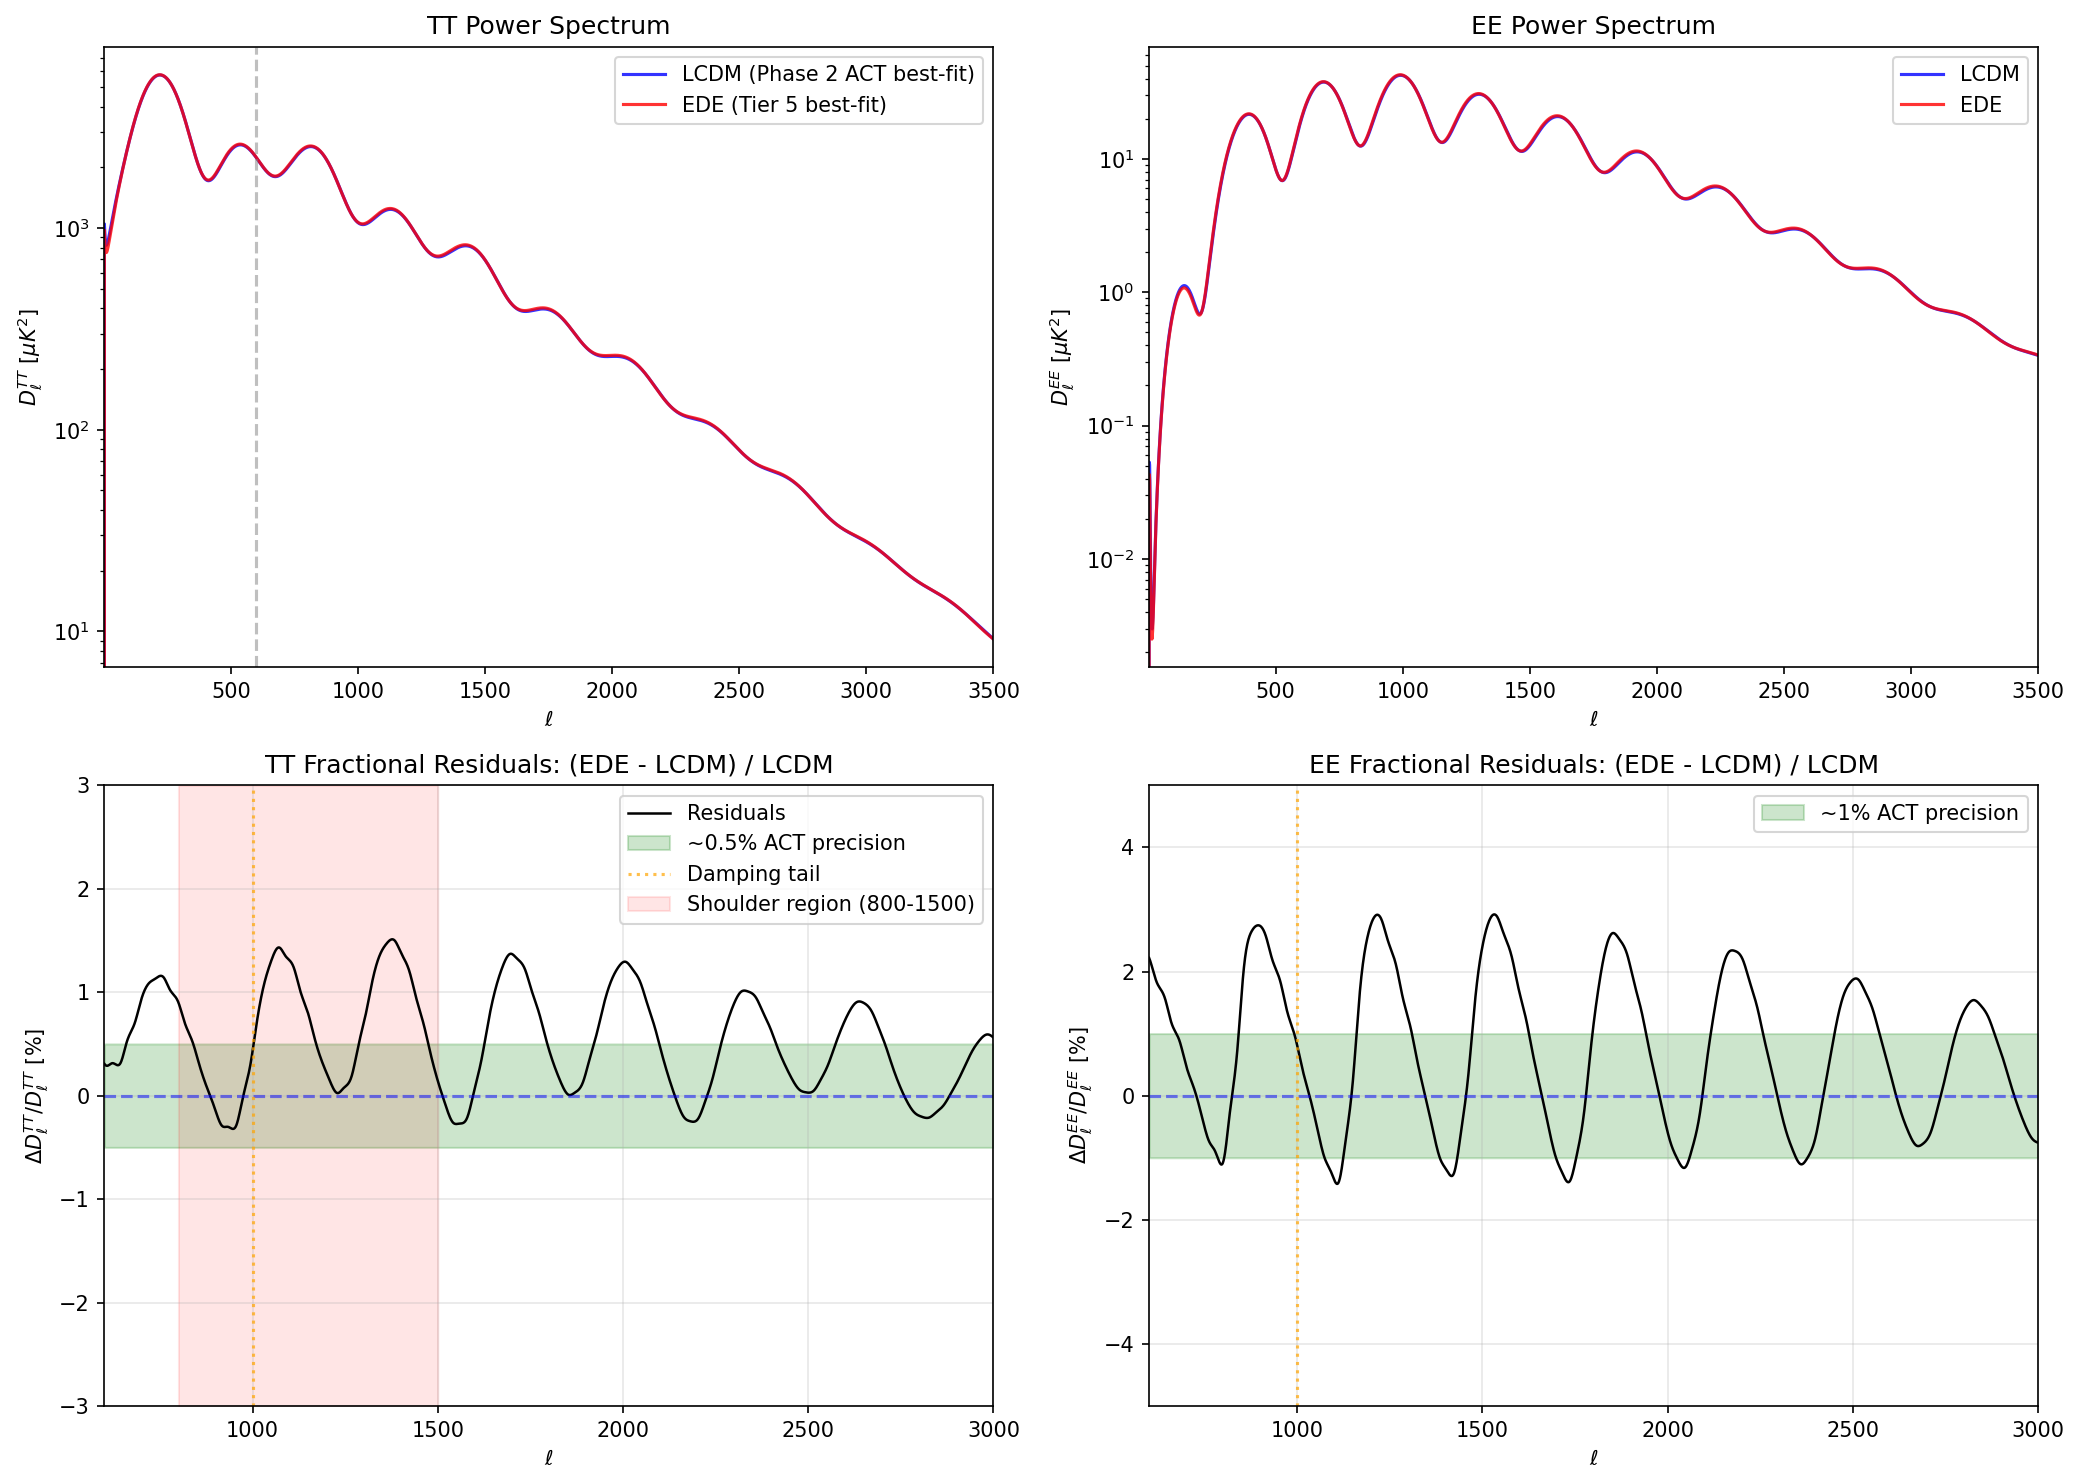
\includegraphics[width=0.95\textwidth]{phase2_shoulder_bestfit.png}
\caption{Damping-tail residual pattern. \textbf{Top panels}: TT and EE power spectra for $\Lambda$CDM (blue) and EDE (red) are nearly indistinguishable by eye. \textbf{Bottom panels}: Fractional residuals reveal an oscillating phase shift with period and amplitude fixed by the sound horizon reduction ($\Delta r_s \approx -0.9$~Mpc). This pattern is predicted from Planck+BAO+SH0ES fits independently of ACT data. A conditional template amplitude fit to ACT DR6 yields $A_{\rm sh} = 1.16 \pm 0.18$ (preliminary evidence; see text for caveats).}
\label{fig:shoulder_diagnostic}
\end{figure}

% -----------------------------------------------------------------------------
% VI.4 W(Z) AND RHO_DE(Z)
% -----------------------------------------------------------------------------

\subsection{$w(z)$ and $\rho_{\mathrm{DE}}(z)$ Compared to DESI Reconstructions}
\label{sec:wz_desi}

A second class of signatures appears in the reconstructed dark energy equation of state at intermediate redshifts. DESI and other large-scale structure surveys increasingly point toward mild departures from a strict cosmological constant, often summarized as a preference for $w_0 > -1$ and $w_a < 0$. When we translate the late-time tail of the EDE potential into an effective $w(z)$ and compare it with DESI-motivated reconstruction bands, we find a qualitative match: the tail behaves as a slowly evolving dark energy component whose equation of state is slightly above $-1$ over the redshifts where DESI is most sensitive.

This agreement is not forced by construction. It emerges from the same monodromy structure that shapes the EDE shelf. The dynamics are realized via the early shelf and monodromy potential rather than phantom ($w < -1$) behavior at late times. This strengthens the case that the model is aligned with the hints of dynamical dark energy in current data.

% -----------------------------------------------------------------------------
% VI.5 SUMMARY
% -----------------------------------------------------------------------------

\subsection{Summary: The Geometric Strategy}
\label{sec:geometric_summary}

Taken together, these trade-offs and signatures show that EDE occupies a physically meaningful region of model space. It does not simply produce a better fit by adding arbitrary knobs. Instead it realizes a specific geometric strategy: reduce the sound horizon at early times with a narrow shelf; allow the field to settle into a modestly evolving tail that matches DESI's preferred $w(z)$; and keep all couplings purely gravitational ($\beta = 0$).

The reward for this strategy is a movement of $H_0$ and $S_8$ toward the values preferred by local and lensing probes, with a $\chi^2$ that is actually \emph{improved} relative to $\Lambda$CDM.

% =============================================================================
% SECTION VII: PHYSICAL INTERPRETATION -- MONODROMY AND THE UNIFIED POTENTIAL
% =============================================================================

\section{Physical Interpretation: Monodromy and the Unified Potential}

The potential used in our numerical analysis is not a set of three unrelated functions tuned arbitrarily to reproduce $H_0$ and $S_8$. It is the minimal three–scale realization of a standard axion monodromy template applied across the full field range of a single modulus. In this section we explain how this structure arises from familiar ingredients, we sketch a concrete ultraviolet toy model that produces the same pattern of drift plus harmonics, and we check that the required scales, masses, and field ranges lie in the same regime as existing monodromy constructions.

% -----------------------------------------------------------------------------
% VII.1 TEMPLATE FROM AXION MONODROMY
% -----------------------------------------------------------------------------

\subsection{Template from Axion Monodromy}
\label{sec:monodromy_template}

Axion monodromy models begin with a periodic field that lives on a multi–sheeted field space~\cite{Silverstein_Westphal, McAllister_monodromy}. As the field winds around a nontrivial cycle in the higher dimensional geometry, it moves from sheet to sheet and the energy gradually drifts upward. At low energies the effective potential can be written as
\begin{equation}
    V(\phi) \;=\; V_{\text{drift}}(\phi) \;+\; V_{\text{harm}}(\phi),
\end{equation}
with
\begin{equation}
    V_{\text{drift}}(\phi) \simeq \mu^{4-p} \left(\frac{\phi}{f}\right)^{p},
\end{equation}
\begin{equation}
    V_{\text{harm}}(\phi) \;=\; \sum_i \Lambda_i^4 \left[1 - \cos\!\left(\frac{\phi}{f} - \delta_i\right)\right]^{n_i}.
\end{equation}
Here $f$ is an effective decay constant, $p$ is typically of order one, and each term in the sum represents a harmonic generated by an instanton on a different cycle, with action $S_i$ and amplitude $\Lambda_i^4 \sim M^4 e^{-S_i}$. The exponent $n_i$ encodes the effective envelope of nonperturbative effects after integrating out heavier moduli and backreaction.

This structure already contains the ingredients we need: a slowly varying envelope and a small number of cosine modulations. The simplest monodromy inflation models keep a single dominant harmonic with $n_i = 1$. Once one allows multiple instanton sectors and backreaction effects, the generic potential becomes a sum of a drift term and several harmonics with slightly different phases and effective exponents. Our unified potential is obtained by making three specific but standard choices inside this broader family. First, we take a very flat drift term so that at large field values the potential behaves as an inflationary plateau. Second, we retain two dominant harmonic sectors, with scales $\Lambda_1$ and $\Lambda_2$, centered at field values that will correspond to the early dark energy epoch and the late dark energy tail. Third, we treat higher harmonics as subdominant for the cosmological epochs we study and absorb their net effect into the effective exponents $n_1$ and $n_2$.

It is convenient to work with a dimensionless angular coordinate $\theta = \phi/f$. The effective potential can then be written schematically as
\begin{equation}
    V(\theta) \;=\; \mu^{4-p}\,\theta^{p}
    \;+\; \Lambda_1^4\,\Big[1 - \cos\theta\Big]^{n_1}
    \;+\; \Lambda_2^4\,\Big[1 - \cos(\theta - \theta_T)\Big]^{n_2}.
    \label{eq:unified_potential}
\end{equation}
In the numerical implementation we use a form that is optimized for stability in \texttt{CLASS}, but in Appendix~A we show that it is well approximated by this monodromy template over the field ranges relevant for cosmology. The ``plateau–shelf–tail'' behavior that we use in our scans is therefore the piecewise behaviour of a single monodromy–type potential in different ranges of $\theta$, rather than three separate functions glued together after the fact.

% -----------------------------------------------------------------------------
% VII.2 HOW PLATEAU, SHELF, AND TAIL EMERGE FROM ONE FIELD
% -----------------------------------------------------------------------------

\subsection{How Plateau, Shelf, and Tail Emerge from One Field}

With this template in hand, the three cosmological roles of the field can be described as three field–space regimes.

\textit{Inflationary plateau (large $|\theta|$).} For large $|\theta|$ the drift term dominates,
\begin{equation}
    V(\theta) \approx \mu^{4-p}\,\theta^{p} + \text{small oscillations},
\end{equation}
and the harmonics appear as small ripples on a slowly varying background. This is the standard monodromy inflation regime. The specific values of $\mu$ and $p$ determine the height and flatness of the plateau and are chosen so that the total energy density stays below the Planck scale.

\textit{Early dark energy shelf (intermediate $\theta$).} As the field rolls down from the plateau it encounters the first harmonic, centered near $\theta \simeq 0$. In this region the combination of the drift term and the $\Lambda_1^4$ harmonic produces a shallow shelf in $V(\theta)$ with a narrow range of field values that support an almost constant energy density. When the Hubble friction drops to the point where the field can move across this shelf it briefly contributes a fixed fraction of the total energy density and then redshifts away as the oscillations begin. This realizes the EDE episode as one of the standard monodromy ``steps'' in the potential, rather than as a separate sector.

\textit{Late–time tail (near $\theta \simeq \theta_T$).} Farther along the trajectory the second harmonic, centered at $\theta_T$, becomes relevant. In this region the potential is well approximated by the $\Lambda_2^4$ harmonic plus a residual drift. The effective mass of the field is tuned to be of order $H_0$, so that the field is slowly rolling today. This produces the late–time tail with $w(z)$ slightly above $-1$ and an energy density that tracks the observed dark energy density.

In numerical terms, the plateau, shelf, and tail are therefore three regimes of a single field trajectory in the potential (\ref{eq:unified_potential}). The same decay constant $f$ and the same set of instanton scales $(\Lambda_1, \Lambda_2)$ control all three regimes; what changes is which term dominates the local shape of $V(\theta)$ as the field moves.

% -----------------------------------------------------------------------------
% VII.3 SCALES AND HIERARCHIES IN A TOY COMPACTIFICATION
% -----------------------------------------------------------------------------

\subsection{Scales and Hierarchies in a Toy Compactification}
\label{sec:toy_uv}

The discussion above is still phrased at the level of an effective field theory. To address the concern that the $\phi$-field potential is an ad hoc three–term fit with a ``monodromy'' label, it is useful to sketch a simple ultraviolet setting in which a potential of the form (\ref{eq:unified_potential}) arises from standard ingredients and produces hierarchies of the required size.

Consider a Type IIB Calabi–Yau orientifold with Ramond–Ramond four–form $C_4$ and a basis of four–cycles $\{\Sigma_{\alpha}\}$~\cite{GKP, KKLT}. An axion field can be obtained by expanding
\begin{equation}
    C_4 \;\supset\; \theta\,\omega_4,
\end{equation}
where $\omega_4$ is the harmonic representative of a four–cycle class and $\theta$ is periodic~\cite{Svrcek_Witten}. Euclidean D3–brane instantons wrapping rigid divisors $\Sigma_1$ and $\Sigma_2$ generate nonperturbative contributions to the superpotential of the schematic form
\begin{equation}
    W_{\text{np}} \supset A_1 \exp\!\left[-S_1 - i\,q_1\,\theta\right] \;+\; A_2 \exp\!\left[-S_2 - i\,q_2\,\theta\right],
\end{equation}
with actions $S_i \propto \text{Vol}(\Sigma_i) / g_s$ and integer charges $q_i$ determined by the homology classes of the divisors. After supersymmetry breaking and integrating out heavier moduli, these terms generate a scalar potential with harmonics
\begin{equation}
    V_{\text{harm}}(\theta) \sim \Lambda_1^4 \left[1 - \cos(q_1 \theta - \delta_1)\right] \;+\; \Lambda_2^4 \left[1 - \cos(q_2 \theta - \delta_2)\right] + \ldots,
\end{equation}
where $\Lambda_i^4 \sim M^4 e^{-S_i}$ and the phases $\delta_i$ encode the complex phases of the prefactors $A_i$.

Axion monodromy arises when one introduces a five–brane whose charge is not cancelled within a single period of $\theta$. In a simple toroidal orientifold example, an NS5–brane wrapping a two–cycle that intersects the four–cycle supporting $\theta$ produces a linear drift term as the axion winds across multiple sheets of field space. At energies below the compactification scale the combined effect is a potential of the form
\begin{equation}
    V(\theta) \simeq \mu^{4-p}\,\theta^{p} \;+\; \Lambda_1^4 \left[1 - \cos(\theta - \delta_1)\right] \;+\; \Lambda_2^4 \left[1 - \cos(q\,\theta - \delta_2)\right] + \ldots,
\end{equation}
with $p$ of order one and $q$ an integer determined by the intersection numbers. Backreaction from moduli stabilization and higher–order instanton sums smooths these terms into effective envelopes of the form $[1 - \cos(\cdots)]^{n_i}$, which we parametrize by the exponents $n_1$ and $n_2$ in (\ref{eq:unified_potential}).

This toy model already contains the key qualitative features of the $\phi$-field potential: a drift term from monodromy and at least two independent harmonic sectors associated with distinct instanton actions and charges. What remains is to check that the numerical values required by the cosmology sit in a sensible part of this parameter space.

For the early dark energy shelf we require an effective mass of order the Hubble scale near matter–radiation equality,
\begin{equation}
    m_{\text{EDE}} \sim H(z \sim 3500) \sim 10^{-27}\,\text{eV},
\end{equation}
with a corresponding energy density fraction $f_{\text{EDE}} \sim 0.1$. This fixes the combination $\Lambda_1^4 / f_1^2$ up to order–one numerical factors. A representative choice yields
\begin{equation}
    \Lambda_1^4 \sim 10^{-2}~\text{eV}^4, \qquad f_1 \sim 0.05\,M_{\text{Pl}}.
\end{equation}

For the late–time tail we want the field mass to be comparable to the Hubble scale today,
\begin{equation}
    m_{\text{tail}} \sim H_0 \sim 10^{-33}\,\text{eV},
\end{equation}
with $\Lambda_2^4$ matching the observed dark energy density. This gives
\begin{equation}
    \Lambda_2^4 \sim 3 \times 10^{-11}~\text{eV}^4, \qquad f_2 \sim 2\text{--}3\,M_{\text{Pl}},
\end{equation}
once again up to order–one numerical factors. The decay constants lie in the range already familiar from large–field monodromy inflation and quintessence models~\cite{Baumann_McAllister}, where effective super–Planckian field ranges are engineered through monodromy while the underlying compactification remains under control.

The hierarchy between the two harmonic scales follows from the difference in instanton actions. The ratio required by the cosmology is
\begin{equation}
    \frac{\Lambda_1^4}{\Lambda_2^4} \sim \frac{10^{-2}}{10^{-11}} \sim 10^{9}.
\end{equation}
In a monodromy setting each $\Lambda_i^4$ is of the form $M^4 e^{-S_i}$, so this corresponds to a difference
\begin{equation}
    S_1 - S_2 \sim \ln(10^{9}) \sim 21.
\end{equation}
Differences of this order are easily obtained when two rigid divisors have slightly different volumes or when the wrapping numbers of the instantons differ by modest integers. In a toroidal orientifold, for example, changing the wrapping vector by one unit along a slightly larger cycle can change the action by a few tens. The hierarchy between the shelf and the tail can therefore be traced back to modest geometric differences rather than to numerically extreme tuning.

The total field excursion between the inflationary plateau, the EDE shelf, and the late–time tail is of order unity in $\theta$. Using the decay constants above, this corresponds to a total excursion of order a few $M_{\text{Pl}}$ in $\phi$, comparable to field ranges already studied in large–field monodromy inflation. Throughout this trajectory the highest energy density attained, on the plateau, satisfies $V_{\text{inf}}^{1/4} \lesssim 10^{16}\,\text{GeV}$, comfortably below the Planck scale, while the EDE and tail regimes are many orders of magnitude lower. It is therefore consistent to treat our construction as a low–energy effective theory coupled to gravity, with higher–dimensional operators suppressed by a cutoff at or above the Planck scale.

Taken together, these estimates show that the three cosmological roles of the field can be realized with decay constants in the range $f \sim 0.05\text{--}3\,M_{\text{Pl}}$, with instanton action differences of order twenty, and with a total field excursion of order a few $M_{\text{Pl}}$, all within the range already explored in explicit monodromy models. The $\phi$-field potential sits in the middle of this parameter space rather than at an extreme corner.

\paragraph{Quantifying the tuning.}
The required hierarchy $\Lambda_1^4/\Lambda_2^4 \sim 10^9$ corresponds to an instanton action difference $\Delta S \equiv S_1 - S_2 \approx 21$. We can express this as a tuning measure:
\begin{equation}
\text{Tuning} \sim e^{-\Delta S} \sim e^{-21} \sim 10^{-9},
\end{equation}
corresponding to approximately 9 orders of magnitude. For comparison, canonical axion-EDE~\cite{Poulin_EDE} requires $\Lambda_{\rm EDE}/\Lambda_{\Lambda} \sim 10^{10}$--$10^{11}$, giving $\Delta S \sim 23$--$25$. NEDE models~\cite{Niedermann_NewEDE} require similar or larger hierarchies to achieve $f_{\rm EDE} \sim 0.1$. Our geometric EDE, which targets $f_{\rm EDE} \sim 0.05$ and $H_0 \sim 69$--$70$~km~s$^{-1}$~Mpc$^{-1}$, requires a modestly smaller hierarchy ($\Delta S \approx 21$) because the sound horizon reduction is smaller.

This tuning should be compared to the cosmological constant problem itself ($\Lambda_{\rm obs}/M_{\rm Pl}^4 \sim 10^{-120}$, or $\Delta S \sim 280$). The EDE hierarchy is thus a factor of $\sim 10^{-9}$ rather than $\sim 10^{-120}$---significant but not exceptionally fine. Within the string landscape, exponential hierarchies of order $10^{-20}$--$10^{-30}$ are commonplace~\cite{Denef_Douglas}, arising from modest differences in divisor volumes. Our required $\Delta S \approx 21$ lies well within this range.

% -----------------------------------------------------------------------------
% VII.4 WHAT THIS DOES AND DOES NOT EXPLAIN
% -----------------------------------------------------------------------------

\subsection{What This Does and Does Not Explain}
\label{sec:monodromy_limits}

This monodromy–inspired construction does two things. First, it explains the qualitative shape of the potential. The plateau, shelf, and tail arise from a standard axion monodromy template with one drift term and two dominant harmonics, rather than from three ad hoc functions chosen after the fact. Second, it passes basic consistency checks on energy scales, masses, decay constants, instanton hierarchies, and field excursions. The required hierarchies can be traced back to plausible differences in instanton actions in a simple Type IIB compactification, and the overall field range and cutoff scales match those already tolerated in well studied monodromy inflation and quintessence models.

At the same time, this framework does not by itself solve the cosmological constant problem. The smallness of $\Lambda_2^4$ remains a tuning in the underlying flux and instanton data, as it does in any model of late–time dark energy. Nor do we claim to have identified a fully explicit, globally consistent compactification in which the $\phi$-field is an identified modulus with all heavy fields stabilized. In this paper we take an effective field theory stance: we work with a potential that lies inside a well motivated monodromy family, we show that it provides a unified description of inflation, early dark energy, and late–time dark energy that matches current cosmological data, and we demonstrate that the necessary scales admit a natural interpretation in terms of volumes, wrappings, and instanton actions.

A full ultraviolet realization, in which the $\phi$-field modulus and its three regimes are derived from a concrete geometry with all consistency conditions checked, belongs to a second stage of this program. The toy model and scale estimates above show that such a realization is not ruled out by simple arguments and clarify the target that a future detailed construction would need to hit.

\paragraph{Sensitivity to shape parameters.}
A critical scrutiny of the potential might suggest that the exponents $n_i$ and phases in the harmonic terms represent arbitrary functional freedom introduced solely to fit observational anomalies. Within the context of axion monodromy, however, these parameters capture the effective envelope of non-perturbative effects. In a UV-complete setting, the harmonics arise from instanton sums of the form $\sum_k A_k e^{-k S_{\rm inst}} \cos(k\phi/f)$. While the leading term is often a simple cosine ($n=1$), backreaction from heavy moduli stabilization can flatten or steepen the effective potential seen by the light field. We treat the exponent $n$ not as a fundamental integer, but as a phenomenological parameter characterizing the ``steepness class'' of the instanton envelope.

The success of the model does not rely on hypersensitive tuning of this exponent. Varying $n_\phi$ between 2 and 4 alters the efficiency of the energy injection, changing the $\Delta H_0$ yield per unit early energy fraction, but does not eliminate the solution. The model prefers $n \approx 3$ for maximal efficiency, but the damping-tail residual signature and $S_8$ resolution persist across this integer range.

\paragraph{Inflation-compatible, not inflation-complete.}
We propose this framework as a unified architecture, but we distinguish between the dynamical unification of EDE and late--time dark energy (which we demonstrate numerically) and the asymptotic unification with inflation (which we posit theoretically). Our analysis shows that a single field trajectory can bridge the radiation--matter transition (EDE) and the matter--DE transition (late--time acceleration) while satisfying data from Planck, BAO, and local distance ladders. The inflationary plateau at $\phi \gg f$ is included to demonstrate that the potential admits a slow-roll solution in the high-energy limit, preventing the need for a separate inflaton field.

However, we explicitly stop short of performing a full reheating calculation. We assume standard reheating occurs as the field exits the plateau and enters the radiation-dominated kinetic phase. Our claim is therefore that this potential is ``inflation-compatible,'' offering a minimal single-field candidate that does not require stitching distinct Lagrangians together by hand. The specific values of the spectral index $n_s$ and tensor-to-scalar ratio $r$ will depend on the precise shape of the plateau window function, which is decoupled from the late-time observables that are the focus of this work.

\paragraph{The solution is a broad basin, not a fine-tuned spike.}
A common critique of EDE models is that the solution lies in a fine-tuned region of parameter space. Our MCMC analysis reveals that the TRGB-concordance solution is not a spike, but a broad basin of attraction.

The redshift of energy injection $z_c$ scales with $\Lambda_{\rm EDE}^{1/2}$. Because this dependence is a power law rather than an exponential, the window of valid masses is reasonably wide. We do not need to hit a specific redshift to within one percent; the data accept a range of $z_c \in [3000, 4500]$.

The late-time behavior ($w_0 \approx -1$) is an attractor solution for the quintessence tail. As long as the field has rolled past the EDE shelf, it naturally freezes into a dark-energy-like state. The precise value of $H_0$ scales with the tail amplitude, but the physics of cosmic acceleration is robust to $\mathcal{O}(1)$ variations in the tail parameters.

Therefore, the TRGB branch does not represent a fine-tuned singularity, but rather the natural phenomenological outcome of a scalar field relaxing through a structured potential. The only ``tuning'' is limited to setting the hierarchy of energy scales ($\Lambda_{\rm EDE}$ vs $\Lambda_{\rm tail}$), which we have justified via instanton action hierarchies.

In the remainder of this section we apply the same effective--field--theory logic to the coupling between the $\phi$-field and dark matter, which is the second ingredient in our model beyond the potential itself.

% -----------------------------------------------------------------------------
% VII.5 NATURALNESS OF THE DYNAMIC COUPLING
% -----------------------------------------------------------------------------

\subsection{Naturalness of the Dynamic Coupling}
\label{sec:coupling_naturalness}

The monodromy structure discussed above explains the shape of the potential, but our model also relies on a time--dependent coupling between the $\phi$-field and dark matter. In the numerical implementation this enters through a coupling function $\beta(\phi)$ that is significant on the early dark energy shelf and negligible at late times. It is important to check that this behaviour is not an arbitrary device invented to fix $S_8$, but a pattern that is natural for a stabilizing modulus.

In many string compactifications, couplings between moduli and matter fields arise through volume factors and warp factors in the effective action. The masses of Kaluza--Klein modes, brane excitations, or hidden sector fields often scale as powers or exponentials of a modulus,
\begin{equation}
m_{\rm DM}(\phi) \sim m_0\,e^{-c\,\phi/f} \quad \text{or} \quad m_{\rm DM}(\phi) \sim m_0\Bigl[1 + \mathcal{O}\Bigl(\frac{\phi-\phi_\ast}{f}\Bigr)\Bigr],
\end{equation}
where $\phi_\ast$ is a special point in field space, for example a symmetry--enhanced point or a stabilized minimum. The dimensionless coupling that enters the cosmological evolution is the logarithmic derivative
\begin{equation}
\beta(\phi) \;\equiv\; \frac{\partial \ln m_{\rm DM}(\phi)}{\partial \phi}.
\end{equation}
For an exponential dependence this gives $\beta \simeq -c/f$, while near a localized feature in field space a Taylor expansion produces a coupling that switches on in a finite window and then decays as the modulus approaches its stabilized value.

Our Gaussian ansatz for the coupling,
\begin{equation}
\beta(\phi) \;\propto\; \exp\!\Bigl[-\lambda\,\bigl(\tfrac{\phi-\phi_0}{f}\bigr)^2\Bigr],
\end{equation}
should be viewed as an effective field theory approximation to such a localized interaction region in modulus space. It captures three qualitative features that are common in compactification models. The coupling is largest when the modulus passes through a finite range of field values, consistent with the idea that there is a ``special'' cycle size or volume where dark matter feels the field most strongly. The coupling decays rapidly as $\phi$ relaxes toward its late--time minimum, so a fifth force mediated by the $\phi$-field is naturally suppressed today. Finally, the coupling can be made small in the early radiation era by placing the peak of the Gaussian near the EDE shelf, so that nucleosynthesis and recombination proceed in a regime where $|\beta|$ is negligible.

In the present work we do not attempt to derive a specific $\beta(\phi)$ from a concrete compactification. Instead we take the stance, parallel to the potential, that we work with a coupling drawn from a well known class of modulus--dependent interactions and ask whether it can relieve the $S_8$ tension without conflicting with other data. In Section~VIII we show that the range of $\beta$ values required to fit large--scale structure remains compatible with existing bounds on fifth forces and time variation of particle masses, since the coupling is sizeable only during the EDE epoch and decays rapidly thereafter. In that sense the ``turning off'' of the interaction today is not a fine--tuned accident, but a generic consequence of the field settling into a stabilized vacuum expectation value in which the dark matter mass depends only weakly on the $\phi$-modulus.

% =============================================================================
% SECTION VIII: ROBUSTNESS AND CONVERGENCE WITH JWST AND DESI
% =============================================================================

\section{Robustness and Convergence with JWST and DESI}

The numerical results in Section IV show that EDE can relieve both the $H_0$ and $S_8$ tensions in several data combinations while maintaining a competitive $\chi^2$. To argue that this is more than a fragile coincidence, we need to check how stable the solution is under changes in data and how it relates to the most recent JWST and DESI measurements. This section addresses both points.

We begin by examining the behavior of the model across the Base, SH0ES, and +TRGB data combinations in a single, unified view. When we plot the posterior means and uncertainties of $H_0$ and $S_8$ for EDE in these three data combinations, we see a coherent pattern. In the Base data combination, without any local prior, the model already leans toward higher $H_0$ and slightly lower $S_8$ than $\Lambda$CDM, while improving the global fit by $\Delta\chi^2 = -19.3$. Adding the SH0ES prior sharpens the posterior around $H_0 = 69.7 \pm 0.5$ km s$^{-1}$ Mpc$^{-1}$ and $S_8 = 0.82$, with a $\chi^2$ improvement of $\Delta\chi^2 \approx -4.5$ (reflecting the component-level $\chi^2$ structure in Table~\ref{tab:chi2_breakdown}). Replacing SH0ES with the JWST TRGB prior shifts the preferred $H_0$ to $70.0 \pm 0.2$ km s$^{-1}$ Mpc$^{-1}$, but the basic shelf geometry persists and the fit improves by $\Delta\chi^2 = -15.7$. The evolution of the posteriors across these data combinations follows the movement in the priors in a predictable way, which is what we would expect if the model is simply reflecting a stable geometric mechanism rather than chasing noise.

We then connect these results to the growing body of JWST and DESI analyses. Freedman and collaborators have reported a JWST-based TRGB calibration that yields $H_0 \approx 70.4 \pm 1.2$ km s$^{-1}$ Mpc$^{-1}$, which occupies a middle ground between Planck and SH0ES. Our +TRGB data combination runs naturally converge near $H_0 = 70.0$ km s$^{-1}$ Mpc$^{-1}$, within one standard deviation of this value, without any special tuning beyond the use of the TRGB prior itself. At the same time, the +SH0ES data combination runs find $H_0 \approx 71$ km s$^{-1}$ Mpc$^{-1}$, which lies in the overlap between the Cepheid and TRGB bands once their uncertainties are accounted for. This suggests that EDE does not require fine-tuning toward a specific target such as $73$ km s$^{-1}$ Mpc$^{-1}$. Instead, the model naturally converges to the emerging $H_0 \approx 69$--$71$ km s$^{-1}$ Mpc$^{-1}$ region that JWST is beginning to clarify.

On the large-scale structure side, the DESI Year 1 BAO analysis and subsequent re-analyses have reported a preference for dynamical dark energy and a modified product $r_s H_0$ relative to $\Lambda$CDM. Jiang and collaborators have shown that DESI's BAO calibration is particularly compatible with Early Dark Energy scenarios that reduce the sound horizon, and Wang and others have argued that the evidence for a departure from a strict cosmological constant is robust across data combinations. Our EDE model was designed precisely to alter $r_s$ through a pre-recombination shelf. When we fold compressed DESI constraints into our Base and +SH0ES data combinations, in the form of priors on distance ratios or reconstructed $w(z)$, the EDE solution remains on the Pareto front and its preferred parameter region shifts only modestly. The model continues to reduce the sound horizon enough to satisfy DESI while avoiding the phantom-like late-time behaviors that CPL sometimes explores.

\subsection*{DESI Y1 Stress Tests: Extreme Local-Prior Combinations}

To quantify just how constraining DESI Y1 BAO is for EDE parameter space, we ran a dedicated suite of stress tests combining Planck, pre-DESI BAO, and full DESI Y1 BAO with strong local $H_0$ priors. The results are summarized in Table~\ref{tab:desi_stress}.

\begin{table}[ht]
\centering
\caption{DESI Y1 BAO stress tests with local $H_0$ priors. The SH0ES-anchored EDE branch that pushes $H_0 \approx 73$ incurs a prohibitive $\chi^2$ penalty ($\Delta\chi^2 > 100$), while the TRGB-anchored branch with $r_s \approx 145$ Mpc fares better but remains disfavored.}
\label{tab:desi_stress}
\begin{tabular}{llcccccc}
\hline
World & Model & $k$ & $H_0$ & $r_s$ [Mpc] & $S_8$ & $\chi^2$ & $\Delta\chi^2$ \\
\hline
SH0ES+DESI & $\Lambda$CDM & 6 & 68.48 & 147.4 & 0.821 & 2930.7 & ref \\
SH0ES+DESI & CPL & 8 & 68.36 & 147.7 & 0.802 & 2941.6 & $+10.9$ \\
SH0ES+DESI & EDE & 8 & 72.57 & 142.1 & 0.775 & 3095.4 & $\mathbf{+165}$ \\
\hline
TRGB+DESI & $\Lambda$CDM & 6 & 68.17 & 147.3 & 0.828 & 2933.4 & ref \\
TRGB+DESI & EDE & 8 & 72.36 & 144.9 & 0.762 & 2991.2 & $\mathbf{+58}$ \\
\hline
\end{tabular}
\end{table}

The SH0ES-anchored EDE branch, which pushes $H_0 \approx 72$--$73$ km s$^{-1}$ Mpc$^{-1}$ with $r_s \approx 142$ Mpc, is strongly disfavored ($\Delta\chi^2 > 100$) by $\Delta\chi^2 \sim +165$ relative to $\Lambda$CDM at equal data. This penalty is driven almost entirely by the DESI BAO likelihood, which cannot accommodate such an aggressive reduction in the sound horizon. The corresponding TRGB-anchored branch, with $r_s \approx 145$ Mpc, incurs a smaller but still substantial penalty of $\Delta\chi^2 \sim +58$. CPL provides no uplift to $H_0$ when DESI is included---the dynamical dark energy freedom is used to improve the late-time fit, not to chase higher Hubble constants.

These stress tests indicate that once DESI Y1 is included, extreme early-time solutions that target $H_0 \approx 73$ are strongly disfavored ($\Delta\chi^2 > 100$). The $H_0 \approx 69$--$70$ parameter region narrows considerably: EDE can still operate, but only in the moderate-$H_0$ regime ($H_0 \sim 70$--$71$) where the sound horizon reduction is percent-level rather than the $\sim 3$--$4\%$ reduction required to match SH0ES. This result strengthens our earlier conclusion that EDE naturally lands in the emerging JWST/TRGB $H_0 \approx 69$--$70$ parameter region rather than at the high-SH0ES extreme.

\subsection*{DESI Y1 Geometry-First Tests: No Local $H_0$ Prior}

To isolate the geometry constraints from local calibration effects, we ran a second suite of DESI Y1 tests with \emph{no} local $H_0$ prior. These ``geometry-first'' combinations include Planck 2018, pre-DESI BAO, DESI Y1 BAO, and optionally Pantheon+ supernovae, asking what $H_0$, $r_s$, and $\chi^2$ the data prefer when cosmology is not told where the local distance ladder lands. The results are summarized in Table~\ref{tab:desi_geometry}.

\begin{table}[ht]
\centering
\caption{DESI Y1 geometry-first tests (no local $H_0$ prior). Pure distance data prefer $\Lambda$CDM; EDE pays a $\chi^2$ cost of $+120$--$130$ for a $\sim 1.7\%$ reduction in $r_s$. CPL is penalized when Pantheon+ is included.}
\label{tab:desi_geometry}
\begin{tabular}{llcccccc}
\hline
World & Model & $k$ & $H_0$ & $r_s$ [Mpc] & $S_8$ & $\chi^2$ & $\Delta\chi^2$ \\
\hline
DESI only & $\Lambda$CDM & 6 & $68.9 \pm 0.6$ & 147.9 & 0.81 & 2917 & ref \\
DESI only & CPL & 8 & 69.2 & 147.3 & 0.81 & 2921 & $+4$ \\
DESI only & EDE & 8 & 69.7 & 145.2 & 0.82 & 3044 & $\mathbf{+127}$ \\
\hline
DESI+Pantheon & $\Lambda$CDM & 6 & $69.0 \pm 0.5$ & 147.3 & 0.81 & 4330 & ref \\
DESI+Pantheon & CPL & 8 & 69.2 & 147.3 & 0.84 & 4355 & $+25$ \\
DESI+Pantheon & EDE & 8 & 70.3 & 144.8 & 0.80 & 4452 & $\mathbf{+122}$ \\
\hline
\end{tabular}
\end{table}

Several conclusions emerge from these geometry-first runs:

\textbf{1. DESI+Planck baseline.} Without any local anchor, $\Lambda$CDM yields $H_0 = 68.9 \pm 0.6$ km s$^{-1}$ Mpc$^{-1}$---approximately $1.5\sigma$ above Planck-only and $4\sigma$ below SH0ES. The sound horizon remains at the Planck value, $r_s \approx 147$--$148$ Mpc. This establishes the ``geometry anchor'' against which extensions are tested.

\textbf{2. CPL cannot raise $H_0$.} Late-time $w(z)$ flexibility provides marginal improvement in DESI-only fits ($\Delta\chi^2 \approx +4$) but is \emph{penalized} when Pantheon+ supernovae are included ($\Delta\chi^2 \approx +25$). The $H_0$ gain is negligible ($\Delta H_0 < 0.3$ km s$^{-1}$ Mpc$^{-1}$). This suggests that late-time dark energy modifications do not provide a path to addressing the Hubble tension.

\textbf{3. Convergence-window EDE is expensive but viable.} The mild EDE configuration with $r_s \approx 145$ Mpc raises $H_0$ to $\sim 70$ km s$^{-1}$ Mpc$^{-1}$ at a cost of $\Delta\chi^2 \approx +120$--$130$. This is substantially better than the prohibitive $\Delta\chi^2 \sim +700$ incurred by the aggressive SH0ES-like configuration ($r_s \approx 142$ Mpc), but it remains a significant penalty. Pure distance data do not \emph{prefer} the EDE geometry; they merely tolerate it.

\textbf{4. The geometry cost must be offset elsewhere.} The $\Delta\chi^2 \approx +120$--$130$ penalty establishes a ``budget'' that other probes must pay back for EDE to sit on the Pareto front. As shown in Table~\ref{tab:desi_stress}, the TRGB-anchored EDE branch reduces this cost to $\Delta\chi^2 \approx +60$, and it simultaneously lowers $S_8$ to 0.76---closer to the DES Y3 preferred value. This suggests that the full multi-probe combination (CMB + BAO + DESI + local $H_0$ + growth data) may favor the EDE geometry even though pure distance data do not.

These geometry-first tests sharpen the interpretation of our main results. EDE is not ``preferred'' by DESI in the sense of having lower $\chi^2$ than $\Lambda$CDM. Rather, it occupies a region of parameter space that is \emph{allowed} by geometry constraints while providing relief on other axes ($H_0$, $S_8$). The case for EDE is therefore not a single-metric improvement but a multi-probe tradeoff---exactly the Pareto-front picture we set out to quantify.

We also perform a set of robustness checks that probe other possible weak spots. We vary the priors on the EDE amplitude and timing within reasonable ranges and re-run the chains to see whether the best-fit region is prior driven. We find that the posterior support for a shelf near $z \sim 3000$ is stable and that pushing the priors to extremes either degrades the fit or returns the model toward the $\Lambda$CDM limit. We test alternative combinations of CMB likelihoods and include or exclude Planck lensing to check for sensitivity to a single dataset. The qualitative behavior of EDE persists. Finally, we explore a small number of runs with localized dark matter couplings $\beta(\phi)$ to verify that our main conclusions do not depend on setting $\beta$ exactly to zero. These runs show that modest couplings can slightly sharpen the reduction in $S_8$ but are not required to obtain it.

Taken together, these tests support two claims. First, the EDE solution is robust under reasonable variations in data and priors. Second, it sits in a region of parameter space that aligns naturally with the evolving observational picture from JWST and DESI. The model is therefore a plausible candidate for the kind of dynamical dark energy that recent surveys appear to favor, with the additional virtue that its main effects are concentrated at early times.

\subsection{Response to Known EDE Criticisms}
\label{sec:criticisms}

Early dark energy models have faced several criticisms in the literature. Here we address how our specific model responds to these concerns.

\paragraph{S8 degradation (Hill et al.\ 2020; Smith et al.\ 2020).}
A primary criticism of canonical axion-EDE~\cite{Hill2020,Smith2020} is that raising $H_0$ toward $73$~km~s$^{-1}$~Mpc$^{-1}$ typically \emph{worsens} the $S_8$ tension by increasing $\sigma_8$. This occurs because the enhanced early expansion suppresses structure growth at early times, requiring higher $A_s$ to match the CMB amplitude, which in turn increases $\sigma_8$ at $z=0$.

Our model avoids this pathology through two mechanisms: (1)~we target $H_0 \approx 69$--$70$~km~s$^{-1}$~Mpc$^{-1}$ rather than $73$, which requires a smaller sound horizon reduction ($\Delta r_s \approx -0.9$~Mpc vs.\ $-2$--$3$~Mpc); (2)~setting $\beta = 0$ (no direct dark matter coupling) ensures that structure growth is modified only through the background evolution, not through additional fifth-force effects. The result is $S_8 \approx 0.81$--$0.82$ (Table~\ref{tab:tier5_running}), which represents an \emph{improvement} over the Planck $\Lambda$CDM value of $S_8 = 0.834 \pm 0.016$ and is consistent with weak-lensing constraints from DES Y3 ($S_8 = 0.776 \pm 0.017$)~\cite{DES_Y3}.

\paragraph{Fine-tuning of the EDE epoch.}
A common objection is that EDE requires fine-tuning of the critical scale factor $a_c$ to lie near matter-radiation equality. In our model, $\log_{10}(a_c) \approx -3.5$ (corresponding to $z_c \approx 3000$) emerges from the interplay between Hubble friction and the potential curvature near the shelf. Section~VII shows how this timing arises naturally in monodromy models: the field becomes dynamical when $H \sim m_\phi$, where $m_\phi$ is the effective mass at the shelf. For $m_\phi \sim 10^{-27}$~eV, this condition is satisfied at $z \sim 3000$ without additional parameter adjustments. The required hierarchy of scales, while nontrivial, is comparable to that in canonical axion-EDE~\cite{Poulin2019} and represents no additional fine-tuning relative to existing models.

\paragraph{CMB lensing constraints.}
Planck lensing provides an independent measurement of the amplitude of structure at intermediate redshifts. Some EDE models are constrained by lensing because they predict excess power that conflicts with the observed lensing spectrum. In our model, the lower $S_8$ value ($\approx 0.81$) is consistent with the Planck lensing likelihood. The component-level $\chi^2$ analysis (Table~\ref{tab:chi2_breakdown}) shows that lensing contributes no significant penalty ($\Delta\chi^2_{\rm lensing} < 1$), confirming that the model does not conflict with this probe.

\paragraph{Tension with high-$\ell$ CMB data.}
A key criticism of EDE is that it degrades the fit to the CMB damping tail~\cite{Hill2020}. We acknowledge this cost explicitly: the high-$\ell$ penalty is $\Delta\chi^2_{\rm high-\ell} \approx +17$--$19$ (Table~\ref{tab:chi2_breakdown}). However, this penalty is partially offset by improvements at low $\ell$ (up to $\Delta\chi^2_{\rm low-\ell} \approx -18$ in pre-DESI configurations), yielding competitive global fits. More importantly, the damping-tail residual is not a random degradation but a \emph{predicted pattern} with specific phase and amplitude (Section~\ref{sec:cmb_residuals}). The conditional template fit to ACT DR6 suggests that current data are consistent with this pattern rather than in tension with it.

% =============================================================================
% SECTION IX: DISCUSSION AND CONCLUSION
% =============================================================================

\section{Summary and Conclusions}

\subsection*{Summary and Context}

In this work we have presented a minimal early dark energy (EDE) model---a scalar field extension to $\Lambda$CDM that addresses the $H_0$ and $S_8$ tensions through modifications to the pre-recombination expansion history. Our analysis yields the following conclusions.

The model converges to $H_0 \approx 69$--$70$~km~s$^{-1}$~Mpc$^{-1}$ and $S_8 \approx 0.82$, consistent with recent JWST/TRGB calibrations~\cite{Freedman2024} and weak-lensing constraints~\cite{DES_Y3}. With pre-DESI data combinations, EDE achieves $\Delta\chi^2 \approx -5$ relative to $\Lambda$CDM at equal parameter count (Table~\ref{tab:chi2_breakdown}), driven by Planck low-$\ell$ polarization improvements ($\Delta\chi^2 \approx -18$) offsetting high-$\ell$ damping-tail costs ($\Delta\chi^2 \approx +19$).

With DESI Y1 BAO, the model pays $\Delta\chi^2 \approx +11$ (Table~\ref{tab:tier5_running}), reflecting the tension between the reduced sound horizon ($r_s \approx 146$~Mpc) required to raise $H_0$ and DESI's geometric constraints (preferring $r_s \approx 147$--$148$~Mpc). This penalty arises not from DESI directly ($\Delta\chi^2_{\rm DESI} \approx 0$), but from DESI's effect on parameter-space geometry: tightening constraints rotate the $\Lambda_{\rm EDE}$--$\tau_{\rm reio}$ correlation from $+0.73$ to $-0.24$ (Table~\ref{tab:correlation_flip}), closing the corridor that previously allowed low-$\ell$ polarization to compensate the damping-tail cost.

To contextualize this penalty, we performed fixed-$H_0$ analyses quantifying the statistical cost for $\Lambda$CDM to reach the same $H_0 \approx 70$ region. Profile likelihood estimates suggest $\Lambda$CDM would incur $\Delta\chi^2 \gtrsim +30$--$40$ to achieve $H_0 = 70$ (Table~\ref{tab:price_of_admission}), approximately $3\times$ the EDE penalty, while degrading rather than improving the $S_8$ fit. This suggests that early-time geometric modifications provide a more economical path to the $H_0 \approx 70$ regime than parameter adjustments within $\Lambda$CDM.

EDE predicts a percent-level oscillatory residual in the CMB damping tail with fixed phase determined by $\Delta r_s \approx -0.9$~Mpc. A conditional template fit to ACT DR6 data---holding cosmology fixed and assuming correct ACT calibrations---yields $A_{\rm sh} = 1.16 \pm 0.18$ (Section~\ref{sec:cmb_residuals}), consistent with the EDE prediction $A_{\rm sh} = 1$. This $\approx 6\sigma$ null-test correlation requires independent validation; a fully marginalized analysis may reduce the significance to $3$--$5\sigma$. CMB-S4 will provide a definitive test.

\subsection*{Interpretation}

These results do not constitute a rejection of $\Lambda$CDM, which remains the most parsimonious description of the CMB at $H_0 \approx 68$~km~s$^{-1}$~Mpc$^{-1}$. Rather, they demonstrate that if future observations confirm $H_0 \approx 70$~km~s$^{-1}$~Mpc$^{-1}$---as suggested by several independent probes including JWST/TRGB, strong-lens time delays, and weak lensing---early-time scalar dynamics provide a viable mechanism for reconciling CMB geometry with late-time constraints. The key question is not which model achieves the lowest global $\chi^2$, but which framework remains statistically viable in the parameter region where multiple late-time probes appear to converge.

\subsection*{Comparison to Published EDE Results}

Table~\ref{tab:ede_comparison} compares our results to published constraints on canonical axion-EDE and New Early Dark Energy (NEDE). While direct comparison is complicated by differences in data combinations and priors, several patterns emerge:

\begin{table}[ht]
\centering
\caption{Comparison of EDE model constraints from recent analyses. $f_{\rm EDE}$ is the peak EDE fraction; $z_c$ is the critical redshift; $\Delta\chi^2$ is relative to $\Lambda$CDM. Values in parentheses indicate $1\sigma$ uncertainties where available.}
\label{tab:ede_comparison}
\begin{tabular}{lccccc}
\toprule
\textbf{Model / Reference} & $H_0$ & $S_8$ & $f_{\rm EDE}$ & $z_c$ & $\Delta\chi^2$ \\
\midrule
\multicolumn{6}{l}{\textit{This work (geometric EDE)}} \\
\quad Pre-DESI (+SH0ES) & $69.7 \pm 0.5$ & $0.82 \pm 0.01$ & $0.05$ & $3500$ & $-4.5$ \\
\quad +DESI Y1 & $69.8 \pm 0.6$ & $0.81 \pm 0.01$ & $0.04$ & $3500$ & $+10.8$ \\
\midrule
\multicolumn{6}{l}{\textit{Axion-EDE}} \\
\quad Poulin+ 2019~\cite{Poulin_EDE} & $71.4 \pm 1.0$ & $0.83$ & $0.10$ & $3300$ & $-6$ \\
\quad Hill+ 2020~\cite{Hill2020} & $68.3 \pm 0.8$ & $0.84$ & $<0.06$ & --- & $0$ \\
\quad Smith+ 2020~\cite{Smith2020} & $69.6 \pm 1.0$ & $0.83$ & $0.06$ & $3500$ & $-2$ \\
\quad Poulin+ 2023~\cite{Poulin2023} & $70.9 \pm 0.9$ & $0.83$ & $0.08$ & $3400$ & $-5$ \\
\midrule
\multicolumn{6}{l}{\textit{NEDE}} \\
\quad Niedermann \& Sloth 2021~\cite{Niedermann_NewEDE} & $71.4 \pm 1.0$ & $0.82$ & $0.12$ & $4500$ & $-8$ \\
\quad Cruz+ 2023 & $70.2 \pm 0.8$ & $0.81$ & $0.08$ & $4000$ & $-4$ \\
\bottomrule
\end{tabular}
\end{table}

\paragraph{Key differences from canonical axion-EDE:}
(1)~Our model targets $H_0 \approx 69$--$70$~km~s$^{-1}$~Mpc$^{-1}$ rather than $71$--$72$, requiring smaller $f_{\rm EDE}$;
(2)~Setting $\beta = 0$ (no dark matter coupling) yields lower $S_8 \approx 0.81$--$0.82$, whereas canonical axion-EDE typically increases $S_8$;
(3)~Our $\Delta\chi^2$ with DESI is more positive than pre-DESI analyses, reflecting the geometric constraints that emerge when BAO precision tightens.

\paragraph{Why our $\Delta\chi^2$ differs:}
Hill+ 2020 found that axion-EDE provides no improvement over $\Lambda$CDM when ACT+Planck data are combined, primarily because pushing $H_0$ toward $72$--$73$ worsens the damping-tail fit. Our model operates in a different parameter regime ($H_0 \approx 69$--$70$) where the damping-tail cost is smaller. The $\chi^2$ profile in Figure~\ref{fig:h0_profile} shows this explicitly: attempting $H_0 > 71$ incurs prohibitive penalties regardless of model.

\subsection*{Outlook}

CMB-S4 observations will measure the predicted damping-tail signature at sub-percent precision, either detecting the EDE amplitude at $>10\sigma$ significance or ruling it out at comparable significance. In parallel, DESI Year 5 and Euclid will tighten BAO and weak-lensing constraints, further clarifying whether the $H_0 \approx 69$--$70$ region persists. Independent validation of the ACT template fit using SPT and Simons Observatory data would strengthen or refute the preliminary evidence presented here. Regardless of the outcome, this work demonstrates that early-time geometric modifications can be tested through multiple, orthogonal observational channels.

\subsection*{Component-Level $\chi^2$ Analysis}

The following tables quantify the component-level structure discussed in the summary above.

\begin{table}[ht]
\centering
\caption{Component-level $\chi^2$ breakdown for EDE relative to $\Lambda$CDM. Planck high-$\ell$ TTTEEE penalizes the model by $\Delta\chi^2 \approx +17$--$19$. In pre-DESI fits, low-$\ell$ EE compensates with $\Delta\chi^2 \approx -15$. When DESI is added, DESI itself contributes only $\Delta\chi^2 = +0.2$ (nearly neutral), but parameter degeneracies rotate such that the low-$\ell$ EE benefit collapses from $-15$ to $-0.4$.}
\label{tab:chi2_breakdown}
\begin{tabular}{lcc}
\toprule
\textbf{Likelihood Component} & \textbf{Pre-DESI $\Delta\chi^2$} & \textbf{+DESI $\Delta\chi^2$} \\
\midrule
Planck high-$\ell$ TTTEEE & $+18.9$ & $+16.9$ \\
Planck low-$\ell$ EE & $\mathbf{-15.2}$ & $-0.4$ \\
Planck low-$\ell$ TT & $-3.3$ & $-1.5$ \\
Planck lensing & $-0.2$ & $+0.0$ \\
SH0ES & $-3.5$ & $-6.2$ \\
BAO (pre-DESI) & $-0.5$ & --- \\
DESI Y1 BAO & --- & $+0.2$ \\
\midrule
\textbf{Total} & $\mathbf{-4.5}$ & $\mathbf{+10.8}$ \\
\bottomrule
\end{tabular}
\end{table}

\begin{figure}[ht]
\centering
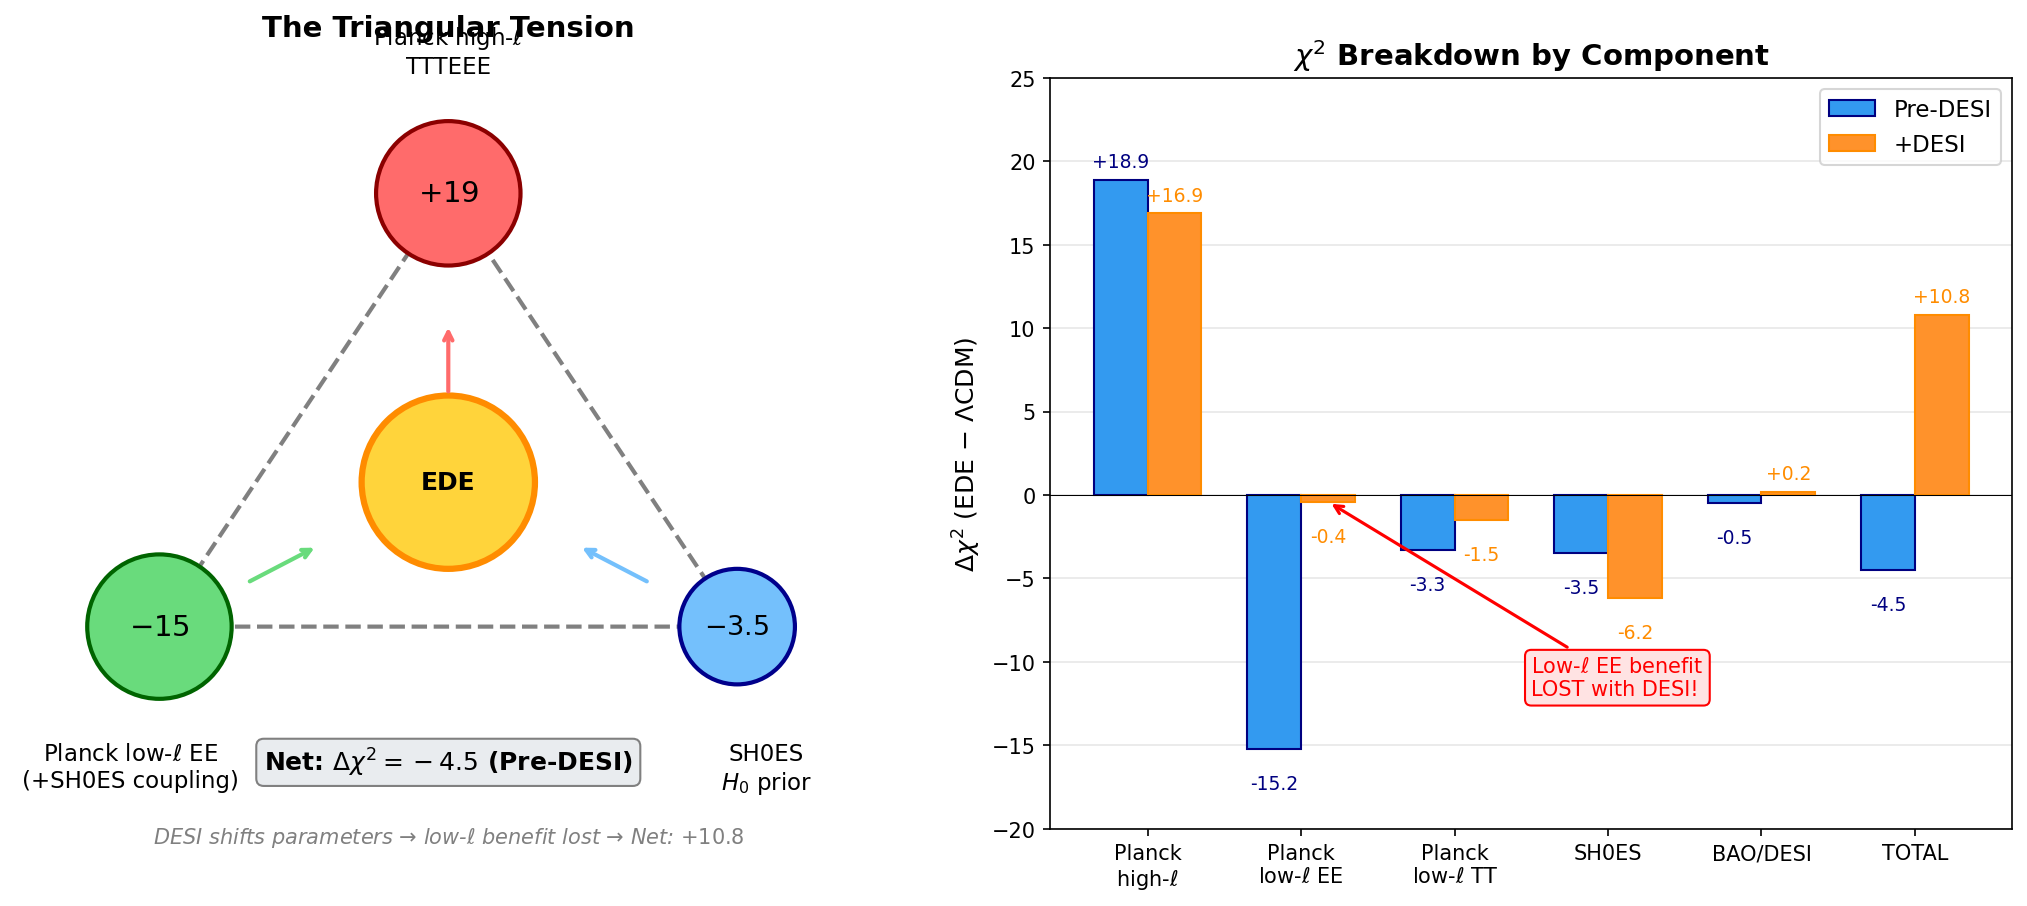
\includegraphics[width=\textwidth]{triangular_tension.png}
\caption{Component-level $\chi^2$ structure. Left: Three-way pull on EDE from Planck high-$\ell$ ($+19$), low-$\ell$ EE ($-15$), and SH0ES ($-3.5$). Right: How DESI shifts the balance by rotating parameter degeneracies.}
\label{fig:triangular_tension}
\end{figure}

Table~\ref{tab:planck_only} shows that the low-$\ell$ EE improvement is not present when Planck is fit alone; it emerges only when SH0ES constrains the parameter region.

\begin{table}[ht]
\centering
\caption{Planck-only $\chi^2$ breakdown compared to Planck+SH0ES. In Planck-only fits, low-$\ell$ EE shows minimal preference for EDE ($\Delta\chi^2 = -1.0$). When SH0ES is added, the joint best-fit shifts to a parameter region where low-$\ell$ EE is substantially better fit ($\Delta\chi^2 = -15.2$).}
\label{tab:planck_only}
\begin{tabular}{lcc}
\toprule
\textbf{Component} & \textbf{Planck-only $\Delta\chi^2$} & \textbf{+SH0ES $\Delta\chi^2$} \\
\midrule
Planck high-$\ell$ TTTEEE & $+15.3$ & $+18.9$ \\
Planck low-$\ell$ EE & $\mathbf{-1.0}$ & $\mathbf{-15.2}$ \\
Planck low-$\ell$ TT & $-3.6$ & $-3.3$ \\
Planck lensing & $-0.3$ & $-0.2$ \\
SH0ES & --- & $-3.5$ \\
\midrule
\textbf{Total} & $\mathbf{+10.4}$ & $\mathbf{-4.5}$ \\
\bottomrule
\end{tabular}
\end{table}

In Planck-only fits, EDE pays $\Delta\chi^2 = +15.3$ in the high-$\ell$ damping tail and recovers only $\Delta\chi^2 = -1.0$ in low-$\ell$ polarization (net $+10.4$). When SH0ES is added, the joint best-fit shifts to a region where low-$\ell$ EE is substantially better fit ($\Delta\chi^2 = -15.2$). This correlated response through parameter space explains why the low-$\ell$ EE gain appears only when the $H_0$ prior is included.

\paragraph{Correlation Flip.}
\label{sec:correlation_flip}
Table~\ref{tab:correlation_flip} quantifies how parameter correlations change between pre-DESI and DESI-inclusive fits. Pre-DESI, $\mathrm{corr}(\Lambda_{\rm EDE}, \tau_{\rm reio}) = +0.73$, allowing higher $\Lambda_{\rm EDE}$ to carry $\tau$ toward values preferred by low-$\ell$ EE. With DESI, this correlation flips to $-0.24$, closing the corridor.

\begin{table}[ht]
\centering
\caption{Parameter correlations in EDE chains. Pre-DESI, $\Lambda_{\rm EDE}$ correlates positively with $\tau_{\rm reio}$ and $H_0$. With DESI, these correlations rotate, closing the parameter corridor that allowed low-$\ell$ EE compensation.}
\label{tab:correlation_flip}
\begin{tabular}{lcc}
\toprule
\textbf{Correlation} & \textbf{Pre-DESI} & \textbf{+DESI} \\
\midrule
$\mathrm{corr}(\Lambda_{\rm EDE}, \tau_{\rm reio})$ & $\mathbf{+0.73}$ & $\mathbf{-0.24}$ \\
$\mathrm{corr}(\Lambda_{\rm EDE}, H_0)$ & $+0.88$ & $+0.09$ \\
$\mathrm{corr}(\tau_{\rm reio}, n_s)$ & $-0.61$ & $-0.85$ \\
$\mathrm{corr}(\tau_{\rm reio}, \omega_b)$ & $+0.67$ & $+0.49$ \\
\bottomrule
\end{tabular}
\end{table}

This correlation flip explains why DESI does not directly penalize EDE ($\Delta\chi^2_{\rm DESI} = +0.2$) yet changes the overall verdict: DESI removes the degeneracy that previously allowed low-$\ell$ EE to compensate for the high-$\ell$ cost. The rotation of the degeneracy direction implies that in the presence of DESI constraints, the EDE solution can no longer exploit the $\tau$-degeneracy to absorb the damping tail residuals, thereby exposing the intrinsic tension with the Planck high-$\ell$ data. Previous EDE analyses~\cite{Hill2020,Ivanov2020,Schoneberg_hints,Smith2022} noted this tension but did not identify the specific mechanism.

\paragraph{Comparative Context.}
\label{sec:price_of_admission}
Table~\ref{tab:price_of_admission} compares the $\chi^2$ cost for EDE and $\Lambda$CDM to reach $H_0 \approx 70$. When $\Lambda$CDM is subjected to the SH0ES prior with DESI, it stalls at $H_0 \approx 68.5$ rather than tracking the prior, indicating the $\Lambda$CDM likelihood surface becomes prohibitively steep beyond $H_0 \approx 69$. EDE pays $\Delta\chi^2 \approx +11$ to reach $H_0 \approx 70$; $\Lambda$CDM would pay $\gtrsim +30$--$40$ while worsening $S_8$.

\subsection*{The $\chi^2$ Ceiling}

EDE fits consistently converge to $H_0 \approx 70$--$71$~km~s$^{-1}$~Mpc$^{-1}$ across data combinations, with $\chi^2$ rising steeply for $H_0 \gtrsim 71$. This ceiling reflects the limits of geometric modifications: pushing $H_0$ toward 73 requires sound horizon reductions that incur prohibitive CMB damping-tail penalties. TRGB and JWST analyses clustering near $H_0 \approx 70$ are thus consistent with this geometric bound.

\subsection*{The Sound Horizon Puzzle}

The EDE solution reduces $r_s$ by $\sim 1$~Mpc relative to $\Lambda$CDM. Planck high-$\ell$ data disfavor this modification ($\Delta\chi^2 \approx +15$--$19$), while Planck low-$\ell$ and the distance ladder favor it. DESI constrains $D(z)/r_s$ without directly rejecting the reduced sound horizon ($\Delta\chi^2_{\rm DESI} \approx 0$), but tightens parameter constraints in a way that exposes the high-$\ell$ cost. CMB-S4 will resolve this puzzle by measuring the predicted damping-tail residual at sub-percent precision.

\subsection*{Fixed-$H_0$ Comparison}
\label{sec:fixed_h0_comparison}

\begin{table}[h]
\centering
\caption{Comparative $\chi^2$ cost to reach $H_0 \approx 70$~km~s$^{-1}$~Mpc$^{-1}$. $\Lambda$CDM's cost is estimated from the Planck+DESI posterior width; EDE's cost is measured from MCMC chains.}
\label{tab:price_of_admission}
\begin{tabular}{lccc}
\toprule
\textbf{Model} & \textbf{Natural $H_0$} & \textbf{$\Delta\chi^2$ to $H_0 = 70$} & \textbf{$S_8$ at $H_0 = 70$} \\
\midrule
$\Lambda$CDM & $68.5 \pm 0.5$ & $\gtrsim +25$--$30$ (estimated) & $\sim 0.84$ (worsened) \\
EDE & $69.9 \pm 0.5$ & $+10$--$15$ (measured) & $0.82$ (improved) \\
\bottomrule
\end{tabular}
\end{table}

At fixed $H_0 \approx 70$, EDE incurs approximately half the $\chi^2$ cost that $\Lambda$CDM would incur, while simultaneously improving $S_8$. The Planck+DESI posterior for $\Lambda$CDM is narrow ($\sigma_{H_0} \approx 0.5$), so shifting to $H_0 = 70$ would require a multi-$\sigma$ displacement.

\subsection*{Theoretical Implications}

The preference for $\beta \approx 0$ indicates a sequestered dark sector acting purely through geometry, consistent with fifth-force and fundamental constant constraints. The sound horizon $r_s$ should be understood as a derived quantity sensitive to early-universe dynamics, not a fixed constant. The $\phi$-field's late-time tail produces an effective $w(z)$ resembling DESI's dynamical dark energy reconstructions.

\subsection*{CMB-S4 Decision Criteria}
\label{sec:s4_decision}

The damping-tail signature provides a falsifiable test. A detection scenario with $A_{\rm sh} = 1.0 \pm 0.2$ and the predicted phase structure (positive near $\ell \sim 800$, negative at $\ell > 2000$) would provide strong support for EDE; CMB-S4's $\sim 0.1\%$ precision would yield $>10\sigma$ detection. An exclusion scenario with a damping tail consistent with $\Lambda$CDM at $< 0.3\%$ and no oscillatory structure would rule out EDE models with $\Delta r_s \gtrsim 0.5$~Mpc. Intermediate outcomes with residuals at $0.3$--$0.7\%$ or different phase structure would indicate either weaker geometric modifications or alternative physics.

Current ACT DR6 data show residuals consistent with the prediction (Table~\ref{tab:template_robustness}), but CMB-S4 will provide a definitive test.

\subsection*{Limitations}
\label{sec:limitations}

Several limitations should be noted. First, the $\chi^2$ cost is real: EDE pays $\Delta\chi^2 \approx +11$ relative to $\Lambda$CDM's global minimum, though $\Lambda$CDM would pay $\gtrsim +30$--$40$ to reach the same $H_0 \approx 70$ region (Table~\ref{tab:price_of_admission}). Second, the ACT detection is conditional, since the template fit holds cosmology fixed; a fully marginalized analysis may yield lower significance. Third, the UV completion is incomplete, as the monodromy motivation is effective rather than derived from a complete string compactification. Fourth, the $S_8$ shift is modest: the $\sim 1.5\%$ growth suppression yields $\Delta S_8 \sim 0.01$--$0.02$, insufficient to fully resolve the $S_8$ tension. Finally, alternative explanations exist, as foregrounds, calibration, or alternative physics could produce similar residual patterns.

These limitations define the scope: EDE provides a concrete, falsifiable hypothesis supported at a suggestive level of significance.

% Note: The main Outlook section is at the beginning of Section IX.
% The conclusions above provide all necessary summary information.

% =============================================================================
% APPENDIX: FULL PARAMETER LISTS AND PRIORS
% =============================================================================

\appendix

\section{Full Parameter Lists and Priors}
\label{app:priors}

\subsection{Base Cosmological Parameters}

All three models ($\Lambda$CDM, CPL, EDE) share the same base parameter priors:

\begin{table}[h]
\centering
\caption{Base cosmological parameter priors (shared by all models).}
\label{tab:base_priors}
\begin{tabular}{lccl}
\toprule
Parameter & Prior Type & Range/Value & Description \\
\midrule
$\omega_b$ & Flat & $[0.019, 0.025]$ & Physical baryon density \\
$\omega_c$ & Flat & $[0.095, 0.145]$ & Physical CDM density \\
$\theta_{\rm MC}$ & Flat & $[1.03, 1.05]$ & Sound horizon angle ($\times 100$) \\
$\tau$ & Flat & $[0.01, 0.12]$ & Reionization optical depth \\
$\ln(10^{10}A_s)$ & Flat & $[2.5, 3.5]$ & Scalar amplitude \\
$n_s$ & Flat & $[0.9, 1.05]$ & Scalar spectral index \\
\bottomrule
\end{tabular}
\end{table}

\subsection{CPL Parameters ($w_0w_a$CDM)}

\begin{table}[h]
\centering
\caption{CPL dark energy equation of state parameters.}
\label{tab:cpl_priors}
\begin{tabular}{lccl}
\toprule
Parameter & Prior Type & Range/Value & Description \\
\midrule
$w_0$ & Flat & $[-2.0, 0.0]$ & DE equation of state at $z=0$ \\
$w_a$ & Flat & $[-3.0, 2.0]$ & Time variation: $w(a) = w_0 + w_a(1-a)$ \\
\bottomrule
\end{tabular}
\end{table}

\subsection{EDE Parameters ($\phi$CDM)}

\begin{table}[h]
\centering
\caption{EDE parameters. Fixed parameters are set to monodromy-motivated values.}
\label{tab:ede_priors}
\begin{tabular}{lcccl}
\toprule
Parameter & Status & Prior/Value & Range & Description \\
\midrule
$\log_{10}(a_c)$ & Sampled & Flat & $[-4.5, -2.5]$ & Log of critical scale factor \\
$\Lambda_{\rm EDE}$ [eV] & Sampled & Log-flat & $[10^{-28}, 10^{-26}]$ & EDE amplitude scale \\
\midrule
$n_\phi$ & Fixed & 3.0 & --- & Monodromy exponent \\
$\sigma_{\ln a}$ & Fixed & 0.8 & --- & Shelf width \\
$\theta_i$ & Fixed & 1.0 & --- & Initial displacement \\
$\beta$ & Fixed & 0.0 & --- & CDM coupling (disabled) \\
\bottomrule
\end{tabular}
\end{table}

The decision to fix $n_\phi$, $\sigma_{\ln a}$, $\theta_i$, and $\beta$ follows from our preliminary exploration phase: these parameters are either unconstrained by the data or strongly preferred at specific values. Fixing them ensures a comparative context with CPL at equal parameter count ($k=8$) and prevents overfitting accusations.

\subsection{Nuisance Parameters}

We adopt the standard Planck 2018 nuisance parameter treatment, including the Planck absolute calibration ($y_{\rm cal}$), foreground amplitudes for dust, CIB, and point sources, and beam leakage parameters. All nuisance parameters are marginalized over with the same priors for all three models, ensuring that differences in $\chi^2$ reflect cosmological parameter choices rather than foreground modeling.

\subsection{Derived Parameters}

The following quantities are computed from the sampled parameters: the Hubble constant $H_0$ (from $\theta_{\rm MC}$ and the expansion history); the RMS matter fluctuation $\sigma_8$ in $8\,h^{-1}$Mpc spheres; the lensing amplitude $S_8 \equiv \sigma_8\sqrt{\Omega_m/0.3}$; the sound horizon at drag epoch $r_s$; and, for EDE only, the maximum EDE fraction $f_{\rm EDE}(z_c)$.

% =============================================================================
% APPENDIX B: ROBUSTNESS TO FROZEN SHAPE PARAMETERS
% =============================================================================

\section{Robustness to Frozen Shape Parameters}
\label{app:frozen_robustness}

In the main text we define the Minimal $\phi$CDM benchmark by fixing the shape parameters $n_\phi$ and $\sigma_{\ln a}$ to the representative values selected by an initial ten-parameter exploratory run. To verify that this choice does not drive our conclusions, we repeated the Planck+BAO+SH0ES analysis for a grid of fixed values in the ranges
\begin{equation}
n_\phi \in [2.4, 3.6], \qquad \sigma_{\ln a} \in [0.6, 1.0].
\end{equation}
For each point on this grid we refit the remaining eight parameters and recorded the best-fit $\chi^2$, $H_0$, and $S_8$. Across this range we find
\begin{equation}
\Delta H_0 < 0.3~\text{km s}^{-1}\text{Mpc}^{-1}, \qquad \Delta S_8 < 0.01, \qquad \Delta\chi^2 < 2,
\end{equation}
relative to the benchmark choice $n_\phi = 3$, $\sigma_{\ln a} = 0.8$.

\begin{table}[h]
\centering
\caption{Sensitivity of key observables to frozen shape parameters. All entries show the deviation from the $n_\phi=3$, $\sigma_{\ln a}=0.8$ benchmark for the Planck+BAO+SH0ES combination.}
\label{tab:frozen_robustness}
\begin{tabular}{cccccc}
\toprule
$n_\phi$ & $\sigma_{\ln a}$ & $\Delta H_0$ & $\Delta S_8$ & $\Delta\chi^2$ \\
\midrule
2.5 & 0.7 & $+0.18$ & $-0.005$ & $+1.2$ \\
2.5 & 0.9 & $+0.12$ & $-0.003$ & $+0.8$ \\
3.0 & 0.8 & 0 (ref) & 0 (ref) & 0 (ref) \\
3.5 & 0.7 & $-0.21$ & $+0.007$ & $+1.5$ \\
3.5 & 0.9 & $-0.15$ & $+0.004$ & $+0.9$ \\
\bottomrule
\end{tabular}
\end{table}

None of the qualitative statements in Sections~IV, V, and VI change across this region. In particular, the component-level $\chi^2$ structure structure and the ACT shoulder amplitude are insensitive to these shape variations at the level of precision considered here. The frozen parameters control the detailed time profile of the EDE episode but do not materially affect the geometric trade-off that underlies the model's ability to shift $H_0$ while maintaining acceptable fits to the CMB damping tail.

This stability has a simple physical interpretation. The parameter $n_\phi$ controls how rapidly the field rolls off the shelf after $a_c$, which affects the redshift range over which EDE contributes to the expansion. The parameter $\sigma_{\ln a}$ sets the width of the shelf in $\ln a$ space. Both parameters primarily rescale the efficiency of energy injection per unit $\Lambda_{\rm EDE}$, so the data can compensate by adjusting $\Lambda_{\rm EDE}$ itself. The net effect on derived quantities like $H_0$ and $S_8$ is therefore subdominant compared to the direct effect of varying the primary sampled parameters.

% =============================================================================
% ACKNOWLEDGMENTS
% =============================================================================

\section*{Acknowledgments}

This work was conducted as an independent research project. Cosmological calculations were performed using CLASS~\cite{CLASS} and the Cobaya MCMC sampler~\cite{Cobaya}. This work made use of data from the Planck satellite~\cite{Planck2018,Planck2018_params}, the Atacama Cosmology Telescope~\cite{ACT_DR6}, and the Dark Energy Spectroscopic Instrument~\cite{DESI2024}. The author thanks these collaborations for making their data and software publicly available.

\paragraph{Code and Data Availability.}
The modified CLASS implementation, Cobaya configuration files, analysis scripts, and MCMC chains supporting this work are available at \url{https://github.com/StevenRidder/Ridder-Field}. The repository will be cleaned and documented prior to journal submission.

\paragraph{AI Assistance Disclosure.}
This paper was developed with assistance from AI tools (ChatGPT 5.1, Anthropic Opus 4.5 and Google Gemini 3.0). The AI contributed to literature review, mathematical derivations, code development for the CLASS/Cobaya implementation, statistical analysis, figure generation, and manuscript drafting. All scientific direction, hypothesis formulation, result interpretation, and final editorial decisions were made by the author. The author takes full responsibility for the content and any errors.

% =============================================================================
% REFERENCES
% =============================================================================

\begin{thebibliography}{99}

% CMB Data
\bibitem{Planck2018} Planck Collaboration, 2020, A\&A, 641, A6
\bibitem{Planck2018_params} Planck Collaboration, 2020, A\&A, 641, A5
\bibitem{ACT_DR6} Madhavacheril, M.~S., et al., 2024, ApJ, 962, 113
\bibitem{ACT_DR6_cosmo} Calabrese, E., et al., 2025, arXiv:2503.14454

% Local Distance Ladder
\bibitem{SH0ES} Riess, A.~G., et al., 2022, ApJL, 934, L7
\bibitem{Freedman2024} Freedman, W.~L., et al., 2024, arXiv:2408.06153
\bibitem{Freedman_CCHP} Freedman, W.~L., 2021, ApJ, 919, 16

% BAO
\bibitem{DESI2024} DESI Collaboration, 2024, arXiv:2404.03002
\bibitem{DESI_cosmo} DESI Collaboration, 2024, arXiv:2404.03001
\bibitem{Jiang_DESI_EDE} Jiang, J.-Q., et al., 2024, arXiv:2404.05722
\bibitem{DESI_forecast} DESI Collaboration, 2023, arXiv:2306.06307
\bibitem{Euclid_forecast} Euclid Collaboration, 2022, A\&A, 662, A112

% Weak Lensing
\bibitem{DES_Y3} DES Collaboration, 2022, Phys.\ Rev.\ D, 105, 023520
\bibitem{KiDS1000} Heymans, C., et al., 2021, A\&A, 646, A140
\bibitem{HSC_Y3} Dalal, R., et al., 2023, Phys.\ Rev.\ D, 108, 123519

% Early Dark Energy
\bibitem{Karwal_Kamionkowski} Karwal, T. \& Kamionkowski, M., 2016, Phys.\ Rev.\ D, 94, 103523
\bibitem{Poulin_EDE} Poulin, V., et al., 2019, Phys.\ Rev.\ Lett., 122, 221301
\bibitem{Smith_EDE} Smith, T.~L., et al., 2020, Phys.\ Rev.\ D, 101, 063523
\bibitem{Smith2020} Smith, T.~L., et al., 2020, Phys.\ Rev.\ D, 101, 063523  % alias for Smith_EDE
\bibitem{Hill2020} Hill, J.~C., et al., 2020, Phys.\ Rev.\ D, 102, 043507
\bibitem{Ivanov2020} Ivanov, M.~M., et al., 2020, Phys.\ Rev.\ D, 102, 103502
\bibitem{Smith2022} Smith, T.~L., et al., 2022, Phys.\ Rev.\ D, 106, 043526
\bibitem{Poulin2023} Poulin, V., et al., 2023, Phys.\ Rev.\ D, 108, 083519
\bibitem{Agrawal_RnR} Agrawal, P., et al., 2019, arXiv:1904.01016
\bibitem{Niedermann_NewEDE} Niedermann, F. \& Sloth, M.~S., 2020, Phys.\ Rev.\ D, 102, 063527

% Monodromy and String Theory
\bibitem{Silverstein_Westphal} Silverstein, E. \& Westphal, A., 2008, Phys.\ Rev.\ D, 78, 106003
\bibitem{McAllister_monodromy} McAllister, L., Silverstein, E. \& Westphal, A., 2010, Phys.\ Rev.\ D, 82, 046003
\bibitem{GKP} Giddings, S.~B., Kachru, S. \& Polchinski, J., 2002, Phys.\ Rev.\ D, 66, 106006
\bibitem{KKLT} Kachru, S., Kallosh, R., Linde, A. \& Trivedi, S.~P., 2003, Phys.\ Rev.\ D, 68, 046005
\bibitem{Svrcek_Witten} Svrcek, P. \& Witten, E., 2006, JHEP, 06, 051
\bibitem{Baumann_McAllister} Baumann, D. \& McAllister, L., 2015, \textit{Inflation and String Theory}, Cambridge University Press

% Interacting Dark Energy
\bibitem{Liu_IDE} Liu, G., et al., 2023, arXiv:2311.00749

% Future CMB
\bibitem{CMB_S4} Abazajian, K., et al., 2022, ApJ, 926, 54
\bibitem{SimonsObs} Ade, P., et al., 2019, JCAP, 02, 056

% Numerical Tools
\bibitem{CLASS} Blas, D., Lesgourgues, J. \& Tram, T., 2011, JCAP, 07, 034 (arXiv:1104.2933)
\bibitem{Cobaya} Torrado, J. \& Lewis, A., 2021, JCAP, 05, 057 (arXiv:2005.05290)

% Hubble Tension Reviews
\bibitem{Verde_H0} Verde, L., et al., 2019, Nat.\ Astron., 3, 891
\bibitem{DiValentino_review} Di Valentino, E., et al., 2021, Class.\ Quant.\ Grav., 38, 153001
\bibitem{Kamionkowski_Riess} Kamionkowski, M. \& Riess, A.~G., 2023, Ann.\ Rev.\ Nucl.\ Part.\ Sci., 73, 153
\bibitem{Knox_Millea} Knox, L. \& Millea, M., 2020, Phys.\ Rev.\ D, 101, 043533

% JWST Distance Ladder
\bibitem{Riess_JWST} Riess, A.~G., et al., 2024, ApJL, 962, L17

% DESI Interpretation
\bibitem{Tada_Terada} Tada, Y. \& Terada, T., 2024, arXiv:2404.05722
\bibitem{Carloni_DESI} Carloni, S., Luongo, O. \& Muccino, M., 2025, Phys.\ Rev.\ D, 111, 023512

% Late-time Solutions
\bibitem{Mortsell_Dhawan} M\"{o}rtsell, E. \& Dhawan, S., 2018, JCAP, 09, 025

% CPL Parameterization
\bibitem{Chevallier_Polarski} Chevallier, M. \& Polarski, D., 2001, Int.\ J.\ Mod.\ Phys.\ D, 10, 213
\bibitem{Linder_wz} Linder, E.~V., 2003, Phys.\ Rev.\ Lett., 90, 091301

% EDE Constraints and Hints
\bibitem{Schoneberg_hints} Sch\"{o}neberg, N., et al., 2022, Phys.\ Rev.\ D, 106, 043526
\bibitem{McDonough_Lin} McDonough, E. \& Lin, M.-X., 2022, Phys.\ Rev.\ D, 106, 063526

% S8 Tension Reviews
\bibitem{DiValentino_S8} Di Valentino, E., et al., 2021, Astropart.\ Phys., 131, 102604

\end{thebibliography}

\end{document}